% UCL Thesis LaTeX Template
%  (c) Ian Kirker, 2014
%
% A template/skeleton for PhD/MPhil/MRes theses.
%
% It uses a rather split-up file structure because this tends to
%  work well for large, complex documents.
% It is suggested to use one file per chapter, but you may wish to use more
%  or fewer separate files than that.
% Various bits of configuration have been separated into their
%  own files, to keep everything neat.
% Note that the \input command just streams in whatever file you give
%  it, while the \include command adds a page break, and does some
%  extra organisation to make compilation faster. Note that you cannot
%  use \include inside an \include-d file.
% It is suggested to use \input for settings and configuration files that
%  you always want to use, and \include for each section of content.
% If you do that, it also means you can use the \includeonly statement
%  to only compile up the section you are interested in.
% You might also want to put figures into their own files to be \input.


% Formatting and binding rules for theses are here:
%  https://www.ucl.ac.uk/students/exams-and-assessments/research-assessments/format-bind-and-submit-your-thesis-general-guidance

% This package goes first, because it checks all
%  your syntax for mistakes and some old-fashioned LaTeX commands.
% Note that you load your documentclass before
%  packages, because some packages change behaviour based on
%  your document settings.
% Also, for those confused by the RequirePackage here vs usepackage
%  elsewhere, usepackage cannot be used before the documentclass
%  command, while RequirePackage can. That is the only functional
%  difference.
\RequirePackage[l2tabu, orthodox]{nag}


% ------ Main document class specification ------
% The draft option here prevents the insertion of images,
%  and adds chunky black bars to boxes that are exceeding
%  the page width (to show that they are).
% The oneside option can optionally be replaced by twoside if
%  you intend to print double-sided. Note that this is
%  *specifically permitted* by the UCL thesis formatting
%  guidelines.
%
% Valid options are:
%  phd
%  mres
%  mphil
%\documentclass[12pt,phd,draft,a4paper,oneside]{ucl_thesis}
\documentclass[12pt,phd,a4paper,oneside]{ucl_thesis}


% Package configuration:
%  LaTeX uses "packages" to add extra commands and features.
%  Several useful ones exist, so they have been put in a
%   separate file.
% -------- Packages --------

% This package just gives you a quick way to dump in some sample text.
% You can remove it -- it's just here for the examples.
% \usepackage{blindtext}

% This package means empty pages (pages with no text) won't get stuff
%  like chapter names at the top of the page. It's mostly cosmetic.
\usepackage{emptypage}

% The graphicx package adds the \includegraphics command,
%  which is your basic command for adding a picture.
\usepackage{graphicx}

% The float package improves LaTeX's handling of floats,
%  and also adds the option to *force* LaTeX to put the float
%  HERE, with the [H] option to the float environment.
\usepackage{float}

% The amsmath package enhances the various ways of including
%  maths, including adding the align environment for aligned
%  equations.
\usepackage{amsmath}

% Use these two packages together -- they define symbols
%  for e.g. units that you can use in both text and math mode.
\usepackage{gensymb}
\usepackage{textcomp}
% You may also want the units package for making little
%  fractions for unit specifications.
%\usepackage{units}

% The setspace package lets you use 1.5-sized or double line spacing.
\usepackage{setspace}
\setstretch{1.5}

% That just does body text -- if you want to expand *everything*,
%  including footnotes and tables, use this instead:
%\renewcommand{\baselinestretch}{1.5}

% PGFPlots is either a really clunky or really good way to add graphs
%  into your document, depending on your point of view.
% There's waaaaay too much information on using this to cover here,
%  so, you might want to start here:
%   http://pgfplots.sourceforge.net/
%  or here:
%   http://pgfplots.sourceforge.net/pgfplots.pdf
\usepackage{pgfplots}
\pgfplotsset{compat=1.17} % <- this fixed axis labels in the version I was using

% PGFPlotsTable can help you make tables a little more easily than
%  usual in LaTeX.
% If you're going to have to paste data in a lot, I'd suggest using it.
%  You might want to start with the manual, here:
%  http://pgfplots.sourceforge.net/pgfplotstable.pdf
%\usepackage{pgfplotstable}

% These settings are also recommended for using with pgfplotstable.
%\pgfplotstableset{
%	% these columns/<colname>/.style={<options>} things define a style
%	% which applies to <colname> only.
%	empty cells with={--}, % replace empty cells with '--'
%	every head row/.style={before row=\toprule,after row=\midrule},
%	every last row/.style={after row=\bottomrule}
%}

% The mhchem package provides chemistry formula typesetting commands
%  e.g. \ce{H2O}
%\usepackage[version=3]{mhchem}

% And the chemfig package gives a weird command for adding Lewis
%  diagrams, for e.g. organic molecules
%\usepackage{chemfig}

% The linenumbers command from the lineno package adds line numbers
%  alongside your text that can be useful for discussing edits
%  in drafts.
% Remove or comment out the command for proper versions.
%\usepackage[modulo]{lineno}
% \linenumbers

% Alternatively, you can use the ifdraft package to let you add
%  commands that will only be used in draft versions
%\usepackage{ifdraft}

% For example, the following adds a watermark if the draft mode is on.
%\ifdraft{
%  \usepackage{draftwatermark}
%  \SetWatermarkText{\shortstack{\textsc{Draft Mode}\\ \strut \\ \strut \\ \strut}}
%  \SetWatermarkScale{0.5}
%  \SetWatermarkAngle{90}
%}

% The multirow package adds the option to make cells span
%  rows in tables.
\usepackage{multirow}

% Subfig allows you to create figures within figures, to, for example,
%  make a single figure with 4 individually labeled and referenceable
%  sub-figures.
% It's quite fiddly to use, so check the documentation.
\usepackage{subfig}

% The natbib package allows book-type citations commonly used in
%  longer works, and less commonly in science articles (IME).
% e.g. (Saucer et al., 1993) rather than [1]
% More details are here: http://merkel.zoneo.net/Latex/natbib.php
%\usepackage{natbib}

% The bibentry package (along with the \nobibliography* command)
%  allows putting full reference lines inline.
%  See:
%   http://tex.stackexchange.com/questions/2905/how-can-i-list-references-from-bibtex-file-in-line-with-commentary
% \usepackage{bibentry}

% The isorot package allows you to put things sideways
%  (or indeed, at any angle) on a page.
% This can be useful for wide graphs or other figures.
%\usepackage{isorot}

% The caption package adds more options for caption formatting.
% This set-up makes hanging labels, makes the caption text smaller
%  than the body text, and makes the label bold.
% Highly recommended.
\usepackage[format=hang,font=small,labelfont=bf]{caption}

% If you're getting into defining your own commands, you might want
%  to check out the etoolbox package -- it defines a few commands
%  that can make it easier to make commands robust.
\usepackage{etoolbox}

% The microtype package adds `micro-typographic extensions' which
% generally makes text more readable and hyphenation less likely.
\usepackage{microtype}

% SI units
\usepackage[
	group-digits=none,
	separate-uncertainty=true
]{siunitx}\sisetup{detect-all}

% mathematical intervals
\usepackage{interval}
\intervalconfig{soft open fences}

% Latin terms
\usepackage[abbreviations,british]{foreign}

% more maths commands
\usepackage{amssymb}

% physics commands
\usepackage{physics}

% table commands
\usepackage{booktabs}

% symbol fonts
\usepackage{pifont}

% latex drawings
\usepackage{tikz}

% overlay drawings
\usepackage{overpic}

% UTF-8
\usepackage[utf8]{inputenc}
\usepackage[T1]{fontenc}

% indenting second line in a paragraph
\usepackage[notquote]{hanging}

% customise gaps between list items
\usepackage[shortlabels]{enumitem}

% highlights
\usepackage{soul}


% Sets up links within your document, for contents page entries
%  and references, and also PDF metadata.
% Edit this!
%%
%% This file uses the hyperref package to make your thesis have metadata embedded in the PDF,
%%  and also adds links to be able to click on references and contents page entries to go to
%%  the pages.
%%

% Some hacks are necessary to make bibentry and hyperref play nicely.
% See: http://tex.stackexchange.com/questions/65348/clash-between-bibentry-and-hyperref-with-bibstyle-elsart-harv
% \usepackage{bibentry}
% \makeatletter\let\saved@bibitem\@bibitem\makeatother % chktex 21
\usepackage[luatex]{hyperref}
% \makeatletter\let\@bibitem\saved@bibitem\makeatother % chktex 21
\makeatletter
\AtBeginDocument{
	\hypersetup{
		pdfsubject={Signal Processing},
		pdfkeywords={Convolutions, Slepian Functions, 2-Sphere, Manifolds, Wavelets},
		pdfauthor={Patrick James Roddy},
		pdftitle={Slepian Wavelets for the Analysis of Incomplete Data on Manifolds},
	}
}
\makeatother

% smart figure referencing, needs to be called after hyperref
\usepackage[capitalise,compress,nameinlink]{cleveref}

% fix caption hyperlinks in figures
\usepackage{hypcap}

% don't reset footnote numbering
\counterwithout*{footnote}{chapter}

% refer to multiple footnotes
\crefformat{footnote}{#2\footnotemark[#1]#3}


% And then some settings in separate files.
% These settings are partly from:
%  http://mintaka.sdsu.edu/GF/bibliog/latex/floats.html

% They give LaTeX more options on where to put your figures, and may
%  mean that fewer of your figures end up at the tops of pages far
%  away from the thing they're related to.

% Alters some LaTeX defaults for better treatment of figures:
% See p.105 of "TeX Unbound" for suggested values.
% See pp. 199-200 of Lamport's "LaTeX" book for details.

%   General parameters, for ALL pages:
\renewcommand{\topfraction}{0.9}	% max fraction of floats at top
\renewcommand{\bottomfraction}{0.8}	% max fraction of floats at bottom

%   Parameters for TEXT pages (not float pages):
\setcounter{topnumber}{2}
\setcounter{bottomnumber}{2}
\setcounter{totalnumber}{4}     % 2 may work better
\setcounter{dbltopnumber}{2}    % for 2-column pages
\renewcommand{\dbltopfraction}{0.9}	% fit big float above 2-col. text
\renewcommand{\textfraction}{0.2}	% page must be at least 20% text,
%                                  less than that and we get a floatpage

%   Parameters for FLOAT pages (not text pages):
\renewcommand{\floatpagefraction}{0.7}	% require fuller float pages
% N.B.: floatpagefraction MUST be less than topfraction !!
\renewcommand{\dblfloatpagefraction}{0.7}	% require fuller float pages

% remember to use [htp] or [htpb] for placement,
% e.g.
%  \begin{figure}[htp]
%   ...
%  \end{figure}

% figure location
\graphicspath{{figures/}}
 % For things like figures and tables
\usepackage[
	backend=biber,
	backref=true,
	dashed=false,
	date=year,
	eprint=false,
	isbn=false,
	maxnames=100,
	sorting=none,
	style=ieee,
	url=false
]{biblatex}
\addbibresource{library.bib}
   % For bibliographies
% ---------------------------
%% renew commands first
% ---------------------------

% fixed size absolute
\renewcommand{\abs}[1]{\big\lvert#1\big\rvert}

% fixed size braket
\NewCommandCopy{\oldbraket}{\braket}
\renewcommand{\braket}[1]{\oldbraket*{#1}}

% divergence
\renewcommand{\div}{\text{div}}

% fixed size expectation
\NewCommandCopy{\oldexpval}{\expval}
\renewcommand{\expval}[1]{\oldexpval*{#1}}

% gradient
\renewcommand{\grad}[1]{\nabla#1}

% fixed size 2-norm
\renewcommand{\norm}[1]{{\big\lVert#1\big\rVert}_{2}}

% bold matrices should be italic
\NewCommandCopy{\oldvb}{\vb}
\renewcommand{\vb}[1]{\oldvb*{#1}}

% ---------------------------
%% then new commands
% ---------------------------

% nice tilde
\newcommand{\almost}[1]{{\thicksim}#1}

% axisymmetric spherical harmonic indices
\newcommand{\axiHarmonic}[2][]{{#2}_{\ell#1 0}}

% conjugate
\newcommand{\conj}[1]{#1^{\ast}}

% sifting convolution of two functions
\newcommand{\convolution}[2]{(#1 \circledcirc{} #2)}

% diagonal matrix
\newcommand{\diag}[1]{\text{diag}\{#1\}} % chktex 21

% Slepian matrix
\newcommand{\Dmatrix}{D_{\ell{} m,\ell' m'}}

% edges
\newcommand{\edges}{\mathcal{E}}

% spherical harmonic factor
\newcommand{\factor}[1][]{\frac{2\ell#1+1}{4\pi}}

% FWHM
\newcommand{\fwhm}[1]{\text{FWHM}=\SI{#1}{\degree}}

% graph
\newcommand{\graph}{\mathcal{G}}

% spherical harmonic indices
\newcommand{\harmonic}[2][]{{#2}_{\ell#1 m#1}}

% spherical harmonic sum
\newcommand{\harmonicSum}[1][]{\sum\limits_{\ell#1 m#1}}

% Hermitian conjugate
\newcommand{\hermitian}[1]{#1^{\dagger}}

% Hilbert space
\newcommand{\hilbert}[1]{L^{2}(#1)} % chktex 36

% max harmonic mesh index
\newcommand{\imax}{i_{\text{max}}}

% integrate over the manifold
\newcommand{\integrateManifold}[1]{\int\limits_{\mathcal{M}} \dd{#1}}

% integrate over the region
\newcommand{\integrateRegion}[1]{\int\limits_{R} #1}

% intergral over SO3
\newcommand{\integrateRotation}[1]{\int\limits_{\text{SO(3)}} \dd{\rho(#1)}} % chktex 36

% integral over S2
\newcommand{\integrateSphere}[1]{\int\limits_{\mathbb{S}^{2}} \dd{\Omega(#1)}}

% inverse spherical harmonic factor
\newcommand{\inverseFactor}[1][]{\frac{4\pi}{2\ell#1+1}}

% Laplace operator
\newcommand{\laplace}[1]{\Delta_{\mathcal{#1}}}

% manifold
\newcommand{\manifold}{\mathcal{M}}

% pixel space on mesh
\newcommand{\mesh}[1]{#1(x)}
\newcommand{\meshY}[1]{#1(y)}

% summing in harmonic space of the mesh
\newcommand{\meshSum}[1][]{\sum\limits_{i#1}}

% volume element of the mesh
\newcommand{\meshVolume}{\dd{x}}

% real space
\newcommand{\pixel}[2][]{#2(\omega#1)}

% real positive parameter
\newcommand{\realPosParam}{\mathbb{R}_{\ast}^{+}}

% rotated function
\newcommand{\rotation}[1]{\mathcal{R}_{#1}}

% SO3
\newcommand{\rotationGroup}{\text{SO(3)}} % chktex 36

% set of inputs
\newcommand{\set}[1]{\{#1\}} % chktex 21

% Slepian coefficients
\newcommand{\slepian}[2][]{{#2}_{p#1}}

% Slepian sum
\newcommand{\slepianSum}[1][]{\sum\limits_{p#1}}

% signal-to-noise
\newcommand{\snr}[1]{\text{SNR}(#1)} % chktex 36

% sphere volume element
\newcommand{\sphereVolume}{\dd{\Omega(\omega)}}

% translated function
\newcommand{\translation}[1]{\mathcal{T}_{#1}}

% S2
\newcommand{\twoSphere}{\mathbb{S}^{2}}

% variance
\newcommand{\variance}[1]{{\big[\Delta#1\big]}^{2}}

% vertices
\newcommand{\vertices}{\mathcal{V}}

% Wigner D matrices
\newcommand{\wigner}[4][]{D^{#2#1}_{#3#4}}

% sum over wavelet coefficients
\newcommand{\waveletSum}{\sum\limits_{j=J_{0}}^{J}}
         % For maths

% These control how many number sections your subsections will take
%    such as Section 2.3.1.5.6.3
%  and how many of those will get put into the contents pages.
\setcounter{secnumdepth}{3}
\setcounter{tocdepth}{3}

% catch overfull box
\overfullrule=2cm

\begin{document}

% \nobibliography*
% ^-- A trick that works with the bibentry package to let
%  you put bibliography entries wherever you like.
% Use this to put references to papers a chapter's work was
%  published in at the end of that chapter.
% For more information, see: http://stefaanlippens.net/bibentry

% If you have not finished making your full BibTex file yet, you
%  might find this useful -- it will just replace all your
%  citations with little superscript notes.
% Uncomment to use.
%\renewcommand{\cite}[1]{\emph{\textsuperscript{[#1]}}}

% At last, content! Remember filenames are case-sensitive and
%  *must not* include spaces.
% This may change in a future version,
%  but given that some people needed it, if you need a different degree title
%  (e.g. Master of Science, Master in Science, Master of Arts)
%  uncomment the following 3 lines and set as appropriate (this *has* to be before \maketitle)
% \makeatletter
% \renewcommand {\@degree@string} {Master of Things}
% \makeatother

\title{Slepian Wavelets for the Analysis of Incomplete Data on Manifolds}
\author{Patrick James Roddy}
\department{Centre for Doctoral Training in Data Intensive Science}

\maketitle
\makedeclaration{}

\begin{abstract} % 300 word limit
	Many fields in science and engineering measure data that inherently live on non-Euclidean geometries, such as the sphere.
	It is increasingly important that techniques developed in the Euclidean setting are extended to other geometries.
	Due to recent interest in geometric deep learning, analogues of Euclidean techniques must also handle general manifolds or graphs.
	Often, data are only observed over partial regions of manifolds, and thus standard whole manifold techniques may not yield accurate predictions.
	In this thesis, a new wavelet basis is designed for datasets like these.

	Although many definitions of spherical convolutions exist, none fully emulate the Euclidean definition.
	A novel spherical convolution is developed, designed to tackle the shortcomings of existing methods.
	The so-called sifting convolution exploits the sifting property of the Dirac delta and follows by the inner product of a function with the translated version of another.
	This translation operator is analogous to the Euclidean translation in harmonic space and exhibits some useful properties.
	In particular, the sifting convolution supports directional kernels; has an output that remains on the sphere; and is efficient to compute.
	The convolution is entirely generic and thus may be used with any set of basis functions.
	An application of the sifting convolution with a topographic map of the Earth demonstrates that it supports directional kernels to perform anisotropic filtering.

	Slepian wavelets are built upon the eigenfunctions of the Slepian concentration problem of the manifold --- a set of bandlimited functions which are maximally concentrated within a given region.
	Wavelets are constructed through a tiling of the Slepian harmonic line by leveraging the scale-discretised framework.
	A straightforward denoising formalism demonstrates a boost in signal-to-noise for both a spherical and manifold example.
	Whilst these wavelets were inspired by spherical datasets like in cosmology, the wavelet construction may be utilised for manifold or graph data.
\end{abstract}

\begin{impactstatement}

	UCL theses now have to include an impact statement. The following text is the description from the guide linked from the formatting and submission website of what that involves. (Link to the guide: {\scriptsize \url{http://www.grad.ucl.ac.uk/essinfo/docs/Impact-Statement-Guidance-Notes-for-Research-Students-and-Supervisors.pdf}})

	\begin{quote}
		The statement describes, in no more than 500 words, how the expertise, knowledge, analysis,
		discovery or insight presented in your thesis could be put to a beneficial use. Consider benefits both
		inside and outside academia and the ways in which these benefits could be brought about.

		The benefits inside academia could be to the discipline and future scholarship, research methods,
		the curriculum; they might be within your research area and within other
		research areas.

		The benefits outside academia could occur to commercial activity, social enterprise, professional
		practice, clinical use, public health, public policy design, public service delivery, laws, public
		discourse, culture, the quality of the environment or quality of life.

		The impact could occur locally, regionally, nationally or internationally, to individuals, communities or
		organisations and could be immediate or occur incrementally, in the context of a broader field of
		research, over many years, decades or longer.

		Impact could be brought about through disseminating outputs (either in scholarly journals or
		elsewhere such as specialist or mainstream media), education, public engagement, translational
		research, commercial and social enterprise activity, engaging with public policymakers and public
		service delivery practitioners, influencing ministers, collaborating with academics and non-academics.

		Further information including a searchable list of hundreds of examples of UCL impact outside of
		academia please see \url{https://www.ucl.ac.uk/impact/}. For thousands more examples, please see
		\url{http://results.ref.ac.uk/Results/SelectUoa}.
	\end{quote}
\end{impactstatement}

\begin{acknowledgements}
	Acknowledge all the things!
\end{acknowledgements}

\setcounter{tocdepth}{2}
% Setting this higher means you get contents entries for
%  more minor section headers.

\tableofcontents
\listoffigures
\listoftables

\chapter{Introduction}\label{sec:chapter1}

Many fields in science and engineering measure data which are intrinsically non-Euclidean in nature.
The sphere, in particular, features commonly in disciplines such as geophysics, planetary science, computer graphics, signal processing, and cosmology.
The latter of these serves as the primary motivation for the work performed in this thesis.
Of increasing importance is the necessity to translate methods developed in the Euclidean domain to other geometries, such as the sphere.
Inspired by recent interest in geometric deep learning, many methods may be generalised further to other manifolds besides the sphere.

Convolutions are a fundamental technique in signal processing.
The convolution is a mathematical operation between two signals which produces a third signal which expresses how the shape of one signal is affected by the other.
Upon selection of a suitable kernel, convolutions have enjoyed success in many applications, such as: smoothing, sharpening, high pass filtering, differentiation, and edge detection.
Initially developed in the one-dimensional Euclidean domain, convolutions have since been used extensively in the two-dimensional setting, primarily for images.
In the spherical domain, however, existing definitions often do not capture all aspects of the Euclidean definition.
Moreover, such a convolution would ideally be generalisable to other manifolds.

Another important technique in signal processing is projecting a signal onto an appropriate basis.
In Fourier analyses, a one-dimensional signal may be expressed as an infinite sum of sines and cosines.
A Fourier transform allows one to go from the representation of a signal in time into a representation in frequency.
The signal may then be analysed in more detail by performing a cut in frequency space and analysing the resulting components independently.
In the spherical setting, a signal on the surface of the sphere may be expressed as a weighted sum of the spherical harmonics.
Spherical harmonic transforms follow as an analogy of Fourier transforms, whereby one can transform between real space and harmonic space.
Wavelets may be used as an alternative basis, which have been extended to other geometries in recent times.
Wavelets enable one to analyse contributions of scale-dependent features in both space and scale.
Applications of wavelets include: computer vision, compression, denoising, and time series analysis.

Often data are only observed over a partial region of a particular manifold, \ie{} the sphere.
For example, strong foreground microwave emissions are typically removed in analyses of the cosmic microwave background which are caused by the Galactic bulge of the Milky Way.
Thus, whole sphere methods may not be suitable for accurate analysis.
By leveraging the Slepian concentration problem, one may find the set of bandlimited functions which are optimally concentrated within a particular region.
A signal restricted to a given region (due to a limited set of observations) may then be decomposed into this basis as before.
Initially developed in the one-dimensional Euclidean setting as a time-frequency concentration problem, the so-called Slepian functions have been used in spatial-spectral applications in geophysics, planetary sciences, and medical imaging.

\section{Outline}

The remainder of this thesis is organised as follows.

\begin{hangparas}{24pt}{1}
	\textbf{\cref{sec:chapter2}} reviews the mathematical foundations on which the work performed in the remainder of this thesis relies.

	\textbf{\cref{sec:chapter3}} presents a review of some spherical convolutions in the literature, before developing a new convolution which addresses the limitations of existing convolutions.
	The so-called sifting convolution supports directional kernels, has an output which remains on the sphere, and is efficient to compute.

	\textbf{\cref{sec:chapter4}} defines a novel spherical wavelet basis designed for incomplete spherical datasets.
	The so-called Slepian wavelets are built on the eigenfunctions of the Slepian spatial-spectral concentration problem on the sphere.
	A scale-discretised wavelet transform is introduced, which depends on the convolution introduced in \cref{sec:chapter3}.

	\textbf{\cref{sec:chapter5}} generalises the Slepian wavelets in \cref{sec:chapter4} to Riemannian manifolds.
	Translations and, thus, convolutions are typically not well-defined on manifolds.
	By leveraging the sifting convolution (\cf{} \cref{sec:chapter3}), convolutions may be performed in Fourier space with the eigenfunctions of the Laplace-Beltrami operator.

	\textbf{\cref{sec:chapter6}} sets out some concluding remarks, summarising the work performed in thesis and outlining potential areas of future research.
\end{hangparas}

\chapter{Sifting Convolution on the Sphere}\label{sec:chapter2}

This material is adapted from~\cite{Roddy2021}.

\section*{Abstract}

A novel spherical convolution is defined through the sifting property of the Dirac delta on the sphere.
The so-called sifting convolution is defined by the inner product of one function with a translated version of another, but with the adoption of an alternative translation operator on the sphere.
This translation operator follows by analogy with the Euclidean translation when viewed in harmonic space.
The sifting convolution satisfies a variety of desirable properties that are lacking in alternate definitions, namely: it supports directional kernels; it has an output which remains on the sphere; and is efficient to compute.
An illustration of the sifting convolution on a topographic map of the Earth demonstrates that it supports directional kernels to perform anisotropic filtering, while its output remains on the sphere.

\section{Introduction}

Many fields in science and engineering measure data on spherical manifolds, such as computer graphics~\cite{Ramamoorthi2004}, planetary science~\cite{Turcotte1981}, geophysics~\cite{Simons2006}, quantum chemistry~\cite{Choi1999}, cosmology~\cite{Bennett1996}, and computer vision~\cite{Cohen2018,Esteves2020,Cobb2021}.
Possible extensions to signal processing techniques developed in the Euclidean domain may be transferred to the spherical domain.
The convolution is an important signal processing technique between two signals defined on the 2-sphere, which is central to filtering --- an integral part of spherical analyses.

Many definitions of spherical convolutions exist in the literature.
A spherical convolution operator would ideally exhibit a variety of desirable properties --- such a spherical convolution would accept directional inputs (\ie{} functions that are \emph{not} invariant under azimuthal rotation), whilst having the output remain on the sphere.
Moreover, the convolution would be efficient to compute.
Existing convolutions such as the \emph{isotropic convolution} (\eg{}~\cite{McEwen2007,Wei2011,Kennedy2011}) and the \emph{left convolution}~\cite{Kennedy2011,Driscoll1994} restrict themselves to an axisymmetric kernel (\ie{} kernels that are invariant under azimuthal rotation).
The \emph{directional convolution} has an output which is not on the sphere (\eg{}~\cite{McEwen2007,Wandelt2001}).
Lastly, the \emph{commutative anisotropic convolution}~\cite{Sadeghi2012,Khalid2012} and the \emph{directional convolution} are computationally demanding.
No existing spherical convolution satisfies all three desirable properties.

This work presents an alternative spherical convolution, the \emph{sifting convolution}, defined through the sifting property of the Dirac delta --- in analogy to the Euclidean definition.
The convolution is anisotropic in nature and supports directional kernels.
The output remains on the sphere, even when both inputs are directional.
Moreover, the convolution is efficient to compute, and is commutative up to a complex conjugate.

The remainder of this chapter is as follows.
\cref{sec:chapter2_preliminaries} includes some mathematical preliminaries and reviews existing spherical convolutions in the literature.
\cref{sec:chapter2_sifting_convolution} introduces the proposed sifting convolution.
\cref{sec:chapter2_numerical_illustration} presents a demonstration of the convolution with a directional kernel.
Lastly, \cref{sec:chapter2_conclusion} sets out some concluding remarks.

\section{Mathematical Background and Problem Formulation}\label{sec:chapter2_preliminaries}

\subsection{Mathematical Preliminaries}

\subsubsection{Signals on the Sphere}

Consider a complex valued square-integrable function \(\pixel{f}\) on the 2-sphere
%
\begin{equation}
	\twoSphere{}
	%
	= \set{\omega \in \mathbb{R}^{3} : \norm{\omega} = 1}.
\end{equation}
%
Here \(\omega=(\theta,\phi)\) parameterise a point on the unit sphere, where \(\theta \in \interval{0}{\pi}\) is the colatitude and \(\phi \in \interval[open right]{0}{2\pi}\) is the longitude.
The functions \(\pixel{f}\) form the Hilbert space \(\hilbert{\twoSphere}\).
The complex inner product induces a norm
%
\begin{equation}
	\norm{f}
	%
	= \sqrt{\braket{f}}.
\end{equation}
%
Signals on the sphere are functions with a finite induced norm.

\subsubsection{Spherical Harmonics}

The spherical harmonics are the complete orthonormal set of basis functions of the Hilbert space \(\hilbert{\twoSphere}\).
By the completeness of spherical harmonics, any \(f \in \hilbert{\twoSphere}\) may be decomposed as
%
\begin{equation}
	\pixel{f}
	%
	= \sum\limits_{\ell=0}^{\infty} \sum\limits_{m=-\ell}^{\ell} \harmonic{f} \pixel{\harmonic{Y}},
\end{equation}
%
where \(\harmonic{f}\) are the spherical harmonic coefficients given by
%
\begin{equation}
	\harmonic{f}
	%
	= \integrateSphere{\omega} \pixel{f} \pixel{\conj{\harmonic{Y}}}.
\end{equation}
%
The phase convention adopted here is
%
\begin{equation}
	\conj{\harmonic{Y}}
	%
	= {(-1)}^{m} Y_{\ell(-m)}
\end{equation}
%
such that
%
\begin{equation}
	\conj{\harmonic{f}}
	%
	= {(-1)}^{m} f_{\ell(-m)}
\end{equation}
%
for a real field.
One often considers signals on the sphere with a bandlimit of \(L\), \ie{} signals such that \(\harmonic{f} = 0,\ \forall \ell \geq L\); and adopts the shorthand notation
%
\begin{equation}
	\harmonicSum
	%
	= \sum\limits_{\ell=0}^{L-1} \sum\limits_{m=-\ell}^{\ell}.
\end{equation}

\subsubsection{Dirac Delta}

The Dirac delta on the sphere satisfies the following normalisation and sifting properties, respectively:
%
\begin{equation}
	\integrateSphere{\omega} \pixel{\delta}
	%
	= 1
\end{equation}
%
and
%
\begin{equation}
	\integrateSphere{\omega} \pixel{\delta_{\omega'}} \pixel{\conj{f}}
	%
	= \pixel[']{f},
\end{equation}
%
where \(\pixel{\delta_{\omega'}}\) represents the Dirac delta rotated to some \(\omega'=(\theta',\phi')\).
The harmonic expansion of the Dirac delta is
%
\begin{equation}\label{eq:chapter2_dirac_omega}
	\pixel{\delta_{\omega'}}
	%
	= \harmonicSum \pixel[']{\conj{\harmonic{Y}}} \pixel{\harmonic{Y}},
\end{equation}
%
which follows trivially by the sifting property.

\subsubsection{Rotation of a Signal on the 2-Sphere}

The Euler angles may parameterise three-dimensional rotations with \(\rho = (\alpha,\beta,\gamma) \in \rotationGroup{}\), where \(\alpha \in \interval[open right]{0}{2\pi}\), \(\beta \in \interval{0}{\pi}\), and \(\gamma \in \interval[open right]{0}{2\pi}\).
The rotation operator \(\rotation{\rho}\) consists of the sequence of rotations:
%
\begin{inparaenum}[(i)]
	\item \({\gamma}\) rotation about the \(z\)-axis;
	\item \({\beta}\) rotation about the \(y\)-axis; and
	\item \({\alpha}\) rotation about the \(z\)-axis.
\end{inparaenum}
%
The rotation of a function on the sphere is defined by
%
\begin{equation}
	\pixel{(\rotation{\rho}f)}
	%
	= f(\vb{R}_{\rho}^{-1} \omega),
\end{equation}
%
where \(\vb{R}_{\rho}\) is the three-dimensional rotation matrix corresponding to \(\rotation{\rho}\).
The spherical harmonic coefficients of a rotated function read
%
\begin{equation}\label{eq:chapter2_rotation_matrix}
	\harmonic{(\rotation{\rho}f)}
	%
	= \sum\limits_{m'=-\ell}^{\ell} \wigner{\ell}{m'}{m}(\rho) f_{\ell m'},
\end{equation}
%
where \(\wigner{\ell}{m'}{m}(\rho)\) are \emph{Wigner D matrices} which form the \(2\ell+1\)-dimensional representation of the rotation group for a given \({\ell}\).

\subsection{Spherical Convolutions}\label{sec:chapter2_spherical_convolutions}

The conventional convolution between two functions on two-dimensional Euclidean space \(\mathbb{R}^{n}\) is
%
\begin{equation}
	(f \star g)(x)
	%
	= \int\limits_{\mathbb{R}^{2}} \dd{y} f(x-y) g(y),
\end{equation}
%
where \(x,\ y \in \mathbb{R}^{n}\).
The convolution is commutative
%
\begin{equation}
	f \star g
	%
	= g \star f.
\end{equation}
%
A spherical counterpart of the convolution is required for functions defined on the sphere.
Alternative definitions of such a convolution exist in the literature but, while already useful, lack certain desirable properties.

The properties desired in the spherical extension of the convolution include:
%
\begin{inparaenum}[(i)]
	\item the support of directional kernels;
	\item an output which remains on the sphere; and
	\item efficient computation.
\end{inparaenum}
%
A convolution is considered computationally efficient here if its computational cost is no greater than the cost of fast spherical harmonic transforms, \ie{} \(\mathcal{O}(L^{3})\) (\eg{}~\cite{Driscoll1994,McEwen2011}).
Formulations of spherical convolutions exist in the literature, but none satisfy all these properties.
A summary of existing spherical convolutions and their properties follows.

\subsubsection{Isotropic Convolution}

In real space the isotropic convolution (\eg{}~\cite{McEwen2007,Wei2011,Kennedy2011}) is
%
\begin{equation}
	\pixel{(f \odot g)}
	%
	= \integrateSphere{\omega'} \pixel[']{f} \pixel[']{\conj{(\rotation{\omega}g)}},
\end{equation}
%
which in harmonic space becomes (\eg{}~\cite{McEwen2007})
%
\begin{equation}\label{eq:chapter2_isotropic_harmonic}
	\harmonic{(f \odot g)}
	%
	= \sqrt{\inverseFactor} \harmonic{f} \conj{\axiHarmonic{g}},
\end{equation}
%
as
%
\begin{align}
	\pixel{(f \odot g)}
	%
	 & = \integrateSphere{\omega'} \pixel[']{f} \pixel[']{\conj{(\rotation{\omega}g)}} \nonumber{}                                                                                           \\
	%
	 & = \integrateSphere{\omega'} \harmonicSum \harmonic{f} \pixel[']{\harmonic{Y}} \harmonicSum['] \conj{\harmonic[']{(\rotation{\omega}g)}} \pixel[']{\conj{\harmonic[']{Y}}} \nonumber{} \\
	%
	 & = \harmonicSum \harmonic{f} \conj{\harmonic{(\rotation{\omega}g)}} \nonumber                                                                                                          \\
	%
	 & = \harmonicSum \harmonic{f} \conj{\big(\wigner{\ell}{m}{0}(\phi,\theta,0) \axiHarmonic{g}\big)} \nonumber{}                                                                           \\
	%
	 & = \harmonicSum \sqrt{\inverseFactor} \harmonic{f} \conj{\axiHarmonic{g}} \pixel{\harmonic{Y}},
\end{align}
%
where the last line follows through the relation
%
\begin{equation}
	\wigner[\ast]{\ell}{m}{0}(\phi,\theta,0)
	%
	= \sqrt{\inverseFactor} \pixel{\harmonic{Y}}.
\end{equation}
%
The isotropic convolution has the following properties:
%
\begin{inparaenum}[(i)]
	\item does not support directional kernels since \(\pixel{g}\) must be axisymmetric;
	\item an output which remains on the sphere; and
	\item efficient computation since it is a product in harmonic space.
\end{inparaenum}

\subsubsection{Left Convolution}

The definition of the left convolution~\cite{Kennedy2011,Driscoll1994} in real space is
%
\begin{equation}
	\pixel{(f \circleddash g)}
	%
	= \integrateRotation{\rho} f(\rho\eta) g(\rho^{-1}\omega),
\end{equation}
%
where \({\eta}\) is the north pole, and \(\dd{\rho(\rho)}=\sin{\beta} \dd{\alpha} \dd{\beta} \dd{\gamma}\) is the usual invariant measure on \(\rotationGroup{}\).
The harmonic representation of this convolution is
%
\begin{equation}
	\harmonic{(f \circleddash g)}
	%
	= 2\pi \sqrt{\inverseFactor} \harmonic{f} \axiHarmonic{g}.
\end{equation}
%
As the harmonic representations suggest, the isotropic and left convolutions are closely related, as elaborated in~\cite{Kennedy2011}.
Hence, the properties are similar.
The left convolution has the following properties:
%
\begin{inparaenum}[(i)]
	\item does not support directional kernels since \(\pixel{g}\) must be axisymmetric;
	\item an output which remains on the sphere; and
	\item efficient computation since it is a product in harmonic space.
\end{inparaenum}

\subsubsection{Directional Convolution}

Rotations on the sphere are the spherical counterpart of translations in the Euclidean domain in real space.
Hence, the standard directional convolution is
%
\begin{equation}\label{eq:chapter2_directional_convolution}
	(f \circledast g)(\rho)
	%
	= \integrateSphere{\omega} \pixel{f} \pixel{\conj{(\rotation{\rho}g)}}.
\end{equation}
%
Upon expanding in harmonic space, this becomes (\eg{}~\cite{McEwen2007,Wandelt2001})
%
\begin{equation}
	(f \circledast g) (\rho)
	%
	= \harmonicSum \harmonic{f} \sum\limits_{m'=-\ell}^{\ell} \conj{\big(\wigner{\ell}{m'}{m}(\rho) g_{\ell m'}\big)},
\end{equation}
%
as
%
\begin{align}
	(f \circledast g)(\rho)
	%
	 & = \integrateSphere{\omega} \pixel{f} \pixel{\conj{(\rotation{\rho}g)}} \nonumber{}                                                                                           \\
	%
	 & = \integrateSphere{\omega} \harmonicSum \harmonic{f} \pixel{\harmonic{Y}} \harmonicSum['] \conj{\harmonic[']{(\rotation{\rho}g)}} \pixel{\conj{\harmonic[']{Y}}} \nonumber{} \\
	%
	 & = \harmonicSum \harmonic{f} \conj{\harmonic[']{(\rotation{\rho}g)}} \nonumber{}                                                                                              \\
	%
	 & = \harmonicSum \harmonic{f} \sum\limits_{m'=-\ell}^{\ell} \conj{\big(\wigner{\ell}{m'}{m}(\rho) g_{\ell m'}\big)},
\end{align}
%
and hence, the output is on \(\rotationGroup{}\).
Fast algorithms exist~\cite{McEwen2007,Wandelt2001,Wiaux2007,McEwen2013}, but the convolution remains less efficient than a spherical harmonic transform.
The directional convolution has the following properties:
%
\begin{inparaenum}[(i)]
	\item does support directional kernels;
	\item an output which does not remain on the sphere due to the 3D rotation of the kernel; and
	\item expensive computation.
\end{inparaenum}

\subsubsection{Commutative Anisotropic Convolution}

The definition of the commutative anisotropic convolution~\cite{Sadeghi2012,Khalid2012} is
%
\begin{equation}
	\pixel{(f \oplus g)}
	%
	= \integrateSphere{\omega'} \pixel[']{(\rotation{(\phi,\theta,\pi-\phi)}f)} \pixel[']{g},
\end{equation}
%
which on expansion reads
%
\begin{equation}
	\pixel{(f \oplus g)}
	%
	= \harmonicSum \sum\limits_{m'=-\ell}^{\ell} \wigner{\ell}{m'}{m}(\phi,\theta,\pi-\phi) f_{\ell m'} \conj{\harmonic{g}}.
\end{equation}
%
The limitation here is that one must specify the initial rotation as \({\gamma=\pi-\alpha}\) in order for the convolution to be commutative.
The complexity of the convolution is \(\mathcal{O}(L^{3}\log{L})\), and hence, it is less efficient than a spherical harmonic transform.
The convolution has the following properties:
%
\begin{inparaenum}[(i)]
	\item it supports directional kernels;
	\item an output which remains on the sphere; and
	\item expensive computation.
\end{inparaenum}

\subsection{Problem Formulation}

\cref{tab:chapter2_properties} presents a summary of the spherical convolutions discussed and their properties.
No existing definition of a spherical convolution has all the desired properties discussed in \cref{sec:chapter2_spherical_convolutions}.
In this work, the sifting convolution, which satisfies all desirable properties, is presented.

\begin{table}
	\centering
	\caption{
		Properties of spherical convolutions.
	}\label{tab:chapter2_properties}
	\begin{tabular}{@{}rccc@{}}
		\toprule
		                        & Anisotropic & \(\twoSphere{}\) Output & Efficient \\
		\midrule
		Isotropic               & \ding{55}   & \ding{51}               & \ding{51} \\
		%
		Left                    & \ding{55}   & \ding{51}               & \ding{51} \\
		%
		Directional             & \ding{51}   & \ding{55}               & \ding{55} \\
		%
		Commutative Anisotropic & \ding{51}   & \ding{51}               & \ding{55} \\
		%
		Sifting (this work)     & \ding{51}   & \ding{51}               & \ding{51} \\
		\bottomrule
	\end{tabular}
\end{table}


\section{Sifting Convolution}\label{sec:chapter2_sifting_convolution}

This work defines the sifting convolution which permits directional kernels, whose output remains on the sphere and is efficient to compute.
Moreover, it is commutative up to a complex conjugate.
The sifting convolution is constructed using a novel translation operator defined on the sphere.

\subsection{Translation Operator}\label{sec:chapter2_translation_operator}

In real space, the rotation operator on the sphere is the usual analogue of the translation operator in the Euclidean setting.
One may define an alternative operator, \(\translation{\omega}\), which follows as the analogue of the Euclidean setting but in harmonic space.
This translation is in contrast to the standard rotation as it considers two angles rather than three and thereby its output remains on the sphere.
In practice the translation operator is defined as a product of basis functions.
In the Euclidean setting, \eg{} \(\mathbb{R}\), the complex exponentials
%
\begin{equation}
	\phi_{u}(x)
	%
	= \exp{iux},
\end{equation}
%
with \(x,\ u \in \mathbb{R}\) form the standard orthonormal basis.
A shift of coordinates defines the translation of the basis functions:
%
\begin{equation}
	\phi_{u}(x + x')
	%
	= \phi_{u}(x') \phi_{u}(x),
\end{equation}
%
with \(x' \in \mathbb{R}\) and where the final equality follows by the standard rule for exponents.
The definition of the translation of the spherical harmonics on the sphere follows by analogy with the representation as a product of basis functions:
%
\begin{equation}
	\pixel{(\translation{\omega'}\harmonic{Y})} \equiv \pixel[']{\harmonic{Y}} \pixel{\harmonic{Y}},
\end{equation}
%
where \(\omega'=(\theta',\phi')\).

This leads to a natural harmonic expression for the translation of a general arbitrary function \(f \in \hilbert{\twoSphere}\)
%
\begin{equation}\label{eq:chapter2_translation_real}
	\pixel{(\translation{\omega'}f)}
	%
	= \harmonicSum \harmonic{f} \pixel[']{\harmonic{Y}} \pixel{\harmonic{Y}},
\end{equation}
%
implying
%
\begin{equation}\label{eq:chapter2_translation_harmonic}
	\harmonic{(\translation{\omega'}f)}
	%
	= \harmonic{f} \pixel[']{\harmonic{Y}}.
\end{equation}
%
This translation operator is considered further in \cref{sec:chapter2_translation_interpretation} to build greater intuition.

\subsection{Convolution Operator}

With a translation operator to hand, one may define the sifting convolution on the sphere of \(f,\ g \in \hilbert{\twoSphere}\) in the usual manner by the inner product
%
\begin{equation}\label{eq:chapter2_convolution_real}
	\pixel{\convolution{f}{g}}
	%
	\equiv \braket{\translation{\omega}f}{g},
\end{equation}
%
noting the use of the alternative translation operator defined in \cref{sec:chapter2_translation_operator}.

In harmonic space this simplifies to the product
%
\begin{equation}\label{eq:chapter2_convolution_harmonic}
	\harmonic{\convolution{f}{g}}
	%
	= \harmonic{f} \conj{\harmonic{g}},
\end{equation}
%
as
%
\begin{align}
	\pixel{(f \circledcirc g)}
	%
	 & = \braket{\translation{\omega}f}{g} \nonumber{}                                                                                                                                         \\
	%
	 & = \integrateSphere{\omega'} \pixel[']{(\translation{\omega}f)} \pixel[']{\conj{g}} \nonumber{}                                                                                          \\
	%
	 & = \integrateSphere{\omega'} \harmonicSum \harmonic{f} \pixel[']{\harmonic{Y}} \pixel{\harmonic{Y}} \harmonicSum['] \conj{\harmonic[']{g}} \pixel[']{\conj{\harmonic[']{Y}}} \nonumber{} \\
	%
	 & = \harmonicSum \harmonic{f} \conj{\harmonic{g}} \pixel{\harmonic{Y}}.
\end{align}
%
Since the harmonic representation of the convolution is simply a product (again by analogy with the harmonic representation of the Euclidean convolution), it is efficient to compute.
Note that harmonic multiplication has been considered before~\cite{Kennedy2011}; although it has been used here to define a new anisotropic convolution operator, introducing a conjugation and elaborating a real space interpretation.

\subsection{Translation Interpretation}\label{sec:chapter2_translation_interpretation}

One may show that the translation operator is simply a (sifting) convolution of a function with the shifted Dirac delta function:
%
\begin{align}
	\pixel{\convolution{f}{\delta_{\omega'}}}
	%
	 & = \harmonicSum \harmonic{f} \pixel[']{\harmonic{Y}} \pixel{\harmonic{Y}} \nonumber{} \\
	%
	 & = \pixel{(\translation{\omega'}f)},
\end{align}
%
by noting \cref{eq:chapter2_convolution_harmonic} and where the final equality follows by \cref{eq:chapter2_translation_real}.
The sifting convolution and translation are thus natural analogues of the respective operators defined in Euclidean space.

\subsection{Properties}\label{sec:chapter2_properties}

The sifting convolution has all the desired properties discussed in \cref{sec:chapter2_spherical_convolutions}, namely, the convolution accepts directional inputs, has an output which remains on the sphere, and is efficient to compute.
\cref{tab:chapter2_properties} summarises the properties of the sifting convolution and compares them to the properties of alternative spherical convolutions.

The translation preserves symmetries, which means that any symmetry that exists in the initial kernel definition will be present after the translation.
Thus, one must be careful when choosing a kernel for a convolution to ensure it has the desired properties when translated, \eg{} spatial localisation.
To perform anisotropic smoothing that is localised (the usual interpretation), the translated kernel also needs to be localised.
If the kernel has, say, even azimuthal symmetry, when it is translated to \(\omega'=(\theta', \phi')\) it will have a localised component both at \(\phi'\) and \(-\phi'\).
While this is not a problem \emph{per se}, for the usual interpretation of smoothing one would desire a localised component at \(\phi'\) only.
This can be achieved by ensuring the original kernel does not exhibit a symmetry that would lead to multiple localised components once translated.
The \emph{harmonic Gaussian} introduced in \cref{sec:chapter2_numerical_illustration} satisfies the desired property.

\section{Numerical Illustration}\label{sec:chapter2_numerical_illustration}

This section demonstrates the effect of the sifting convolution through the application of a directional kernel to an example signal on the sphere.
Some potential kernels are defined in \cref{sec:chapter2_kernels}, where the effect of the translation is explored.
The convolution is then demonstrated with one of these kernels in \cref{sec:chapter2_convolution} on a topographic map of the Earth.
All later computations use the \texttt{SSHT}\footnote{\url{http://astro-informatics.github.io/ssht/}} code~\cite{McEwen2011}.

\subsection{Kernels}\label{sec:chapter2_kernels}

As discussed in \cref{sec:chapter2_properties}, the translation preserves symmetries from the initial kernel definition.
Hence, one must consider the desired properties in the translated kernel, \eg{} spatial localisation.

\subsubsection{Gaussian}

First, consider the standard axisymmetric Gaussian on the sphere, \ie{}
%
\begin{equation}
	\harmonic{\mathcal{G}}
	%
	= \exp(-\frac{{\ell}^{2}}{2\sigma^{2}}),
\end{equation}
%
where \(\sigma{}\) is the standard deviation of the Gaussian.
\cref{fig:chapter2_gaussian} presents the Gaussian kernel (left panel) and the result of the translation (right panel); where it is clear that the axisymmetric symmetry is preserved.
This function has no directional components and is therefore unsuitable for general convolution purposes.

\begin{figure}[htp]
	\centering\capstart{}
	\subfloat[\(\Re{\pixel{\mathcal{G}}}\)]{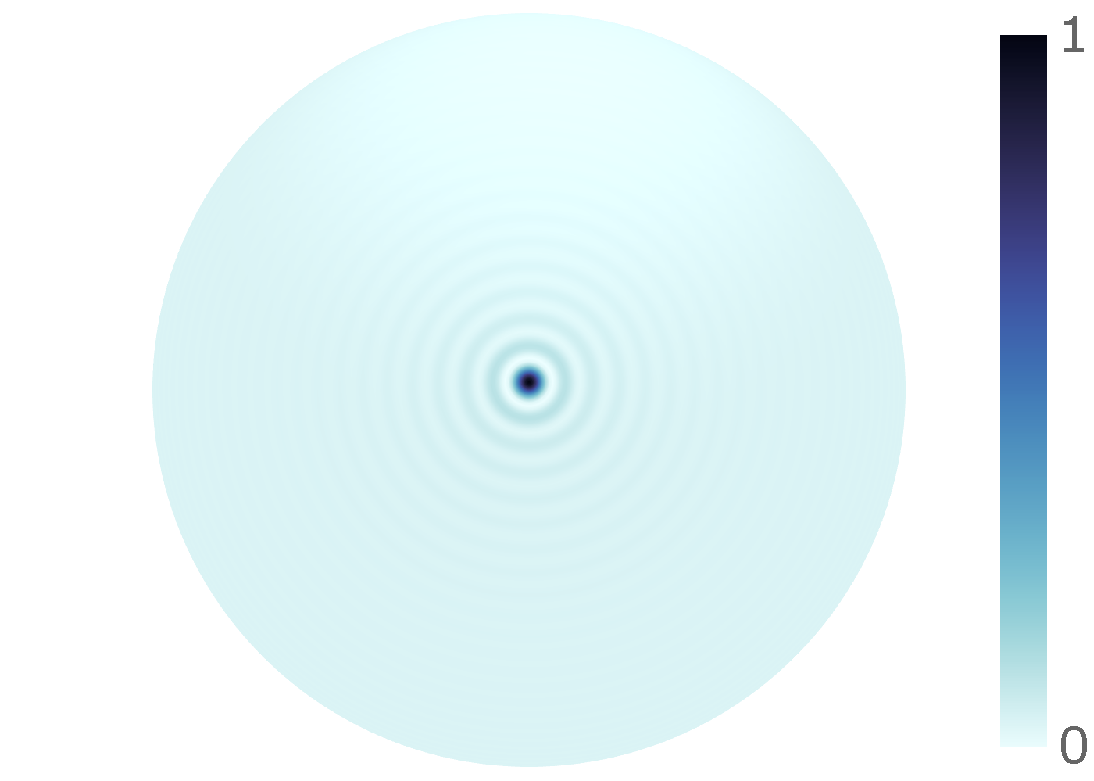
\includegraphics[trim={23 7 3 6},clip,width=.5\textwidth]{gaussian_1000sig_L128_res512_real_norm.pdf}}
	\hfill
	\subfloat[\(\Re{\pixel{(\translation{\omega'}\mathcal{G})}}\)]{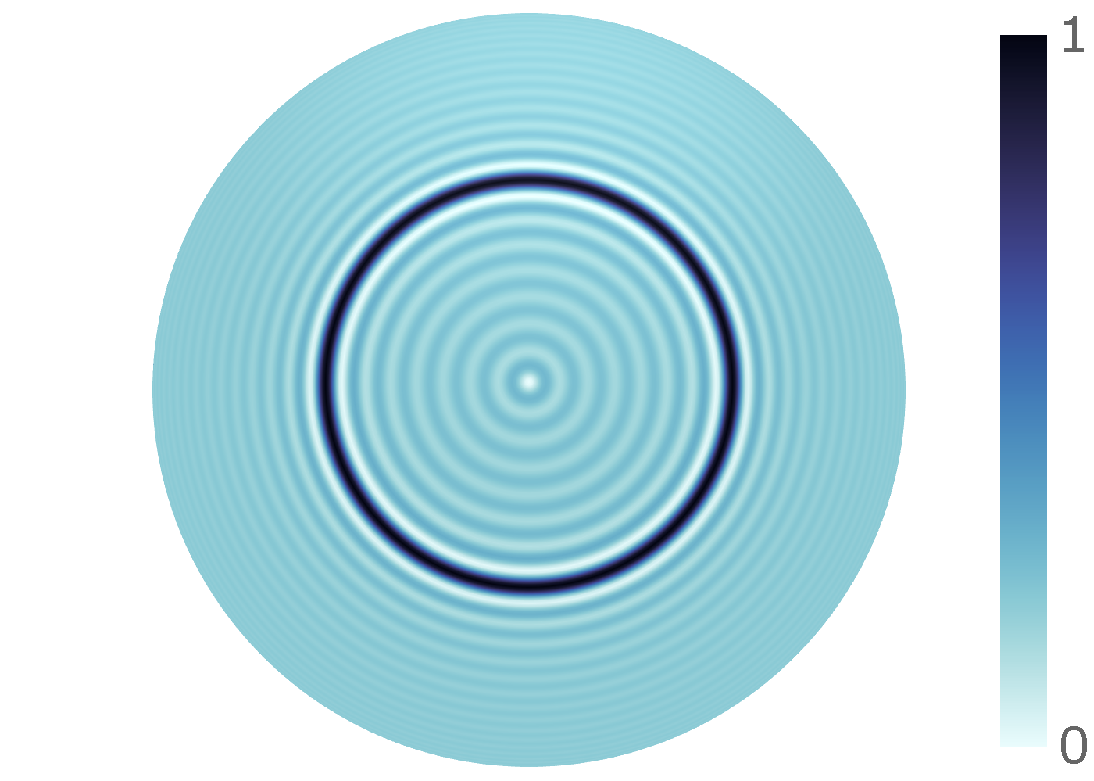
\includegraphics[trim={23 7 3 6},clip,width=.5\textwidth]{gaussian_1000sig_L128_translate_alpha3pi4_beta1pi8_res512_real_norm.pdf}}
	\caption[
		A Gaussian at the north pole and then translated
	]{
		Panel (a) presents the standard axisymmetric Gaussian (bandlimited at \(L=128\)).
		The Gaussian is then translated to some \(\omega'=(\theta',\phi')\), as shown in panel (b).
		Plainly, the axisymmetric symmetry has been preserved under translation.
		The colour is between zero and one, reflecting the scaled intensity of the field.
	}\label{fig:chapter2_gaussian}
\end{figure}


\subsubsection{Squashed Gaussian}

Define the \emph{squashed Gaussian} in real space as the standard Gaussian (\ie{} in the polar angle \(\theta{}\)) modulated by a sinusoidal function in the azimuthal angle \(\phi{}\) by
%
\begin{equation}
	\pixel{\mathcal{SG}}
	%
	= \mathcal{SG}(\theta,\phi)
	%
	= \exp\Bigg(-\frac{1}{2}{\bigg(\frac{\theta-\mean{\theta}}{\sigma_{\theta}}\bigg)}^{2}\Bigg)
	%
	\sin(\nu_{\phi}\phi),
\end{equation}
%
where \(\mean{\theta}\)/\(\sigma_{\theta}\) and \(\nu_{\phi}\) are parameters controlling the mean/standard deviation of the Gaussian and the frequency of the sine wave respectively.
The squashed Gaussian kernel is shown in the left panel of \cref{fig:chapter2_squashed_gaussian}, and the translated kernel is shown in the right panel.
The odd symmetry in the kernel definition results in the axisymmetric translated function.
Evidently, the squashed Gaussian is not suitable for smoothing purposes as the behaviour is similar to the axisymmetric Gaussian case.

\begin{figure}[htp]
	\centering
	\subfloat[\(\Re{\pixel{\mathcal{SG}}}\)]{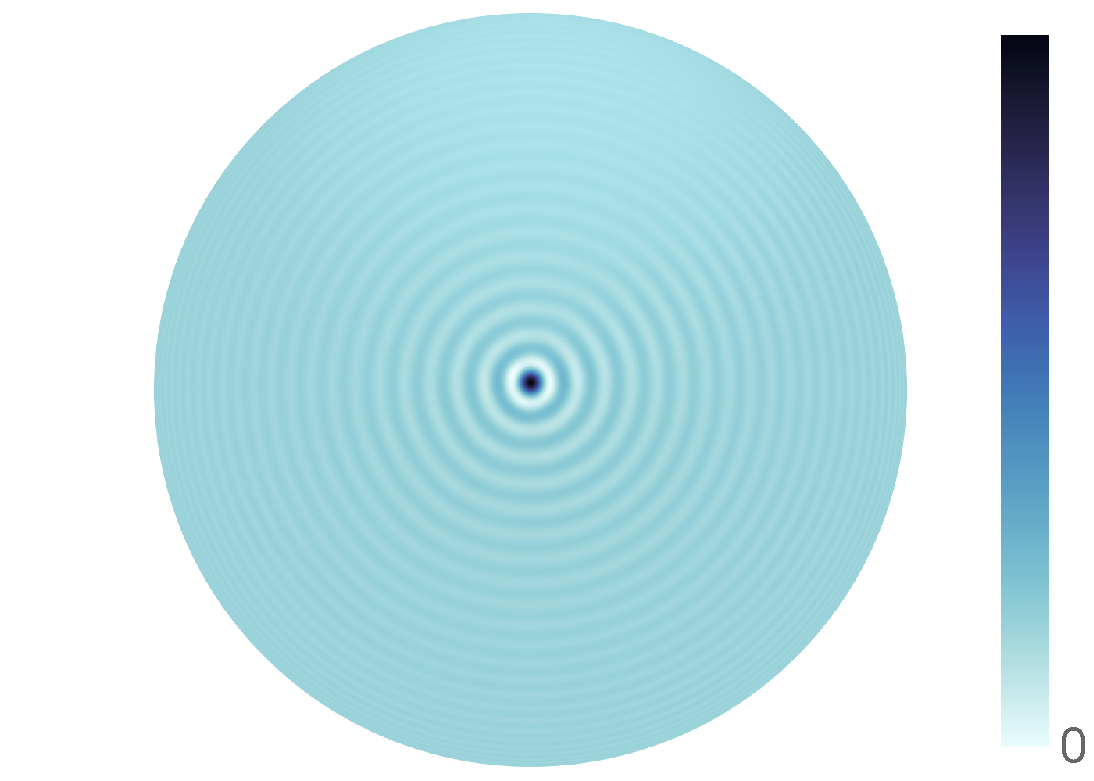
\includegraphics[trim={23 7 3 6},clip,width=.5\textwidth]{squashed_gaussian_1tsig100_1freq10_L128_res512_real_norm.pdf}}
	\hfill
	\subfloat[\(\Re{\pixel{(\translation{\omega'}\mathcal{SG})}}\)]{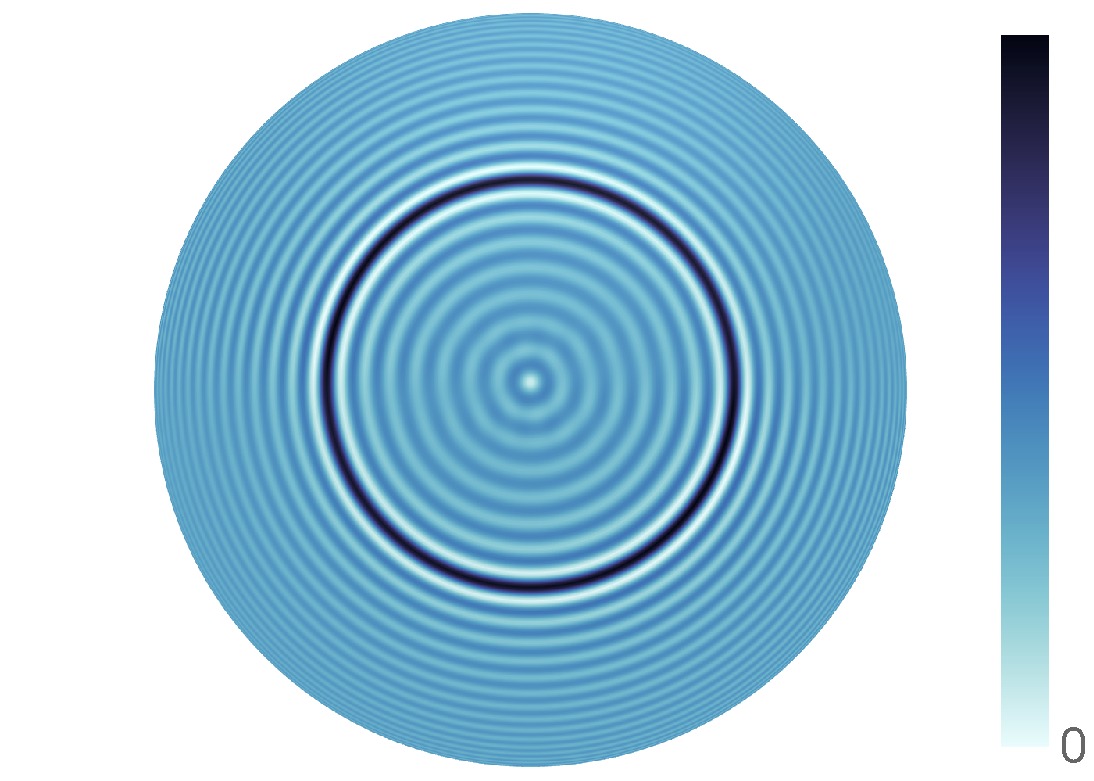
\includegraphics[trim={23 7 3 6},clip,width=.5\textwidth]{squashed_gaussian_1tsig100_1freq10_L128_translate_alpha3pi4_beta1pi8_res512_real_norm.pdf}}
	\caption{
		Panel (a) presents the squashed Gaussian (bandlimited at \(L=128\)).
		The squashed Gaussian is then translated to some \(\omega'=(\theta',\phi')\), as shown in panel (b).
		The odd azimuthal symmetry in the initial kernel definition is preserved under translation.
		The colour is between zero and one, reflecting the scaled intensity of the field.
	}\label{fig:chapter2_squashed_gaussian}
\end{figure}


\subsubsection{Elongated Gaussian}

Define the \emph{elongated Gaussian} as a two-dimensional Gaussian in real space in the polar angle \(\theta{}\) and the azimuthal angle \(\phi{}\) by
%
\begin{equation}
	\pixel{\mathcal{EG}}
	%
	= \mathcal{EG}(\theta,\phi)
	%
	= \exp\bigg(-\bigg(\frac{{(\theta-\mean{\theta})}^{2}}{2\sigma_{\theta}^{2}}
		%
		+ \frac{{(\phi-\mean{\phi})}^{2}}{2\sigma_{\phi}^{2}}\bigg)\bigg),
\end{equation}
%
where \((\mean{\theta},\mean{\phi})\) are the means, and \((\sigma_{\theta},\sigma_{\phi})\) are the standard deviations of the respective Gaussians.
The left panel of \cref{fig:chapter2_elongated_gaussian} presents the elongated Gaussian, and the right panel shows the result of the translation.
The elongated Gaussian has even azimuthal symmetry which results in two localised components at \(\phi'\) and \(-\phi'\) upon translation.
Thus, this kernel is not suitable for anisotropic smoothing.

\begin{figure}[htp]
	\centering\capstart{}
	\subfloat[\(\Re{\pixel{\mathcal{EG}}}\)]{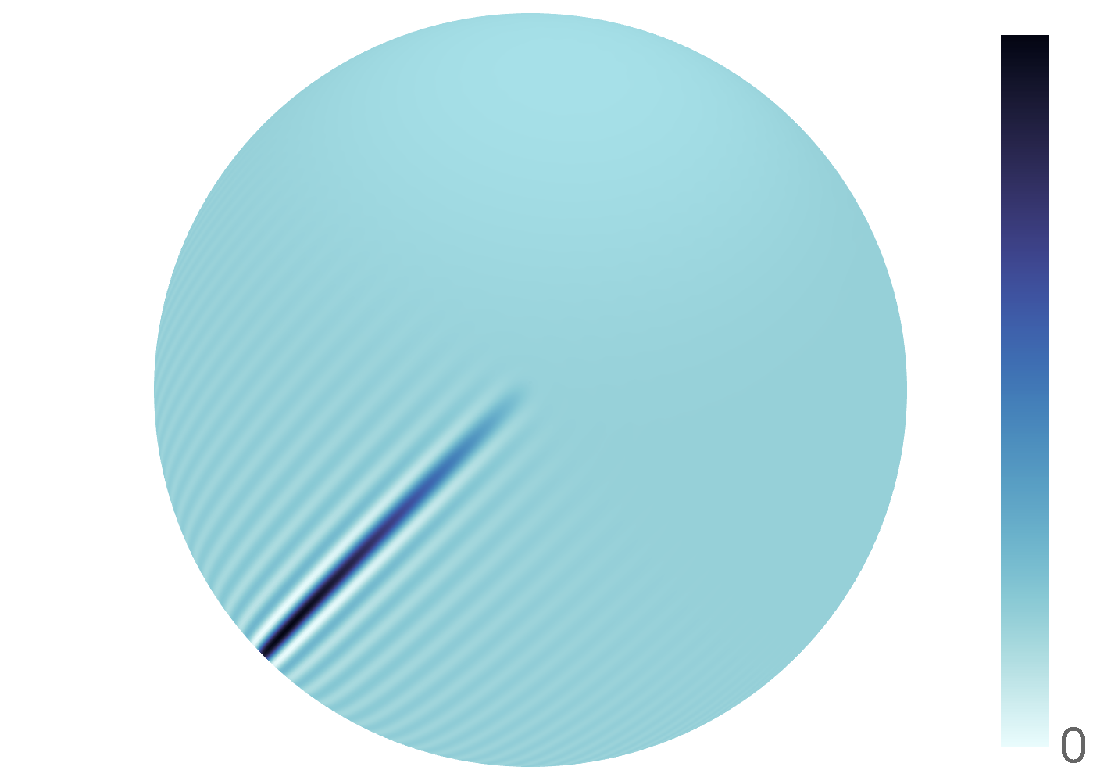
\includegraphics[trim={23 7 3 6},clip,width=.5\textwidth]{elongated_gaussian_1tsig_1psig1000_L128_res512_real_norm.pdf}}
	\hfill
	\subfloat[\(\Re{\pixel{(\translation{\omega'}\mathcal{EG})}}\)]{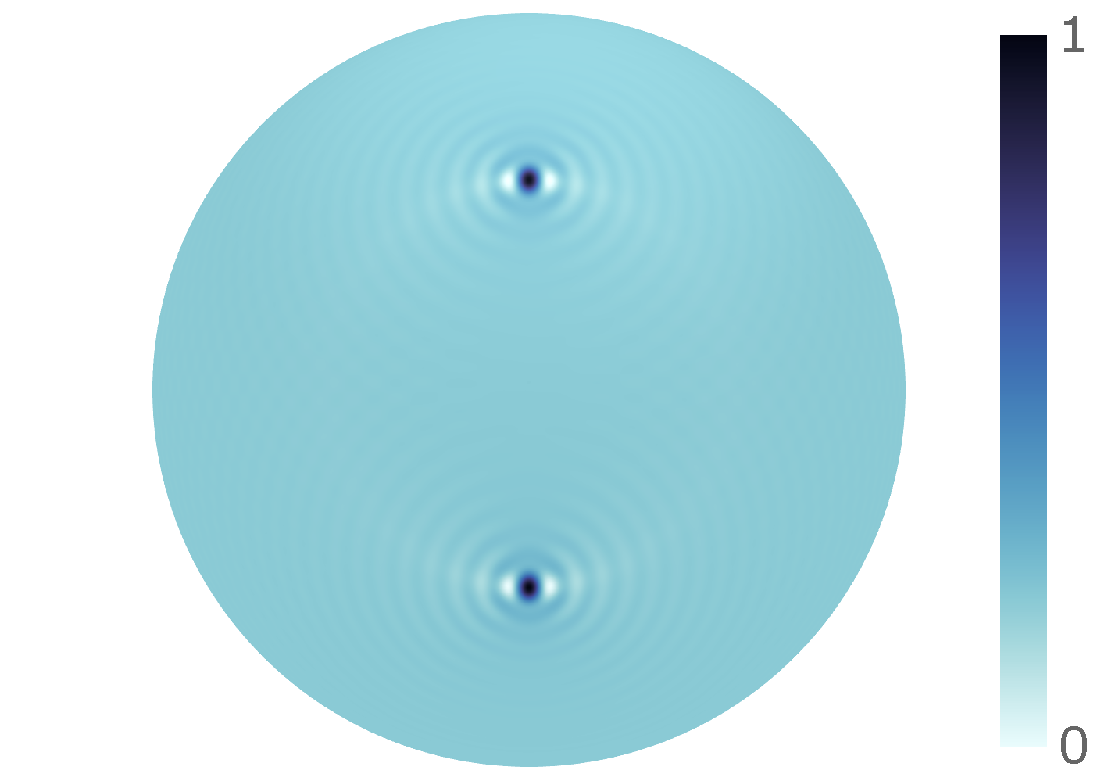
\includegraphics[trim={23 7 3 6},clip,width=.5\textwidth]{elongated_gaussian_1tsig_1psig1000_L128_translate_alpha3pi4_beta1pi8_res512_real_norm.pdf}}
	\caption[
		An elongated Gaussian at the north pole and then translated
	]{
		Panel (a) presents the elongated Gaussian (bandlimited at \(L=128\)) --- where the central bar in the plot extends over half of the sphere.
		The elongated Gaussian is then translated to some \(\omega'=(\theta',\phi')\), as shown in panel (b).
		The even azimuthal symmetry in the initial kernel definition results into the two localised components at \(\phi'\) and \(-\phi'\) under translation.
		The colour is between zero and one, reflecting the scaled intensity of the field.
	}\label{fig:chapter2_elongated_gaussian}
\end{figure}


\subsubsection{Harmonic Gaussian}

Define the \emph{harmonic Gaussian} as a two-dimensional Gaussian in harmonic space by
%
\begin{equation}\label{eq:chapter2_harmonic_gaussian}
	\harmonic{f}
	%
	= \exp(-\bigg(\frac{{\ell}^{2}}{2\sigma_{\ell}^{2}} + \frac{{m}^{2}}{2\sigma_{m}^{2}}\bigg)).
\end{equation}
%
In effect, this function is the standard axisymmetric Gaussian in \(\ell{}\) modulated by a Gaussian in \(m\).
Note this function is not real --- if required one can define only the positive \(m\) components and impose reality by the conjugate symmetry relationship in harmonic space.
The function is directional, and hence, is useful in illustrating the effect of the sifting convolution on the sphere.
Consider two differently sized harmonic Gaussians on the sphere to see the effect on the sifting convolution.
\cref{fig:chapter2_harmonic_gaussian} shows both an elongated (left panel) and symmetric (right panel) harmonic Gaussian (top panel) and the result of the translation (bottom panel).

\begin{figure}[htp]
	\centering
	\subfloat[\(\Re{f_{A}}\)]{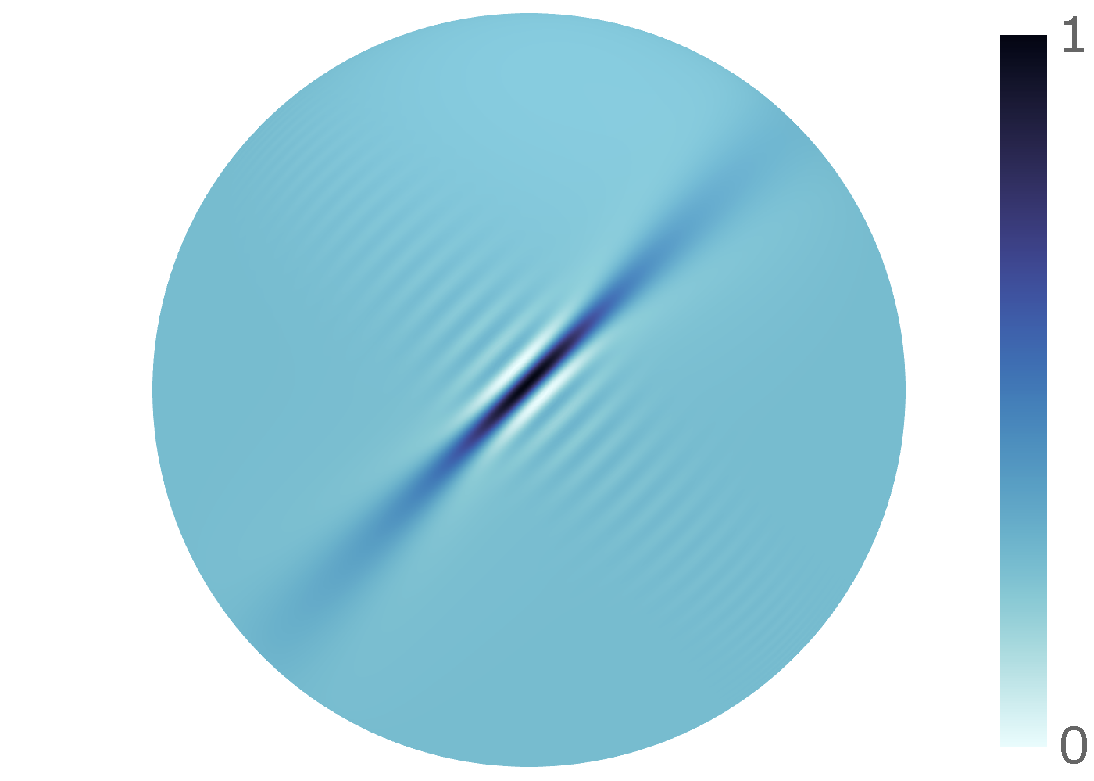
\includegraphics[trim={23 7 3 6},clip,width=.5\textwidth]{harmonic_gaussian_100lsig_10msig_L128_res512_real_norm.pdf}}
	\hfill
	\subfloat[\(\Re{f_{B}}\)]{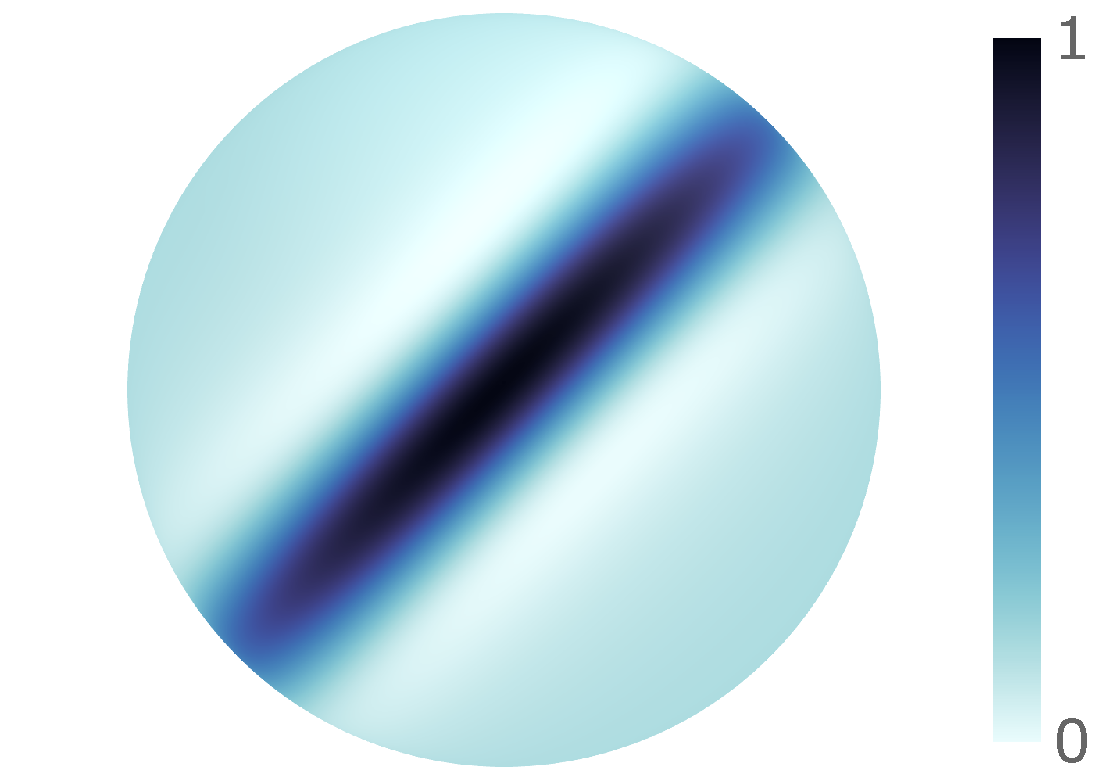
\includegraphics[trim={23 7 3 6},clip,width=.5\textwidth]{harmonic_gaussian_10lsig_10msig_L128_res512_real_norm.pdf}}
	\newline
	\subfloat[\(\Re{\pixel{(\translation{\omega'}f_{A})}}\)]{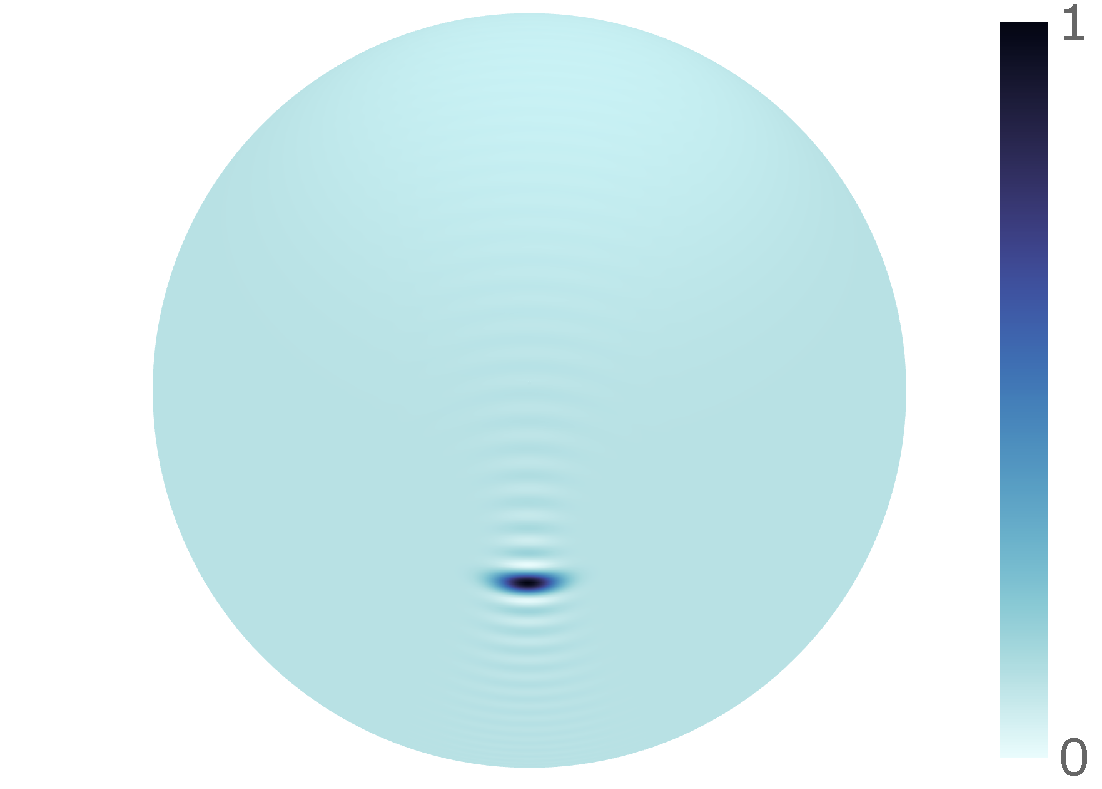
\includegraphics[trim={23 7 3 6},clip,width=.5\textwidth]{harmonic_gaussian_100lsig_10msig_L128_translate_alpha3pi4_beta1pi8_res512_real_norm.pdf}}
	\hfill
	\subfloat[\(\Re{\pixel{(\translation{\omega'}f_{B})}}\)]{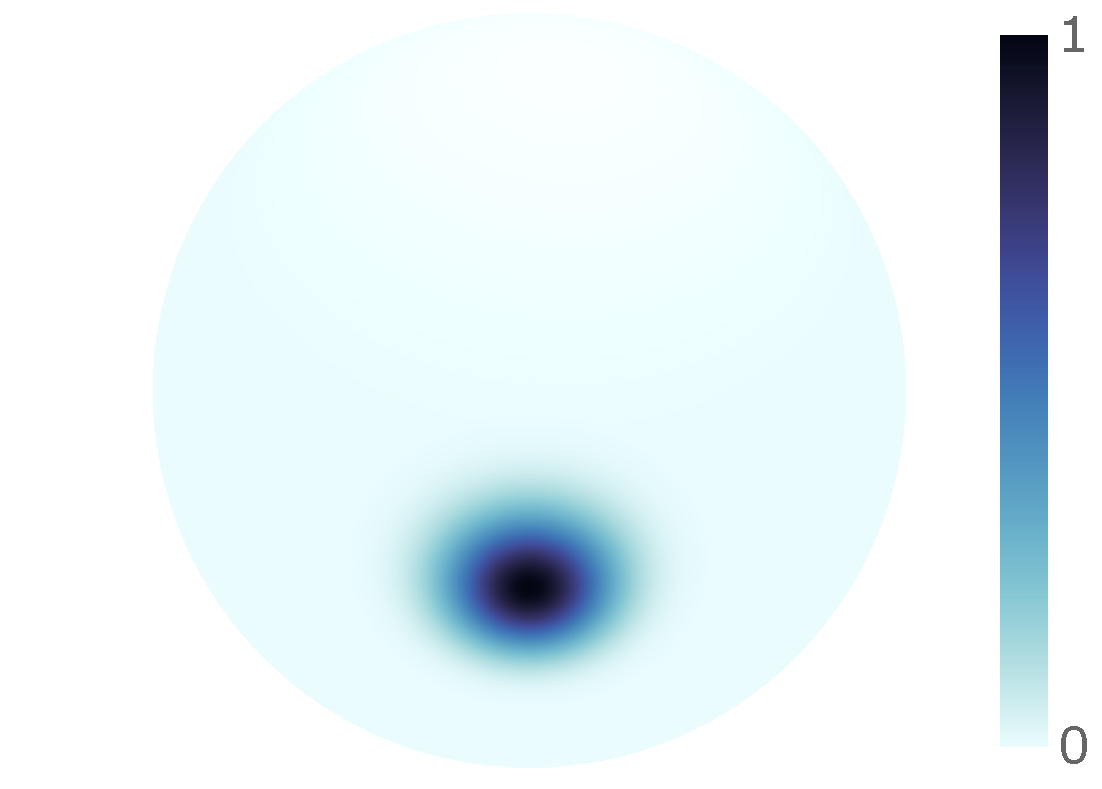
\includegraphics[trim={23 7 3 6},clip,width=.5\textwidth]{harmonic_gaussian_10lsig_10msig_L128_translate_alpha3pi4_beta1pi8_res512_real_norm.pdf}}
	\caption{
		The top row presents the harmonic Gaussian (bandlimited at \(L=128\)) for two different \((\sigma_{\ell},\sigma_{m})\) values (\cf{} \cref{eq:chapter2_harmonic_gaussian}).
		Panel (a) corresponds to a more elongated kernel \(f_{A}\), where \((\sigma_{\ell},\sigma_{m}) = (10^{2},10^{1})\).
		The harmonic Gaussian is translated to some \(\omega'=(\theta',\phi')\) as shown in panel (c).
		Whereas panel (b) corresponds to a more symmetric kernel \(f_{B}\), where \((\sigma_{\ell},\sigma_{m}) = (10^{1},10^{1})\), with the corresponding translated function in panel (d).
		The colour is between zero and one, reflecting the scaled intensity of the field.
	}\label{fig:chapter2_harmonic_gaussian}
\end{figure}


\subsection{Convolution}\label{sec:chapter2_convolution}

To study the effect of the sifting convolution, consider the \emph{Earth Gravitational Model EGM2008} dataset~\cite{Pavlis2013}.
This dataset is the topographic map of the Earth.
\cref{fig:chapter2_earth} presents the dataset up to an order of \(L=128\).
The sifting convolution is then performed between the Earth representation and the harmonic Gaussian with the resultant plot given in \cref{fig:chapter2_convolved}.
As expected, when the elongated kernel is considered, as shown in the left panel, the result exhibits greater anisotropic smoothing than when considering the symmetric kernel, as shown in the right panel.
It is clear that the sifting convolution supports directional kernels to perform anisotropic filtering (smoothing), while the output remains on the sphere.

\begin{figure}[htp]
	\centering
	\includegraphics[trim={22 9 7 6},clip,width=.5\textwidth]{chapter2/earth_L128_res512_real_norm.pdf}
	\caption{
		EGM2008 dataset centred on a view of South America (bandlimited at \(L=128\)).
		The colour is between zero and one, reflecting the scaled intensity of the field.
	}\label{fig:chapter2_earth}
\end{figure}


\begin{figure}[htpb]
	\centering\capstart{}
	\subfloat[\(\Re{\pixel{\convolution{f_{A}}{g}}}\)]{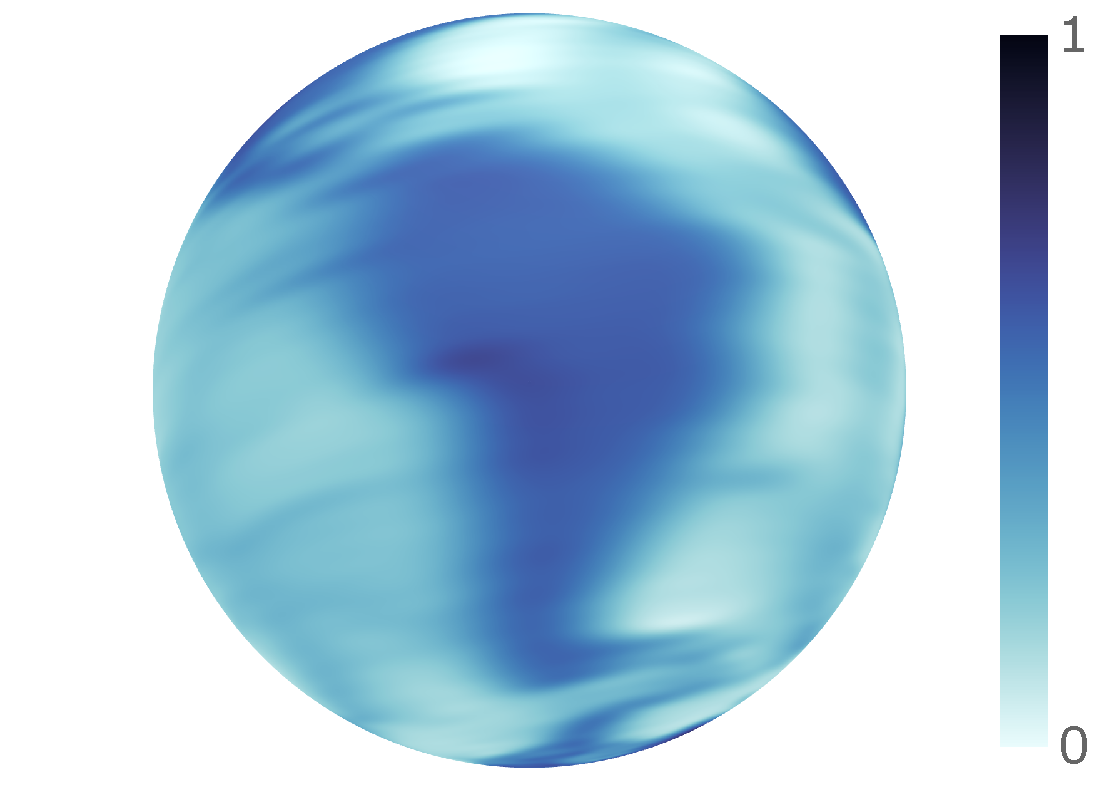
\includegraphics[trim={23 7 3 6},clip,width=.5\textwidth]{harmonic_gaussian_100lsig_10msig_L128_convolved_earth_L128_res512_real_norm.pdf}}
	\hfill
	\subfloat[\(\Re{\pixel{\convolution{f_{B}}{g}}}\)]{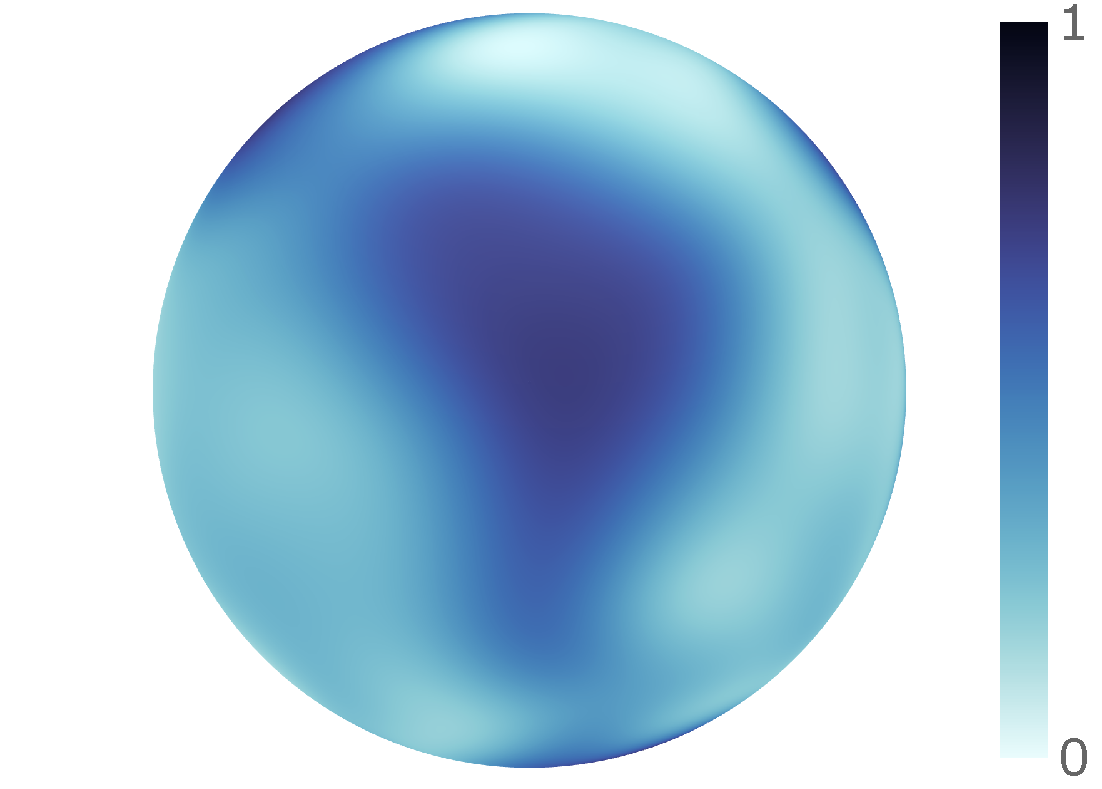
\includegraphics[trim={23 7 3 6},clip,width=.5\textwidth]{harmonic_gaussian_10lsig_10msig_L128_convolved_earth_L128_res512_real_norm.pdf}}
	\caption[
		Two harmonic Gaussians convolved with a map of the Earth
	]{
		The real part of the sifting convolution between the EGM2008 dataset and the harmonic Gaussian, rotated to view of South America (bandlimited at \(L=128\)).
		Panel (a) corresponds to a more elongated kernel \(f_{A}\), where \((\sigma_{\ell},\sigma_{m}) = (10^{2}, 10^{1})\); whereas panel (b) corresponds to a more symmetric kernel \(f_{B}\), where \((\sigma_{\ell},\sigma_{m}) = (10^{1}, 10^{1})\).
		As expected, the resultant sifting convolved Earth map exhibits greater anisotropic smoothing in panel (a) than in panel (b).
		It is clear that the sifting convolution supports directional kernels to perform anisotropic filtering (smoothing), while the output remains on the sphere.
		The colour is between zero and one, reflecting the scaled intensity of the field.
	}\label{fig:chapter2_convolved}
\end{figure}


\section{Conclusion}\label{sec:chapter2_conclusion}

This work presents the \emph{sifting convolution} on the sphere and demonstrates its application.
The convolution accepts directional functions as inputs, has an output which remains on the sphere, and is efficient to compute.
The sifting convolution is defined in the usual manner through the inner product but with an alternative translation operator on the sphere.
This follows by analogy with the Euclidean translation when viewed as a convolution with a shifted Dirac delta function.
An illustration of the sifting convolution on the topographic map of the Earth demonstrates that it supports directional kernels to perform anisotropic filtering, while its output remains on the sphere.
Convolutions are an important part of signal processing techniques, hence, the sifting convolution can play an integral role in constructions of alternate spherical analysis techniques, which is the focus of future work.

\chapter{Sifting Convolution on the Sphere}\label{sec:chapter3}

A novel spherical convolution is defined through the sifting property of the Dirac delta on the sphere.
The so-called sifting convolution is defined by the inner product of one function with a translated version of another, that follows by the adoption of an alternative translation operator on the sphere.
This translation operator follows by analogy with the Euclidean translation when viewed in harmonic space.
The sifting convolution satisfies a variety of desirable properties that are lacking in alternate definitions, namely: it supports directional kernels; it has an output which remains on the sphere; and, is efficient to compute.
An illustration of the sifting convolution on a topographic map of the Earth demonstrates that it supports directional kernels to perform anisotropic filtering, while its output remains on the sphere.
This chapter is adapted from~\cite{Roddy2021}, in which I was the lead author.

\section{Introduction}

Many fields in science and engineering measure data on spherical manifolds, such as computer graphics~\cite{Ramamoorthi2004}, planetary science~\cite{Turcotte1981}, geophysics~\cite{Simons2006}, quantum chemistry~\cite{Choi1999}, cosmology~\cite{Bennett1996}, and computer vision~\cite{Cohen2018,Esteves2020,Cobb2021}.
Possible extensions to signal processing techniques developed in the Euclidean domain may be transferred to the spherical domain.
The convolution is an important signal processing technique between two signals defined on the 2-sphere, which is central to filtering --- an integral part of spherical analyses.

Many definitions of spherical convolutions exist in the literature.
A spherical convolution operator would ideally exhibit a variety of desirable properties --- such a spherical convolution would accept directional inputs (\ie{} functions that are \emph{not} invariant under azimuthal rotation), whilst having the output remain on the sphere.
Moreover, the convolution would be efficient to compute.
Existing convolutions such as the isotropic convolution (\eg{}~\cite{McEwen2007,Wei2011,Kennedy2011}) and the left convolution~\cite{Kennedy2011,Driscoll1994} restrict themselves to an axisymmetric kernel (\ie{} kernels that are invariant under azimuthal rotation).
The directional convolution has an output which is not on the sphere (\eg{}~\cite{McEwen2007,Wandelt2001}).
Lastly, the commutative anisotropic convolution~\cite{Sadeghi2012,Khalid2012} and the directional convolution are computationally demanding.
No existing spherical convolution satisfies all three desirable properties.

This chapter presents an alternative spherical convolution, the sifting convolution, defined through the sifting property of the Dirac delta --- in analogy to the Euclidean definition.
The convolution is anisotropic in nature and supports directional kernels.
The output remains on the sphere, even when both inputs are directional.
Moreover, the convolution is efficient to compute, and is commutative up to a complex conjugate.

The remainder of this chapter is as follows.
\cref{sec:chapter3_preliminaries} includes some mathematical preliminaries and reviews existing spherical convolutions in the literature.
\cref{sec:chapter3_sifting_convolution} introduces the proposed sifting convolution.
\cref{sec:chapter3_numerical_illustration} presents a demonstration of the convolution with a directional kernel.
Lastly, \cref{sec:chapter3_conclusion} sets out some concluding remarks.

\section{Mathematical Background and Problem Formulation}\label{sec:chapter3_preliminaries}

\subsection{Mathematical Preliminaries}

A brief review of the mathematical preliminaries required for this chapter is presented here, for more detail see the relevant sections in \cref{sec:chapter2}.

\subsubsection{Signals on the Sphere}

Consider a complex valued square-integrable function \(\pixel{f}\) on the 2-sphere
%
\begin{equation}
	\twoSphere{}
	%
	= \set{\omega \in \mathbb{R}^{3} : \norm{\omega} = 1}.
\end{equation}
%
Here \(\omega=(\theta,\phi)\) parameterise a point on the unit sphere, where \(\theta \in \interval{0}{\pi}\) is the colatitude and \(\phi \in \interval[open right]{0}{2\pi}\) is the longitude.
The functions \(\pixel{f}\) form the Hilbert space \(\hilbert{\twoSphere}\).
The complex inner product induces a norm
%
\begin{equation}
	\norm{f}
	%
	= \sqrt{\braket*{f}}.
\end{equation}
%
Signals on the sphere are functions with a finite induced norm.

\subsubsection{Spherical Harmonics}

The spherical harmonics are the complete orthonormal set of basis functions of the Hilbert space \(\hilbert{\twoSphere}\)
%
\begin{equation}\label{eq:chapter3_spherical_harmonic}
	\pixel{\harmonic{Y}}
	%
	= \phaseFactor \sqrt{\factor \frac{(\ell-m)!}{(\ell+m)!}} P^{m}_{\ell}(\cos{\theta}) \exp(i m\phi),
\end{equation}
%
where \(P^{m}_{\ell}(x)\) are the associated Legendre polynomials.
By the completeness of spherical harmonics, any \(f \in \hilbert{\twoSphere}\) may be decomposed as
%
\begin{equation}
	\pixel{f}
	%
	= \sum\limits_{\ell=0}^{\infty} \sum\limits_{m=-\ell}^{\ell} \harmonic{f} \pixel{\harmonic{Y}},
\end{equation}
%
where \(\harmonic{f}\) are the spherical harmonic coefficients given by
%
\begin{equation}
	\harmonic{f}
	%
	= \integrateSphere{\omega} \pixel{f} \pixel{\conj{\harmonic{Y}}}.
\end{equation}
%
The phase convention adopted here is
%
\begin{equation}\label{eq:chapter3_spherical_harmonic_phase}
	\pixel{\conj{\harmonic{Y}}}
	%
	= \phaseFactor \pixel{Y_{\ell(-m)}},
\end{equation}
%
such that
%
\begin{equation}
	\conj{\harmonic{f}}
	%
	= \phaseFactor f_{\ell(-m)}
\end{equation}
%
for a real field.
One often considers signals on the sphere with a bandlimit of \(L\), \ie{} signals such that \(\harmonic{f} = 0,\ \forall \ell \geq L\), and adopts the shorthand notation
%
\begin{equation}
	\harmonicSum
	%
	= \sum\limits_{\ell=0}^{L-1} \sum\limits_{m=-\ell}^{\ell}.
\end{equation}

\subsubsection{Dirac Delta}

In harmonic space the Dirac delta on the sphere rotated to some \(\omega'=(\theta',\phi')\) is
%
\begin{equation}
	\pixel{\delta_{\omega'}}
	%
	= \harmonicSum \pixel[']{\conj{\harmonic{Y}}} \pixel{\harmonic{Y}},
\end{equation}
%
which can be shown to be real
%
\begin{align}\label{eq:chapter3_dirac_delta_real}
	\pixel{\delta_{\omega'}}
	%
	 & = \harmonicSum \pixel[']{\conj{\harmonic{Y}}} \pixel{\harmonic{Y}} \nonumber{}                           \\
	%
	 & = \harmonicSum \phaseFactor \pixel[']{Y_{\ell(-m)}} \phaseFactor \pixel{\conj{Y_{\ell(-m)}}} \nonumber{} \\
	%
	 & = \sum\limits_{\ell m'} \pixel[']{Y_{\ell m'}} \pixel{\conj{Y_{\ell m'}}} \nonumber{}                    \\
	%
	 & = \pixel{\conj{\delta_{\omega'}}},
\end{align}
%
where the second line follows by \cref{eq:chapter3_spherical_harmonic_phase}.
The Dirac delta on the sphere is normalised
%
\begin{equation}
	\integrateSphere{\omega} \pixel{\delta_{\omega'}}
	%
	= 1,
\end{equation}
%
as
%
\begin{align}
	\integrateSphere{\omega} \pixel{\delta_{\omega'}}
	%
	 & = \integrateSphere{\omega} \harmonicSum \pixel[']{\conj{\harmonic{Y}}} \pixel{\harmonic{Y}} \nonumber{}                            \\
	%
	 & = \harmonicSum \pixel[']{\conj{\harmonic{Y}}} \integrateSphere{\omega} \pixel{\harmonic{Y}} \pixel{Y_{00}} \sqrt{4\pi} \nonumber{} \\
	%
	 & = \sqrt{4\pi} \harmonicSum \pixel[']{\conj{\harmonic{Y}}} \delta_{\ell0} \delta_{m0} \nonumber{}                                   \\
	%
	 & = \sqrt{4\pi} \pixel[']{\conj{Y_{00}}} \nonumber{}                                                                                 \\
	%
	 & = 1,
\end{align}
%
where the second and third lines follow by substituting \(\sqrt{4\pi}\pixel{Y_{00}}=1\) (\cf{} \cref{eq:chapter3_spherical_harmonic}) and the orthonormality of the spherical harmonics respectively.
The sifting property of the Dirac delta is
%
\begin{equation}
	\integrateSphere{\omega} \pixel{\delta_{\omega'}} \pixel{f}
	%
	= \pixel[']{f},
\end{equation}
%
as
%
\begin{align}
	\integrateSphere{\omega} \pixel{\delta_{\omega'}} \pixel{f}
	%
	 & = \integrateSphere{\omega} \pixel{\conj{\delta_{\omega'}}} \pixel{f} \nonumber{}                                                                                \\
	%
	 & = \integrateSphere{\omega} \harmonicSum \pixel[']{\harmonic{Y}} \pixel{\conj{\harmonic{Y}}} \harmonicSum['] \harmonic[']{f} \pixel{\harmonic[']{Y}} \nonumber{} \\
	%
	 & = \harmonicSum \harmonic{f} \pixel[']{\harmonic{Y}} \nonumber{}                                                                                                 \\
	%
	 & = \pixel[']{f},
\end{align}
%
where the first line holds due to the reality of the Dirac delta \cref{eq:chapter3_dirac_delta_real}.

\subsubsection{Rotation of a Signal on the 2-Sphere}

The Euler angles may parameterise three-dimensional rotations with \(\rho = (\alpha,\beta,\gamma) \in \rotationGroup{}\), where \(\alpha \in \interval[open right]{0}{2\pi}\), \(\beta \in \interval{0}{\pi}\), and \(\gamma \in \interval[open right]{0}{2\pi}\).
The rotation operator \(\rotation{\rho}\) consists of the sequence of rotations:
%
\begin{enumerate}[(i),nosep,left=\parindent]
	\item \({\gamma}\) rotation about the \(z\)-axis;
	\item \({\beta}\) rotation about the \(y\)-axis; and
	\item \({\alpha}\) rotation about the \(z\)-axis.
\end{enumerate}
%
The rotation of a function on the sphere is defined by
%
\begin{equation}\label{eq:chapter3_rotation_matrix}
	\pixel{(\rotation{\rho}f)}
	%
	= f(\rotationMatrix^{-1} \omega),
\end{equation}
%
where \(\rotationMatrix{}\) is the three-dimensional rotation matrix corresponding to \(\rotation{\rho}\).
The spherical harmonic coefficients of a rotated function read
%
\begin{equation}\label{eq:chapter3_rotation_operator}
	\harmonic{(\rotation{\rho}f)}
	%
	= \wignerSum \wigner{\ell}{m}{n}(\rho) f_{\ell n},
\end{equation}
%
where \(\wigner{\ell}{m}{n}(\rho)\) are Wigner D matrices given by
%
\begin{equation}
	\wigner{\ell}{m}{n}(\rho)
	%
	= \exp(-i m\alpha) \reducedWigner{\ell}{m}{n}(\beta) \exp(-i n\gamma),
\end{equation}
%
which form the \(2\ell+1\)-dimensional representation of the rotation group for a given \(\ell{}\).
The \(\reducedWigner{\ell}{m}{n}(\beta)\) are the reduced d matrices, which are real in this phase convention and satisfy many symmetry relations.
Note the proportionality of the axisymmetric rotation matrices and the spherical harmonics
%
\begin{equation}\label{eq:chapter3_wigner_axisymmetric}
	\wigner[\ast]{\ell}{m}{0}(\phi,\theta,0)
	%
	= \sqrt{\inverseFactor} \pixel{\harmonic{Y}}.
\end{equation}

\subsection{Spherical Convolutions}\label{sec:chapter3_spherical_convolutions}

The conventional convolution between two functions on two-dimensional Euclidean space \(\mathbb{R}^{n}\) is
%
\begin{equation}
	(f \star g)(x)
	%
	= \int\limits_{\mathbb{R}^{2}} \dd{y} f(x-y) g(y),
\end{equation}
%
where \(x,\ y \in \mathbb{R}^{n}\).
The convolution is commutative
%
\begin{equation}
	f \star g
	%
	= g \star f.
\end{equation}
%
A spherical counterpart of the convolution is required for functions defined on the sphere.
Alternative definitions of such a convolution exist in the literature but, while already useful, lack certain desirable properties.
The properties desired in the spherical extension of the convolution include:
%
\begin{enumerate}[(i),nosep,left=\parindent]
	\item the support of directional kernels;
	\item an output which remains on the sphere; and
	\item efficient computation.
\end{enumerate}
%
A convolution is considered computationally efficient here if its computational cost is no greater than the cost of fast spherical harmonic transforms, \ie{} \(\mathcal{O}(L^{3})\) (\eg{}~\cite{Driscoll1994,McEwen2011}).
Formulations of spherical convolutions exist in the literature, but none satisfy all properties.
A summary of existing spherical convolutions and their properties follows.

\subsubsection{Isotropic Convolution}

In real space the isotropic convolution (\eg{}~\cite{McEwen2007,Wei2011,Kennedy2011}) is
%
\begin{equation}
	\pixel{(f \odot g)}
	%
	= \integrateSphere{\omega'} \pixel[']{f} \pixel[']{\conj{(\rotation{\omega}g)}},
\end{equation}
%
which in harmonic space becomes (\eg{}~\cite{McEwen2007})
%
\begin{equation}\label{eq:chapter3_isotropic_harmonic}
	\harmonic{(f \odot g)}
	%
	= \sqrt{\inverseFactor} \harmonic{f} \conj{\axiHarmonic{g}},
\end{equation}
%
as
%
\begin{align}
	\pixel{(f \odot g)}
	%
	 & = \integrateSphere{\omega'} \pixel[']{f} \pixel[']{\conj{(\rotation{\omega}g)}} \nonumber{}                                                                                           \\
	%
	 & = \integrateSphere{\omega'} \harmonicSum \harmonic{f} \pixel[']{\harmonic{Y}} \harmonicSum['] \conj{\harmonic[']{(\rotation{\omega}g)}} \pixel[']{\conj{\harmonic[']{Y}}} \nonumber{} \\
	%
	 & = \harmonicSum \harmonic{f} \conj{\harmonic{(\rotation{\omega}g)}} \nonumber                                                                                                          \\
	%
	 & = \harmonicSum \harmonic{f} \conj{\big(\wigner{\ell}{m}{0}(\phi,\theta,0) \axiHarmonic{g}\big)} \nonumber{}                                                                           \\
	%
	 & = \harmonicSum \sqrt{\inverseFactor} \harmonic{f} \conj{\axiHarmonic{g}} \pixel{\harmonic{Y}},
\end{align}
%
where the last line follows by \cref{eq:chapter3_wigner_axisymmetric}.
The isotropic convolution has the following properties:
%
\begin{enumerate}[(i),nosep,left=\parindent]
	\item does not support directional kernels since \(\pixel{g}\) must be axisymmetric;
	\item an output which remains on the sphere; and
	\item efficient computation since it is a product in harmonic space.
\end{enumerate}

\subsubsection{Left Convolution}

The definition of the left convolution~\cite{Kennedy2011,Driscoll1994} in real space is
%
\begin{equation}
	\pixel{(f \circleddash g)}
	%
	= \integrateRotation{\rho} f(\rotationMatrix\eta) g(\rotationMatrix^{-1}\omega),
\end{equation}
%
where \({\eta}\) is the north pole, and \(\rotationVolume=\sin{\beta} \dd{\alpha} \dd{\beta} \dd{\gamma}\) is the usual invariant measure on \(\rotationGroup{}\).
The harmonic representation of this convolution is
%
\begin{equation}
	\harmonic{(f \circleddash g)}
	%
	= 2\pi \sqrt{\inverseFactor} \harmonic{f} \axiHarmonic{g}.
\end{equation}
%
To prove this, first consider the forward harmonic transform
%
\begin{align}
	\harmonic{(f \circleddash g)}
	%
	 & = \integrateSphere{\omega} \integrateRotation{\rho} f(\rotationMatrix\eta) g(\rotationMatrix^{-1}\omega) \pixel{\conj{\harmonic{Y}}} \nonumber{}                                            \\
	%
	 & = \integrateRotation{\rho} f(\rotationMatrix\eta) \integrateSphere{\omega} \pixel{(\rotation{\rho}g)} \pixel{\conj{\harmonic{Y}}} \nonumber{}                                               \\
	%
	 & = \integrateRotation{\rho} f(\rotationMatrix\eta) \integrateSphere{\omega} \harmonicSum['] \harmonic[']{(\rotation{\rho}g)} \pixel{\harmonic[']{Y}} \pixel{\conj{\harmonic{Y}}} \nonumber{} \\
	%
	 & = \integrateRotation{\rho} f(\rotationMatrix\eta) \harmonic{(\rotation{\rho}g)} \nonumber{}                                                                                                 \\
	%
	 & = \wignerSum g_{\ell n} \integrateRotation{\rho} f(\rotationMatrix\eta) \wigner{\ell}{m}{n}(\rho),
\end{align}
%
where the second and last line follow by \cref{eq:chapter3_rotation_operator,eq:chapter3_rotation_matrix} respectively.
Due to the invariant measure \(\rotationVolume{}\) and considering a right rotation about the \(z\)-axis by \({\chi}\), \ie{} \(\rho = (\alpha,\beta,\gamma) \rightarrow \rho' = (\alpha,\beta,\gamma+\chi)\), it follows
%
\begin{align}\label{eq:chapter3_so3_integral}
	\integrateRotation{\rho} f(\rotationMatrix\eta) \wigner{\ell}{m}{n}(\rho)
	%
	 & = \integrateRotation{\rho} f(\rotationMatrix[']\eta) \wigner{\ell}{m}{n}(\rho') \nonumber{}            \\
	%
	 & = \integrateRotation{\rho} f(\rotationMatrix\eta) \exp(-i n\chi) \wigner{\ell}{m}{n}(\rho) \nonumber{} \\
	%
	 & = \exp(-i n\chi) \integrateRotation{\rho} f(\rotationMatrix\eta) \wigner{\ell}{m}{n}(\rho),
\end{align}
%
where the penultimate line follows since a rotation of \({\eta}\) about the \(z\)-axis leaves \({\eta}\) unchanged, \ie{} \(f(\rotationMatrix[']\eta) = f(\rotationMatrix\eta)\).
Thus, as \cref{eq:chapter3_so3_integral} holds for all \(\chi{}\), it must be the case that \(n=0\) unless the integral is zero, \ie{}
%
\begin{align}
	\harmonic{(f \circleddash g)}
	%
	 & = \axiHarmonic{g} \integrateRotation{\rho} f(\rotationMatrix\eta) \wigner{\ell}{m}{0} (\alpha,\beta,0) \nonumber{}                                    \\
	%
	 & = \axiHarmonic{g} \int\limits_{0}^{2\pi} \dd{\gamma} \integrateSphere{\omega} \pixel{f} \sqrt{\inverseFactor} \pixel{\conj{\harmonic{Y}}} \nonumber{} \\
	%
	 & = 2\pi \sqrt{\inverseFactor} \harmonic{f} \axiHarmonic{g},
\end{align}
%
where the penultimate line follows by \cref{eq:chapter3_wigner_axisymmetric}.
As the harmonic representations suggest, the isotropic and left convolutions are closely related, as elaborated in~\cite{Kennedy2011}.
Hence, the properties are similar.
The left convolution has the following properties:
%
\begin{enumerate}[(i),nosep,left=\parindent]
	\item does not support directional kernels since \(\pixel{g}\) must be axisymmetric;
	\item an output which remains on the sphere; and
	\item efficient computation since it is a product in harmonic space.
\end{enumerate}

\subsubsection{Directional Convolution}

Rotations on the sphere are the spherical counterpart of translations in the Euclidean domain in real space.
Hence, the standard directional convolution is
%
\begin{equation}\label{eq:chapter3_directional_convolution}
	(f \circledast g)(\rho)
	%
	= \integrateSphere{\omega} \pixel{f} \pixel{\conj{(\rotation{\rho}g)}}.
\end{equation}
%
Upon expanding in harmonic space, this becomes (\eg{}~\cite{McEwen2007,Wandelt2001})
%
\begin{equation}
	(f \circledast g) (\rho)
	%
	= \harmonicSum \harmonic{f} \wignerSum \conj{\big(\wigner{\ell}{m}{n}(\rho) g_{\ell n}\big)},
\end{equation}
%
as
%
\begin{align}
	(f \circledast g)(\rho)
	%
	 & = \integrateSphere{\omega} \pixel{f} \pixel{\conj{(\rotation{\rho}g)}} \nonumber{}                                                                                           \\
	%
	 & = \integrateSphere{\omega} \harmonicSum \harmonic{f} \pixel{\harmonic{Y}} \harmonicSum['] \conj{\harmonic[']{(\rotation{\rho}g)}} \pixel{\conj{\harmonic[']{Y}}} \nonumber{} \\
	%
	 & = \harmonicSum \harmonic{f} \conj{\harmonic{(\rotation{\rho}g)}} \nonumber{}                                                                                                 \\
	%
	 & = \harmonicSum \harmonic{f} \wignerSum \conj{\big(\wigner{\ell}{m}{n}(\rho) g_{\ell n}\big)},
\end{align}
%
and hence, the output is on \(\rotationGroup{}\).
Fast algorithms exist~\cite{McEwen2007,Wandelt2001,Wiaux2007,McEwen2013}, but the convolution remains less efficient than a spherical harmonic transform.
The directional convolution has the following properties:
%
\begin{enumerate}[(i),nosep,left=\parindent]
	\item does support directional kernels;
	\item an output which does not remain on the sphere due to the three-dimensional rotation of the kernel; and
	\item expensive computation.
\end{enumerate}

\subsubsection{Commutative Anisotropic Convolution}

The definition of the commutative anisotropic convolution~\cite{Sadeghi2012,Khalid2012} is
%
\begin{equation}
	\pixel{(f \oplus g)}
	%
	= \integrateSphere{\omega'} \pixel[']{(\rotation{(\phi,\theta,\pi-\phi)}f)} \pixel[']{g},
\end{equation}
%
which on expansion reads
%
\begin{equation}
	\pixel{(f \oplus g)}
	%
	= \harmonicSum \wignerSum \wigner{\ell}{m}{n}(\phi,\theta,\pi-\phi) f_{\ell n} \conj{\harmonic{g}},
\end{equation}
%
as
%
\begin{align}
	\pixel{(f \oplus g)}
	%
	 & = \integrateSphere{\omega'} \pixel[']{(\rotation{(\phi,\theta,\pi-\phi)}f)} \pixel[']{g} \nonumber{}                                                                                                  \\
	%
	 & = \integrateSphere{\omega'} \harmonicSum \harmonic{(\rotation{(\phi,\theta,\pi-\phi)}f)} \pixel[']{\harmonic{Y}} \harmonicSum['] \conj{\harmonic[']{g}} \pixel[']{\conj{\harmonic[']{Y}}} \nonumber{} \\
	%
	 & = \harmonicSum \harmonic{(\rotation{(\phi,\theta,\pi-\phi)}f)} \conj{\harmonic{g}} \nonumber{}                                                                                                        \\
	%
	 & = \harmonicSum \wignerSum \wigner{\ell}{m}{n}(\phi,\theta,\pi-\phi) f_{\ell n} \conj{\harmonic{g}}.
\end{align}
%
The limitation here is that one must specify the initial rotation as \({\gamma=\pi-\alpha}\) in order for the convolution to be commutative.
The complexity of the convolution is \(\mathcal{O}(L^{3}\log{L})\), and hence, it is less efficient than a spherical harmonic transform.
The convolution has the following properties:
%
\begin{enumerate}[(i),nosep,left=\parindent]
	\item it supports directional kernels;
	\item an output which remains on the sphere; and
	\item expensive computation.
\end{enumerate}

\subsection{Problem Formulation}

\cref{tab:chapter3_properties} presents a summary of the spherical convolutions discussed and their properties.
No existing definition of a spherical convolution has all the desired properties discussed in \cref{sec:chapter3_spherical_convolutions}.
In this chapter, the sifting convolution, which satisfies all desirable properties, is presented.

\begin{table}
	\centering
	\caption[
		Properties of spherical convolutions
	]{
		Properties of spherical convolutions.
	}\label{tab:chapter3_properties}
	\begin{tabular}{@{}rccc@{}}
		\toprule
		                        & Anisotropic & \(\twoSphere{}\) Output & Efficient \\
		\midrule
		Isotropic               & \ding{55}   & \ding{51}               & \ding{51} \\
		%
		Left                    & \ding{55}   & \ding{51}               & \ding{51} \\
		%
		Directional             & \ding{51}   & \ding{55}               & \ding{55} \\
		%
		Commutative Anisotropic & \ding{51}   & \ding{51}               & \ding{55} \\
		%
		Sifting (this work)     & \ding{51}   & \ding{51}               & \ding{51} \\
		\bottomrule
	\end{tabular}
\end{table}


\section{Sifting Convolution}\label{sec:chapter3_sifting_convolution}

This chapter defines the sifting convolution which permits directional kernels, whose output remains on the sphere and is efficient to compute.
Moreover, it is commutative up to a complex conjugate.
The sifting convolution is constructed using a novel translation operator defined on the sphere.

\subsection{Translation Operator}\label{sec:chapter3_translation_operator}

In real space, the rotation operator on the sphere is the usual analogue of the translation operator in the Euclidean setting.
One may define an alternative operator, \(\translation{\omega}\), which follows as the analogue of the Euclidean setting but in harmonic space.
This translation is in contrast to the standard rotation as it considers two angles rather than three and thereby its output remains on the sphere.
In practice the translation operator is defined as a product of basis functions.
In the Euclidean setting, \eg{} \(\mathbb{R}\), the complex exponentials
%
\begin{equation}\label{eq:chapter3_complex_exponentials}
	\zeta_{u}(x)
	%
	= \exp(i u x),
\end{equation}
%
with \(x,\ u \in \mathbb{R}\) form the standard orthonormal basis.
A shift of coordinates defines the translation of the basis functions
%
\begin{equation}\label{eq:chapter3_exponentials_shift}
	\zeta_{u}(x + y)
	%
	= \zeta_{u}(y) \zeta_{u}(x),
\end{equation}
%
with \(y \in \mathbb{R}\) and where the final equality follows by the standard rule for exponents.
The definition of the translation of the spherical harmonics on the sphere follows by analogy with the representation as a product of basis functions
%
\begin{equation}\label{eq:chapter3_translation_basis_functions}
	\pixel{(\translation{\omega'}\harmonic{Y})}
	%
	\equiv \pixel[']{\harmonic{Y}} \pixel{\harmonic{Y}},
\end{equation}
%
where \(\omega'=(\theta',\phi')\).

This leads to a natural harmonic expression for the translation of a general arbitrary function \(f \in \hilbert{\twoSphere}\)
%
\begin{equation}\label{eq:chapter3_translation_real}
	\pixel{(\translation{\omega'}f)}
	%
	= \harmonicSum \harmonic{f} \pixel[']{\harmonic{Y}} \pixel{\harmonic{Y}},
\end{equation}
%
implying
%
\begin{equation}\label{eq:chapter3_translation_harmonic}
	\harmonic{(\translation{\omega'}f)}
	%
	= \harmonic{f} \pixel[']{\harmonic{Y}}.
\end{equation}
%
This translation operator is considered further in \cref{sec:chapter3_translation_interpretation} to build greater intuition.

\subsection{Convolution Operator}

With a translation operator to hand, one may define the sifting convolution on the sphere of \(f,\ g \in \hilbert{\twoSphere}\) in the usual manner by the inner product
%
\begin{equation}\label{eq:chapter3_convolution_real}
	\pixel{\convolution{f}{g}}
	%
	\equiv \braket*{\translation{\omega}f}{g},
\end{equation}
%
noting the use of the alternative translation operator defined in \cref{sec:chapter3_translation_operator}.
In harmonic space this simplifies to the product
%
\begin{equation}\label{eq:chapter3_convolution_harmonic}
	\harmonic{\convolution{f}{g}}
	%
	= \harmonic{f} \conj{\harmonic{g}},
\end{equation}
%
as
%
\begin{align}
	\pixel{(f \circledcirc g)}
	%
	 & = \braket*{\translation{\omega}f}{g} \nonumber{}                                                                                                                                        \\
	%
	 & = \integrateSphere{\omega'} \pixel[']{(\translation{\omega}f)} \pixel[']{\conj{g}} \nonumber{}                                                                                          \\
	%
	 & = \integrateSphere{\omega'} \harmonicSum \harmonic{f} \pixel[']{\harmonic{Y}} \pixel{\harmonic{Y}} \harmonicSum['] \conj{\harmonic[']{g}} \pixel[']{\conj{\harmonic[']{Y}}} \nonumber{} \\
	%
	 & = \harmonicSum \harmonic{f} \conj{\harmonic{g}} \pixel{\harmonic{Y}}.
\end{align}
%
Since the harmonic representation of the convolution is simply a product (again by analogy with the harmonic representation of the Euclidean convolution), it is efficient to compute.
Note that harmonic multiplication has been considered before~\cite{Kennedy2011}; although it has been used here to define a new anisotropic convolution operator, introducing a conjugation and elaborating a real space interpretation.

\subsection{Translation Interpretation}\label{sec:chapter3_translation_interpretation}

One may show that the translation operator is simply a (sifting) convolution of a function with the shifted Dirac delta function
%
\begin{align}
	\pixel{\convolution{f}{\delta_{\omega'}}}
	%
	 & = \harmonicSum \harmonic{f} \pixel[']{\harmonic{Y}} \pixel{\harmonic{Y}} \nonumber{} \\
	%
	 & = \pixel{(\translation{\omega'}f)},
\end{align}
%
by noting \cref{eq:chapter3_convolution_harmonic} and where the final equality follows by \cref{eq:chapter3_translation_real}.
The sifting convolution and translation are thus natural analogues of the respective operators defined in Euclidean space.

\subsection{Properties}\label{sec:chapter3_properties}

The sifting convolution has all the desired properties discussed in \cref{sec:chapter3_spherical_convolutions}, namely, the convolution accepts directional inputs, has an output which remains on the sphere, and is efficient to compute.
\cref{tab:chapter3_properties} summarises the properties of the sifting convolution and compares them to the properties of alternative spherical convolutions.

The translation preserves symmetries, which means that any symmetry that exists in the initial kernel definition will be present after the translation.
Thus, one must be careful when choosing a kernel for a convolution to ensure that it has the desired properties when translated, \eg{} spatial localisation.
To perform anisotropic smoothing that is localised (the usual interpretation), the translated kernel also needs to be localised.
If the kernel has, say, even azimuthal symmetry, when it is translated to \(\omega'=(\theta', \phi')\) it will have a localised component both at \(\phi'\) and \(-\phi'\).
While this is not a problem \emph{per se}, for the usual interpretation of smoothing one would desire a localised component at \(\phi'\) only.
This can be achieved by ensuring that the original kernel does not exhibit a symmetry that would lead to multiple localised components once translated.
The harmonic Gaussian introduced in \cref{sec:chapter3_numerical_illustration} satisfies the desired property.

\section{Numerical Illustration}\label{sec:chapter3_numerical_illustration}

This section demonstrates the effect of the sifting convolution through the application of a directional kernel to an example signal on the sphere.
Some potential kernels are defined in \cref{sec:chapter3_kernels}, where the effect of the translation is explored.
The convolution is then demonstrated with one of these kernels in \cref{sec:chapter3_convolution} on a topographic map of the Earth.
All later computations use the \texttt{SSHT}\footnote{\url{http://astro-informatics.github.io/ssht/}} code~\cite{McEwen2011}.

\subsection{Kernels}\label{sec:chapter3_kernels}

As discussed in \cref{sec:chapter3_properties}, the translation preserves symmetries from the initial kernel definition.
Hence, one must consider the desired properties in the translated kernel, \eg{} spatial localisation.

\subsubsection{Gaussian}

First, consider the standard axisymmetric Gaussian on the sphere, \ie{}
%
\begin{equation}
	\harmonic{\mathcal{G}}
	%
	= \exp(-\frac{{\ell}^{2}}{2\sigma^{2}}),
\end{equation}
%
where \(\sigma{}\) is the standard deviation of the Gaussian.
\cref{fig:chapter3_gaussian} presents the Gaussian kernel (left panel) and the result of the translation (right panel); where it is clear that the axisymmetric symmetry is preserved.
This function has no directional components and is therefore only useful for some convolution purposes.

\begin{figure}[htpb]
	\centering\capstart{}
	\subfloat[\(\Re\big\{\pixel{\mathcal{G}}\big\}\)]{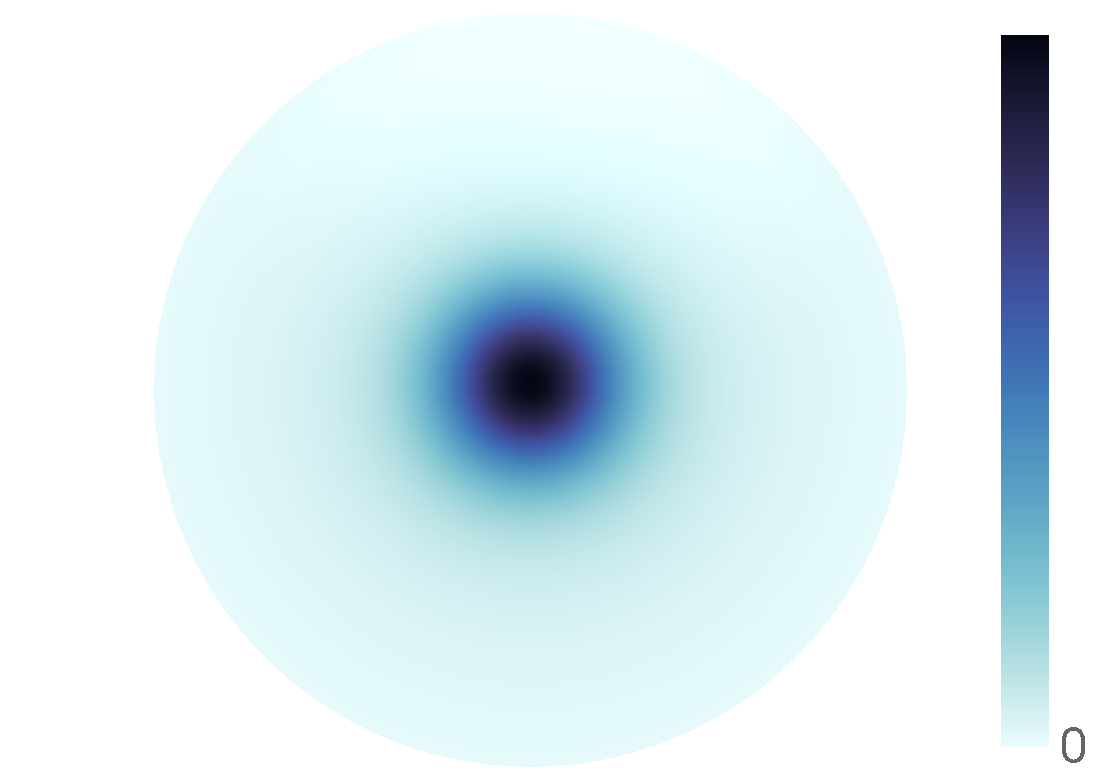
\includegraphics[trim={23 7 3 6},clip,width=.5\textwidth]{gaussian_10sig_L128_res512_real_norm.pdf}}
	\hfill
	\subfloat[\(\Re\big\{\pixel{(\translation{\omega'}\mathcal{G})}\big\}\)]{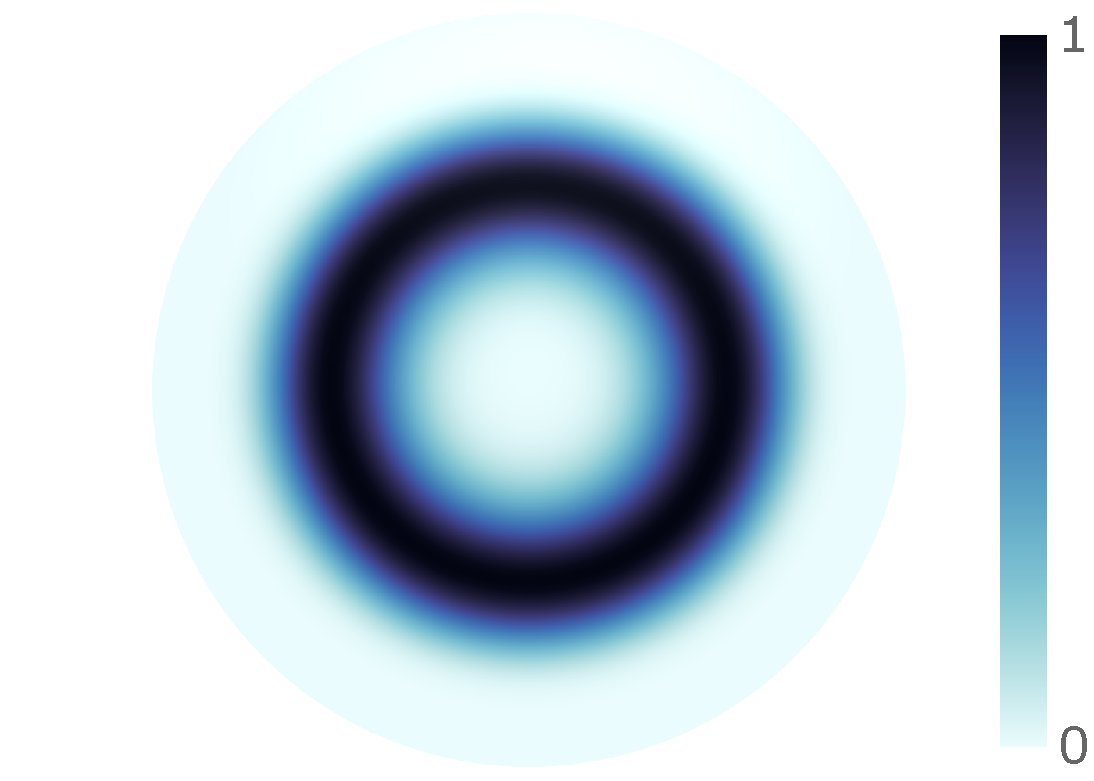
\includegraphics[trim={23 7 3 6},clip,width=.5\textwidth]{gaussian_10sig_L128_translate_alpha3pi4_beta1pi8_res512_real_norm.pdf}}
	\caption[
		A Gaussian on the north pole and then translated
	]{
		Panel (a) presents the standard axisymmetric Gaussian on the north pole (bandlimited at \(L=128\)).
		The Gaussian is then translated to some \(\omega'=(\theta',\phi')\), as shown in panel (b).
		Plainly, the axisymmetric symmetry has been preserved under translation.
		The colour is between zero and one, reflecting the scaled intensity of the field.
	}\label{fig:chapter3_gaussian}
\end{figure}


\subsubsection{Squashed Gaussian}

Define the squashed Gaussian in real space as the standard Gaussian (\ie{} in the polar angle \(\theta{}\)) modulated by a sinusoidal function in the azimuthal angle \(\phi{}\) by
%
\begin{equation}
	\pixel{\mathcal{SG}}
	%
	= \exp\Bigg(-\frac{1}{2}{\bigg(\frac{\theta-\mean{\theta}}{\sigma_{\theta}}\bigg)}^{2}\Bigg)
	%
	\sin{(\nu_{\phi}\phi)},
\end{equation}
%
where \(\mean{\theta}\)/\(\sigma_{\theta}\) and \(\nu_{\phi}\) are parameters controlling the mean/standard deviation of the Gaussian and the frequency of the sine wave respectively.
The squashed Gaussian kernel is shown in the left panel of \cref{fig:chapter3_squashed_gaussian}, and the translated kernel is shown in the right panel.
Under translation, the odd symmetry in the kernel definition is preserved; and hence, the squashed Gaussian is not suitable for smoothing purposes.

\begin{figure}[htpb]
	\centering\capstart{}
	\subfloat[\(\Re\big\{\pixel{\mathcal{SG}}\big\}\)]  % chktex 21
	{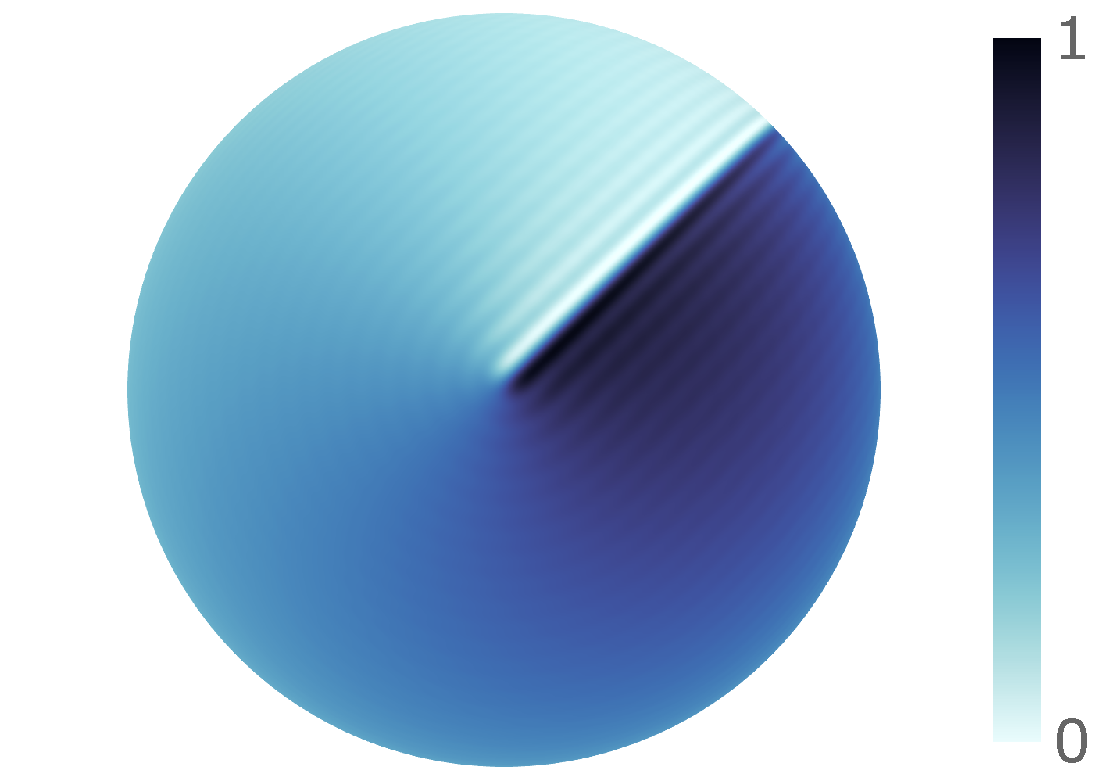
\includegraphics[trim={4 7 3 6},clip,width=.5\textwidth]{squashed_gaussian_1tsig_1freq10_L128_res512_real_norm.pdf}}
	\hfill
	\subfloat[\(\Re\big\{\pixel{(\translation{\omega'}\mathcal{SG})}\big\}\)]  % chktex 21
	{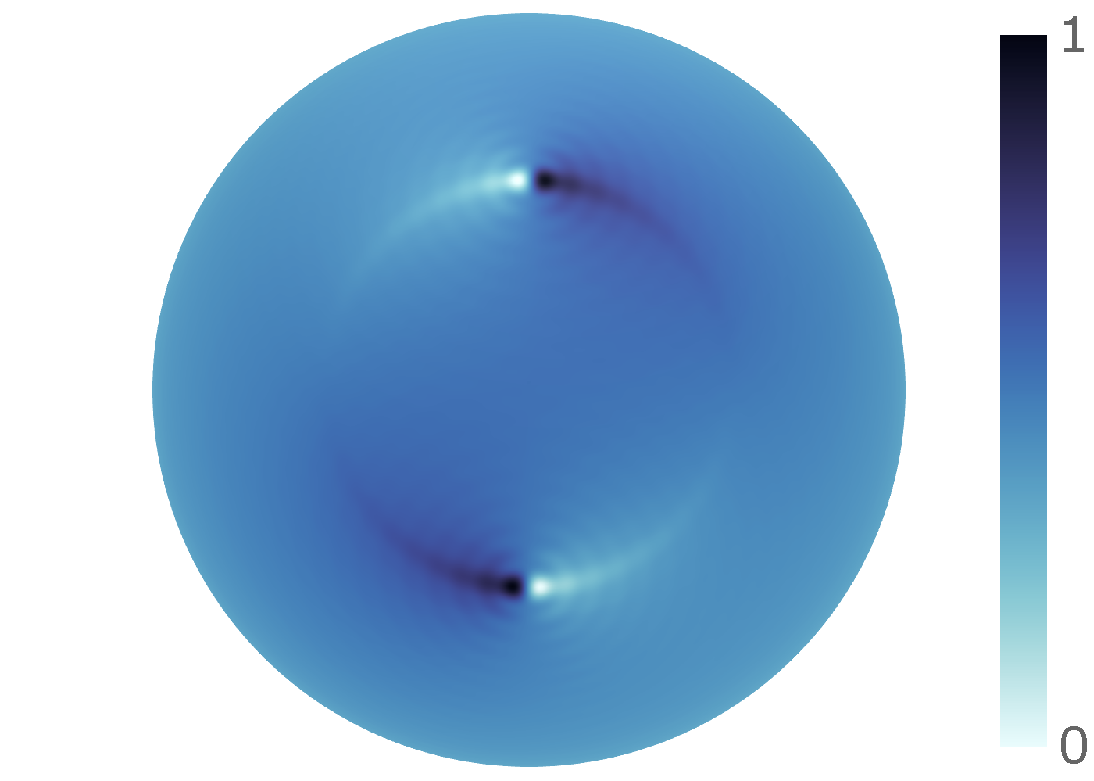
\includegraphics[trim={4 7 3 6},clip,width=.5\textwidth]{squashed_gaussian_1tsig_1freq10_L128_translate_alpha3pi4_beta1pi8_res512_real_norm.pdf}}
	\caption[
		A squashed Gaussian on the north pole and then translated
	]{
		Panel (a) presents the squashed Gaussian on the north pole (bandlimited at \(L=128\)).
		The squashed Gaussian is then translated to some \(\omega'=(\theta',\phi')\), as shown in panel (b).
		The odd azimuthal symmetry in the initial kernel definition is preserved under translation.
		The colour is between zero and one, reflecting the scaled intensity of the field.
	}\label{fig:chapter3_squashed_gaussian}
\end{figure}


\subsubsection{Elongated Gaussian}

Define the elongated Gaussian as a two-dimensional Gaussian in real space in the polar angle \(\theta{}\) and the azimuthal angle \(\phi{}\) by
%
\begin{equation}
	\pixel{\mathcal{EG}}
	%
	= \exp\bigg(-\bigg(\frac{{(\theta-\mean{\theta})}^{2}}{2\sigma_{\theta}^{2}}
		%
		+ \frac{{(\phi-\mean{\phi})}^{2}}{2\sigma_{\phi}^{2}}\bigg)\bigg),
\end{equation}
%
where \((\mean{\theta},\mean{\phi})\) are the means, and \((\sigma_{\theta},\sigma_{\phi})\) are the standard deviations of the respective Gaussians.
The left panel of \cref{fig:chapter3_elongated_gaussian} presents the elongated Gaussian, and the right panel shows the result of the translation.
The elongated Gaussian has even azimuthal symmetry which results in two localised components at \(\phi'\) and \(-\phi'\) upon translation.
Thus, this kernel is not suitable for anisotropic smoothing.

\begin{figure}[htpb]
	\centering\capstart{}
	\subfloat[\(\Re{\pixel{\mathcal{EG}}}\)]{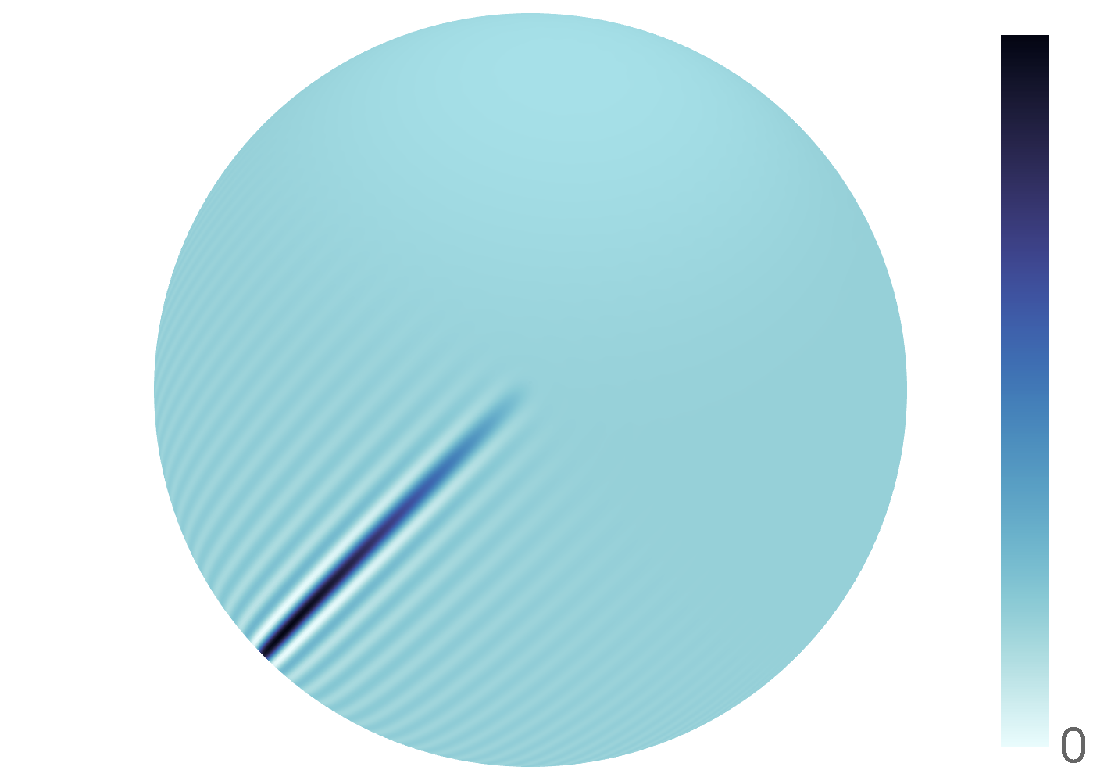
\includegraphics[trim={23 7 3 6},clip,width=.5\textwidth]{elongated_gaussian_1tsig_1psig1000_L128_res512_real_norm.pdf}}
	\hfill
	\subfloat[\(\Re{\pixel{(\translation{\omega'}\mathcal{EG})}}\)]{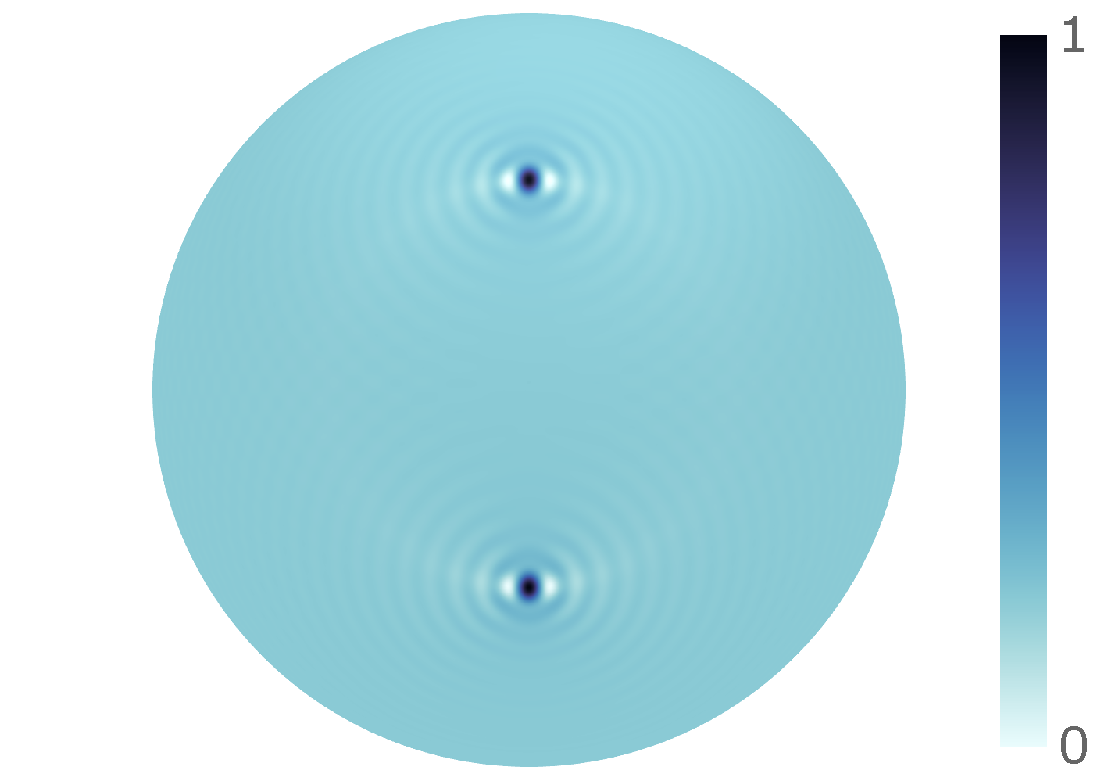
\includegraphics[trim={23 7 3 6},clip,width=.5\textwidth]{elongated_gaussian_1tsig_1psig1000_L128_translate_alpha3pi4_beta1pi8_res512_real_norm.pdf}}
	\caption[
		An elongated Gaussian on the north pole and then translated
	]{
		Panel (a) presents the elongated Gaussian on the north pole (bandlimited at \(L=128\)) --- where the central bar in the plot extends over half of the sphere.
		The elongated Gaussian is then translated to some \(\omega'=(\theta',\phi')\), as shown in panel (b).
		The even azimuthal symmetry in the initial kernel definition results into the two localised components at \(\phi'\) and \(-\phi'\) under translation.
		The colour is between zero and one, reflecting the scaled intensity of the field.
	}\label{fig:chapter3_elongated_gaussian}
\end{figure}


\subsubsection{Harmonic Gaussian}

Define the harmonic Gaussian as a two-dimensional Gaussian in harmonic space by
%
\begin{equation}\label{eq:chapter3_harmonic_gaussian}
	\harmonic{f}
	%
	= \exp(-\bigg(\frac{{\ell}^{2}}{2\sigma_{\ell}^{2}} + \frac{{m}^{2}}{2\sigma_{m}^{2}}\bigg)).
\end{equation}
%
In effect, this function is the standard axisymmetric Gaussian in \(\ell{}\) modulated by a Gaussian in \(m\).
Note this function is not real --- if required one can define only the positive \(m\) components and impose reality by the conjugate symmetry relationship in harmonic space.
The function is directional, and hence, is useful in illustrating the effect of the sifting convolution on the sphere.
Consider two differently sized harmonic Gaussians on the sphere to see the effect on the sifting convolution.
\cref{fig:chapter3_harmonic_gaussian} shows both an elongated (top-left panel) and symmetric (top-right panel) harmonic Gaussians on the north pole, with the result of the corresponding translations in the bottom-left and bottom-right panels respectively.
In contrast to the other kernels, the harmonic Gaussian seems the most appropriate for anisotropic smoothing as it translates to a single point.

\begin{figure}[htpb]
	\centering\capstart{}
	\subfloat[\(\Re\big\{\pixel{f_{A}}\big\}\)] % chktex 21
	{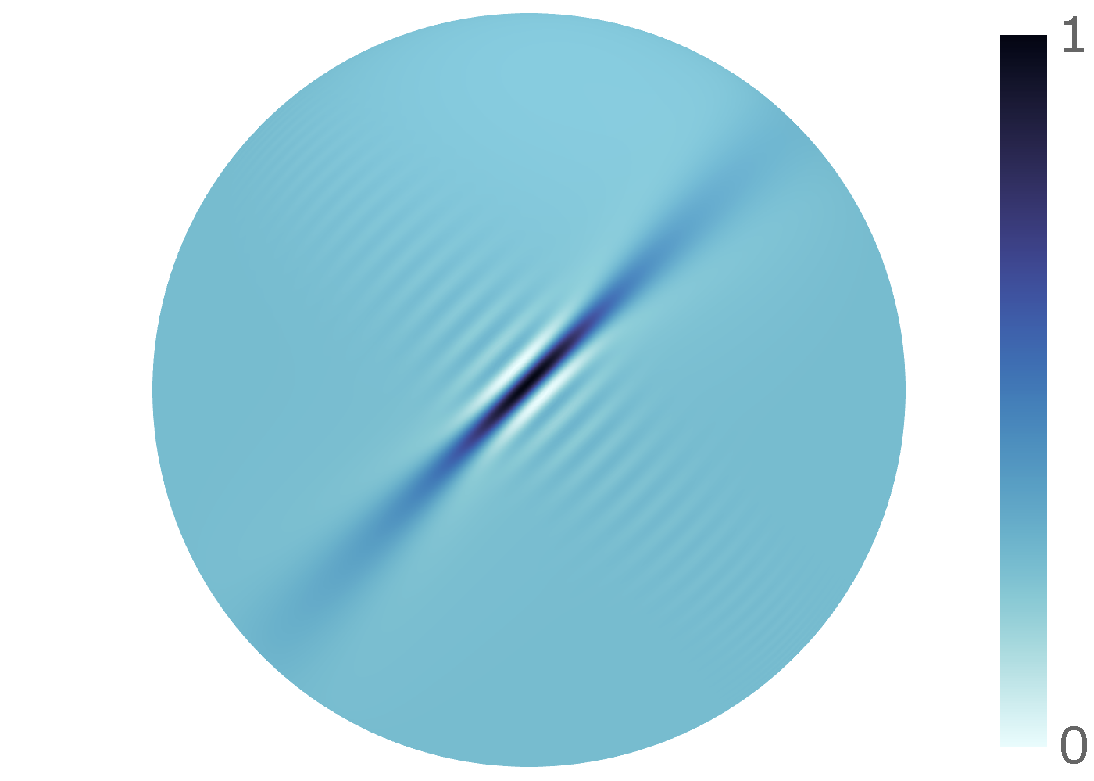
\includegraphics[trim={4 7 3 6},clip,width=.5\textwidth]{harmonic_gaussian_100lsig_10msig_L128_res512_real_norm.pdf}}
	\hfill
	\subfloat[\(\Re\big\{\pixel{f_{B}}\big\}\)]  % chktex 21
	{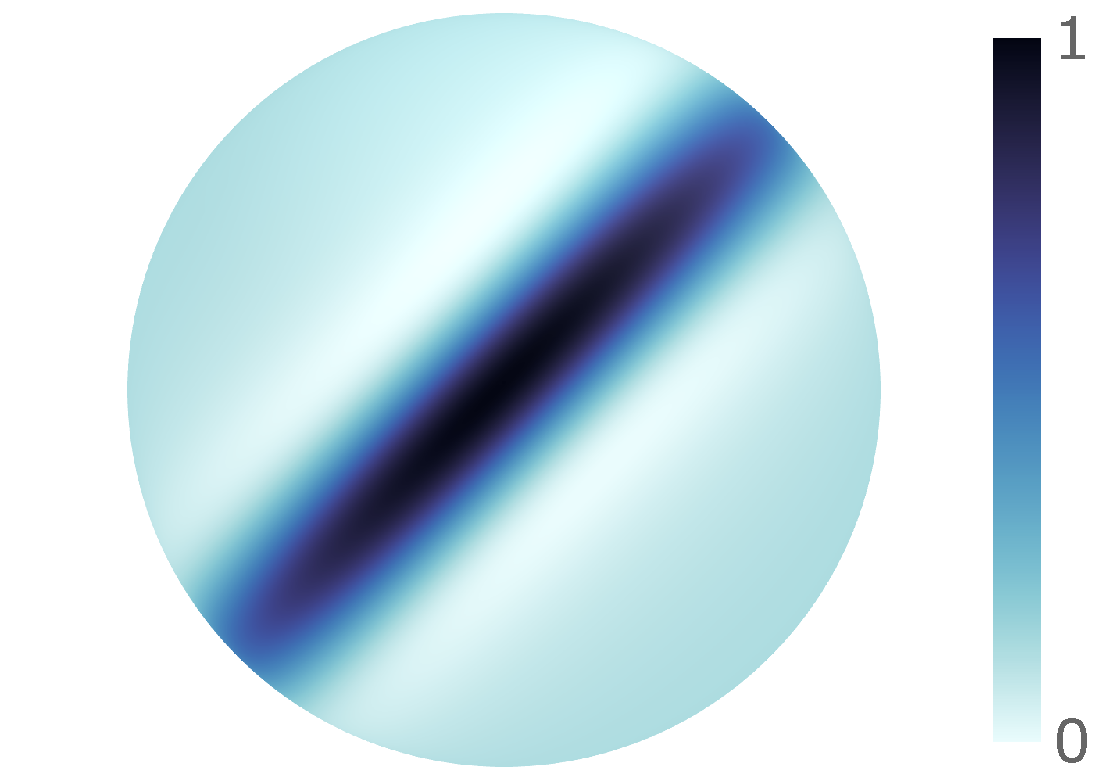
\includegraphics[trim={4 7 3 6},clip,width=.5\textwidth]{harmonic_gaussian_10lsig_10msig_L128_res512_real_norm.pdf}}
	\newline
	\subfloat[\(\Re\big\{\pixel{(\translation{\omega'}f_{A})}\big\}\)]  % chktex 21
	{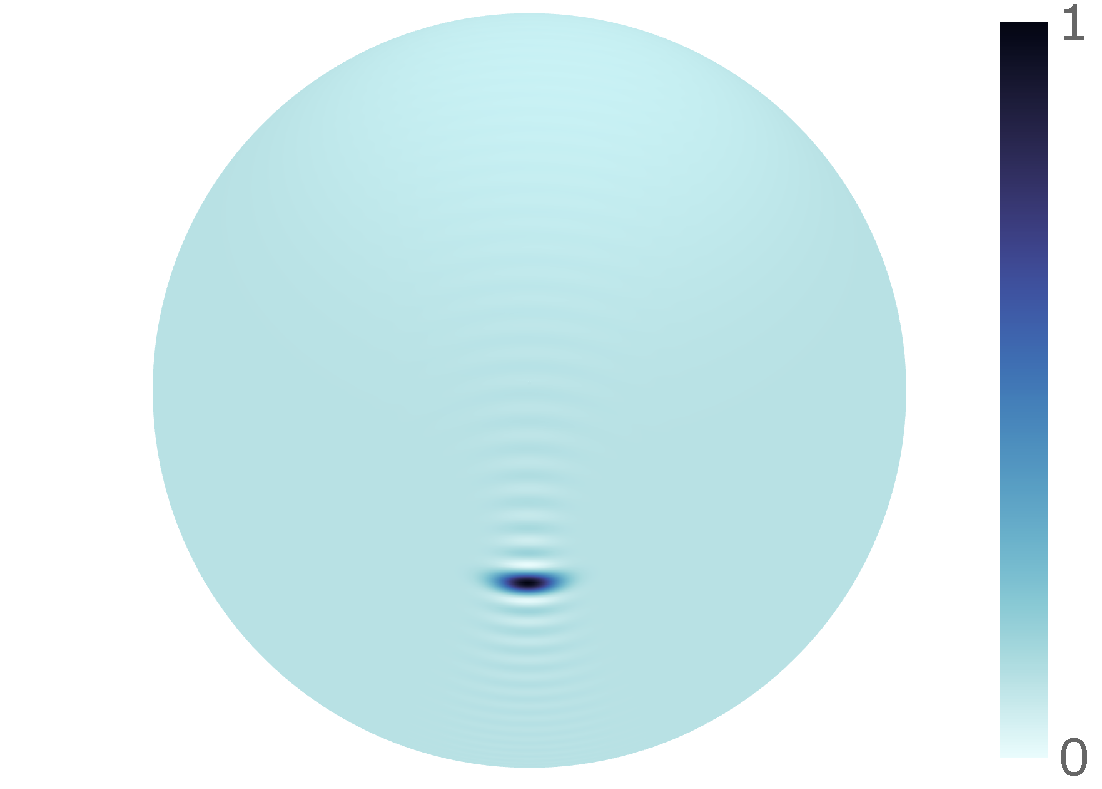
\includegraphics[trim={4 7 3 6},clip,width=.5\textwidth]{harmonic_gaussian_100lsig_10msig_L128_translate_alpha3pi4_beta1pi8_res512_real_norm.pdf}}
	\hfill
	\subfloat[\(\Re\big\{\pixel{(\translation{\omega'}f_{B})}\big\}\)]  % chktex 21
	{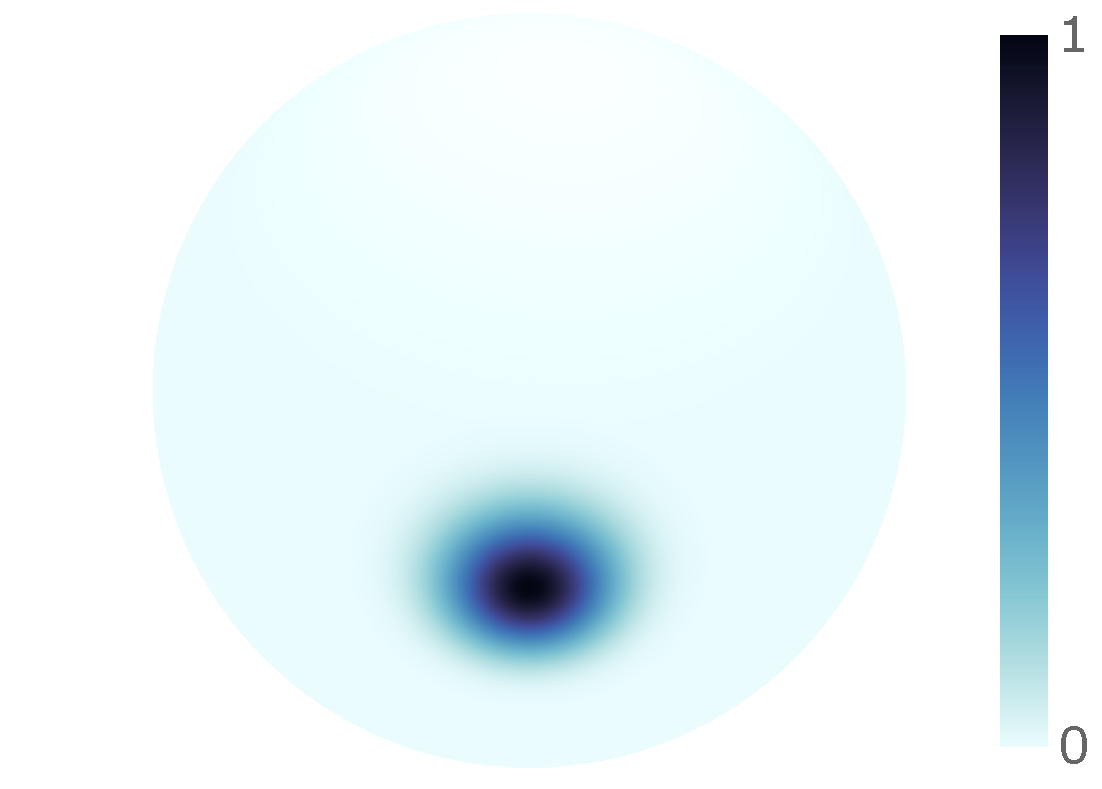
\includegraphics[trim={4 7 3 6},clip,width=.5\textwidth]{harmonic_gaussian_10lsig_10msig_L128_translate_alpha3pi4_beta1pi8_res512_real_norm.pdf}}
	\caption[
		Two harmonic Gaussians on the north pole and then translated
	]{
		The top row presents a harmonic Gaussian on the north pole (bandlimited at \(L=128\)) for two different \((\sigma_{\ell},\sigma_{m})\) values, \cf{} \cref{eq:chapter3_harmonic_gaussian}.
		Panel (a) corresponds to a more elongated kernel \(f_{A}\), where \((\sigma_{\ell},\sigma_{m}) = (10^{2},10^{1})\).
		The harmonic Gaussian is translated to some \(\omega'=(\theta',\phi')\) as shown in panel (c).
		Whereas panel (b) corresponds to a more symmetric kernel \(f_{B}\), where \((\sigma_{\ell},\sigma_{m}) = (10^{1},10^{1})\), with the corresponding translated function in panel (d).
		The colour is between zero and one, reflecting the scaled intensity of the field.
	}\label{fig:chapter3_harmonic_gaussian}
\end{figure}


\subsection{Convolution}\label{sec:chapter3_convolution}

To study the effect of the sifting convolution, consider the Earth Gravitational Model EGM2008 dataset~\cite{Pavlis2013}.
This dataset is the topographic map of the Earth.
\cref{fig:chapter3_earth} presents the dataset up to an order of \(L=128\).
The sifting convolution is then performed between the Earth representation and the harmonic Gaussian with the resultant plot given in \cref{fig:chapter3_convolved}.
As expected, when the elongated kernel is considered, as shown in the left panel, the result exhibits greater anisotropic smoothing than when considering the symmetric kernel, as shown in the right panel.
It is clear that the sifting convolution supports directional kernels to perform anisotropic filtering (smoothing), while the output remains on the sphere.

\begin{figure}[htpb]
	\centering\capstart{}
	\includegraphics[trim={23 7 3 6},clip,width=.5\textwidth]{earth_L128_res512_real_norm.pdf}
	\caption[
		The EGM2008 dataset
	]{
		EGM2008 dataset centred on a view of South America (bandlimited at \(L=128\)).
		The colour is between zero and one, reflecting the scaled intensity of the field.
	}\label{fig:chapter3_earth}
\end{figure}


\begin{figure}[htpb]
	\centering\capstart{}
	\subfloat[\(\Re{\pixel{\convolution{f_{A}}{g}}}\)]{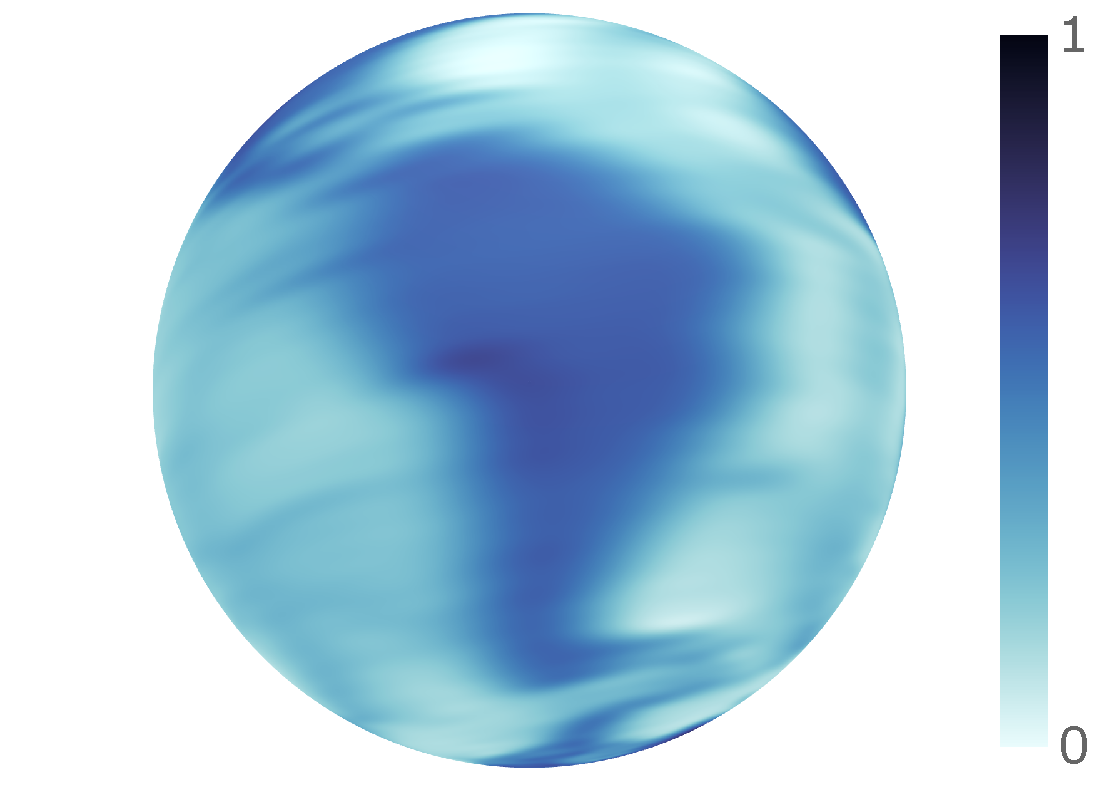
\includegraphics[trim={23 7 3 6},clip,width=.5\textwidth]{harmonic_gaussian_100lsig_10msig_L128_convolved_earth_L128_res512_real_norm.pdf}}
	\hfill
	\subfloat[\(\Re{\pixel{\convolution{f_{B}}{g}}}\)]{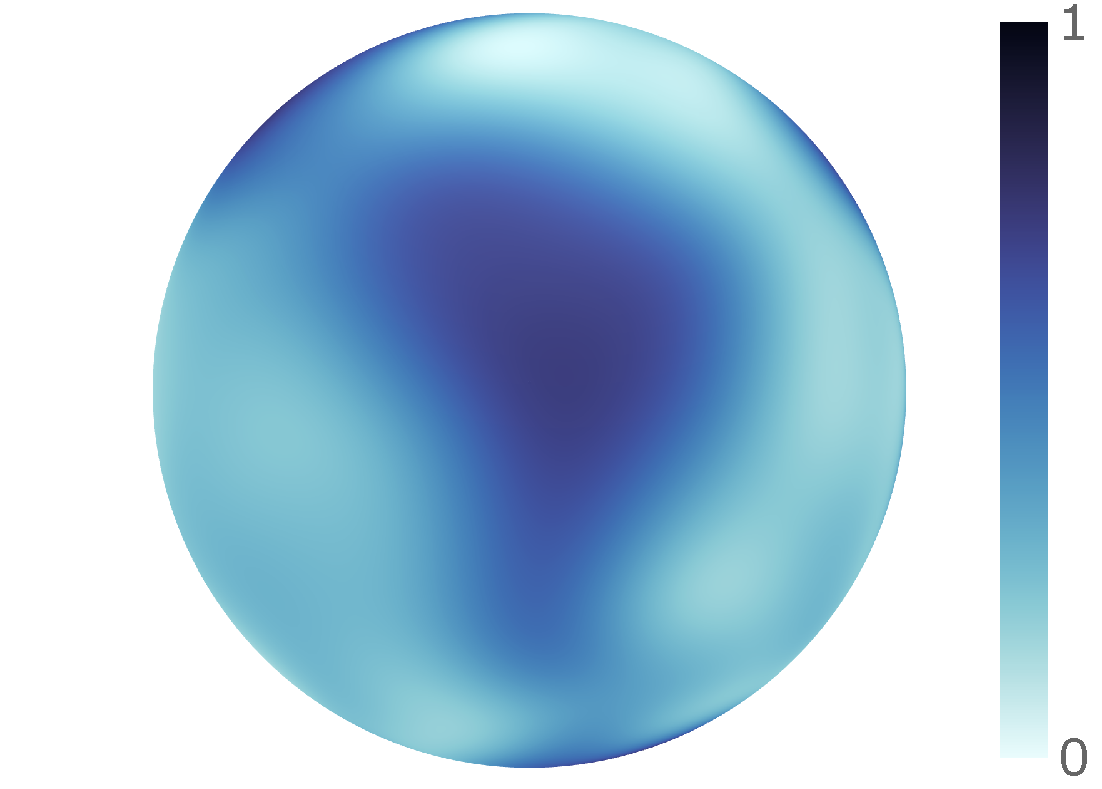
\includegraphics[trim={23 7 3 6},clip,width=.5\textwidth]{harmonic_gaussian_10lsig_10msig_L128_convolved_earth_L128_res512_real_norm.pdf}}
	\caption[
		Two harmonic Gaussians convolved with a map of the Earth
	]{
		The real part of the sifting convolution between the EGM2008 dataset and the harmonic Gaussian, rotated to view of South America (bandlimited at \(L=128\)).
		Panel (a) corresponds to a more elongated kernel \(f_{A}\), where \((\sigma_{\ell},\sigma_{m}) = (10^{2}, 10^{1})\); whereas panel (b) corresponds to a more symmetric kernel \(f_{B}\), where \((\sigma_{\ell},\sigma_{m}) = (10^{1}, 10^{1})\).
		As expected, the resultant sifting convolved Earth map exhibits greater anisotropic smoothing in panel (a) than in panel (b).
		It is clear that the sifting convolution supports directional kernels to perform anisotropic filtering (smoothing), while the output remains on the sphere.
		The colour is between zero and one, reflecting the scaled intensity of the field.
	}\label{fig:chapter3_convolved}
\end{figure}


\section{Conclusion}\label{sec:chapter3_conclusion}

This chapter presents the sifting convolution on the sphere and demonstrates its application.
The convolution accepts directional functions as inputs, has an output which remains on the sphere, and is efficient to compute.
The sifting convolution is defined in the usual manner through the inner product but with an alternative translation operator on the sphere.
This follows by analogy with the Euclidean translation when viewed as a convolution with a shifted Dirac delta function.
An illustration of the sifting convolution on the topographic map of the Earth demonstrates that it supports directional kernels to perform anisotropic filtering, while its output remains on the sphere.
Convolutions are an important part of signal processing techniques, hence, the sifting convolution can play an integral role in constructions of alternate spherical analysis techniques, which is the focus of \cref{sec:chapter4}.

\chapter{Slepian Scale-Discretised Wavelets on Manifolds}\label{sec:chapter4}

\section{Introduction}

Many fields measure data which are intrinsically non-Euclidean in structure and are better modelled by manifolds or graphs.
One manifold, in particular, which is in commonplace in science and engineering is the sphere, such as in cosmology~\cite{Bennett1996}, geophysics~\cite{Simons2006}, planetary science~\cite{Turcotte1981}, computer graphics~\cite{Ramamoorthi2004}, and signal processing~\cite{Roddy2021a}.
Often data are not observed/are missing in some region of the manifold, and hence methods which work over the whole manifold may not be appropriate.
One such example, in the spherical setting, is in cosmic microwave background analyses where foreground microwave emissions dominate the region around the  Galactic plane and are often removed~\cite{Mortlock2002}.
Wavelets are a typical approach to deal with problems of this form, which allow the probing of spatially localised, scale-dependent features of the signal.
Contamination of the wavelet coefficients at the boundaries of the region, however, still presents a problem.
Hence, to overcome this, Slepian wavelets are constructed within the region itself.

\section{Mathematical Background and Problem Formulation}

\subsection{Mathematical Preliminaries}

\subsubsection{Riemannian Manifolds}

Let \(\manifold{}\) denote a compact, smooth, connected \(d\)-dimensional Riemannian manifold without boundary contained in \(\mathbb{R}^{n}\).
The Hilbert space \(\hilbert{\manifold}\) is formed by the set of functions \(f : \manifold \to \mathbb{R}\) that are square-integrable with respect to the Riemannian volume \(\meshVolume{}\).
The geodesic distance between two points is denoted \(r(x,y)\), and the Laplace-Beltrami operator on \(\manifold{}\) is denoted \(\laplacian{}\).
Let the set of all isometries between two manifolds \(\manifold{}\) and \(\manifold'\) be denoted \(\isom{\manifold,\manifold'}\), and set \(\isom{\manifold} = \isom{\manifold,\manifold}\) to be the isometry group of \(\manifold{}\).
Similarly, \(\diff{\manifold} = \diff{\manifold,\manifold}\) is set to be the diffeomorphism group on \(\manifold{}\).

In practice, one must discretise the manifolds and represent them as graphs.
A review of graphs is presented in \cref{sec:chapter4_graphs}.

\subsubsection{Graphs}\label{sec:chapter4_graphs}

\subsubsection{Polygonal Meshes}

\begin{figure}[htp]
	\centering
	\subfloat[\(\mesh{\phi_{3}}\)]
	{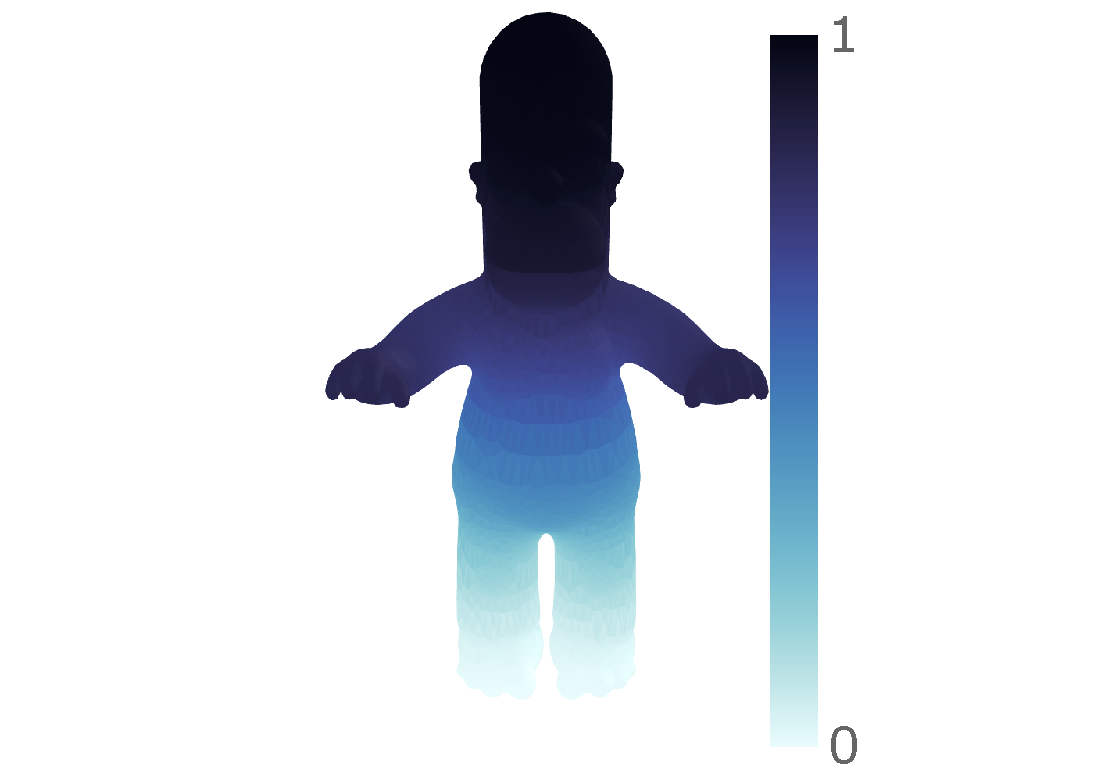
\includegraphics[trim={156 8 21 6},clip,width=.25\textwidth]{homer_rank2_lam1-325328e-03_norm.pdf}} % chktex 8
	\hfill
	\subfloat[\(\mesh{\phi_{4}}\)]
	{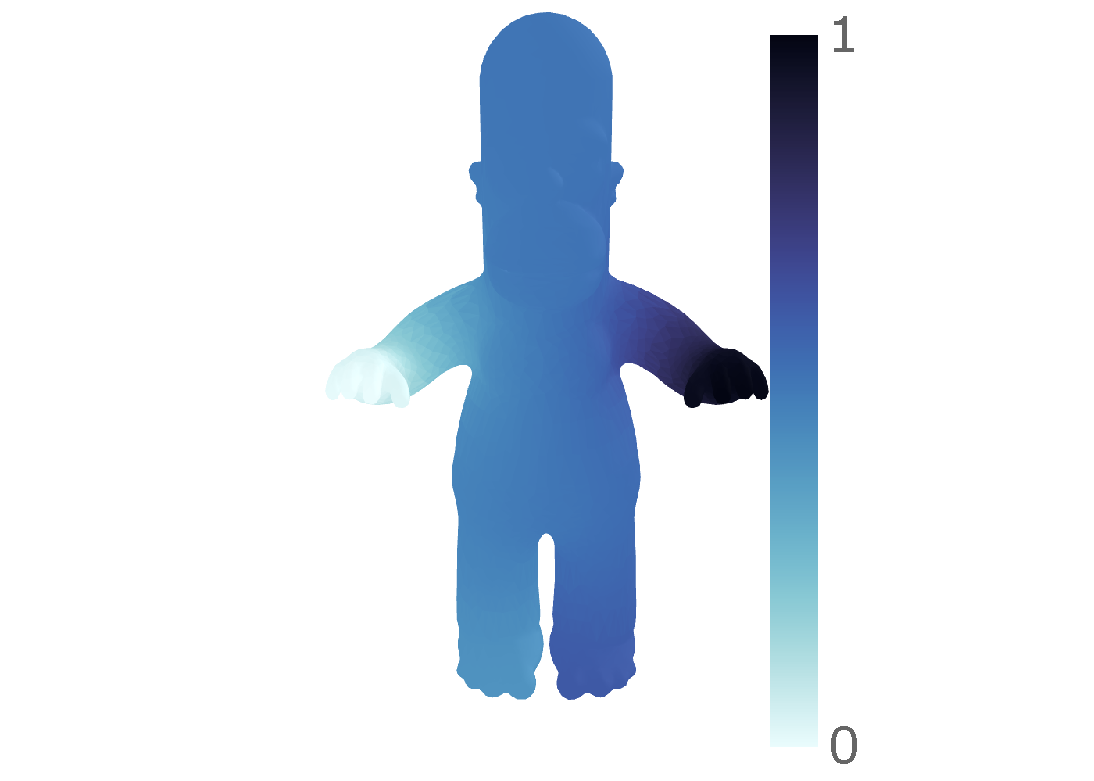
\includegraphics[trim={156 8 21 6},clip,width=.25\textwidth]{homer_rank3_lam2-425344e-03_norm.pdf}} % chktex 8
	\hfill
	\subfloat[\(\mesh{\phi_{5}}\)]
	{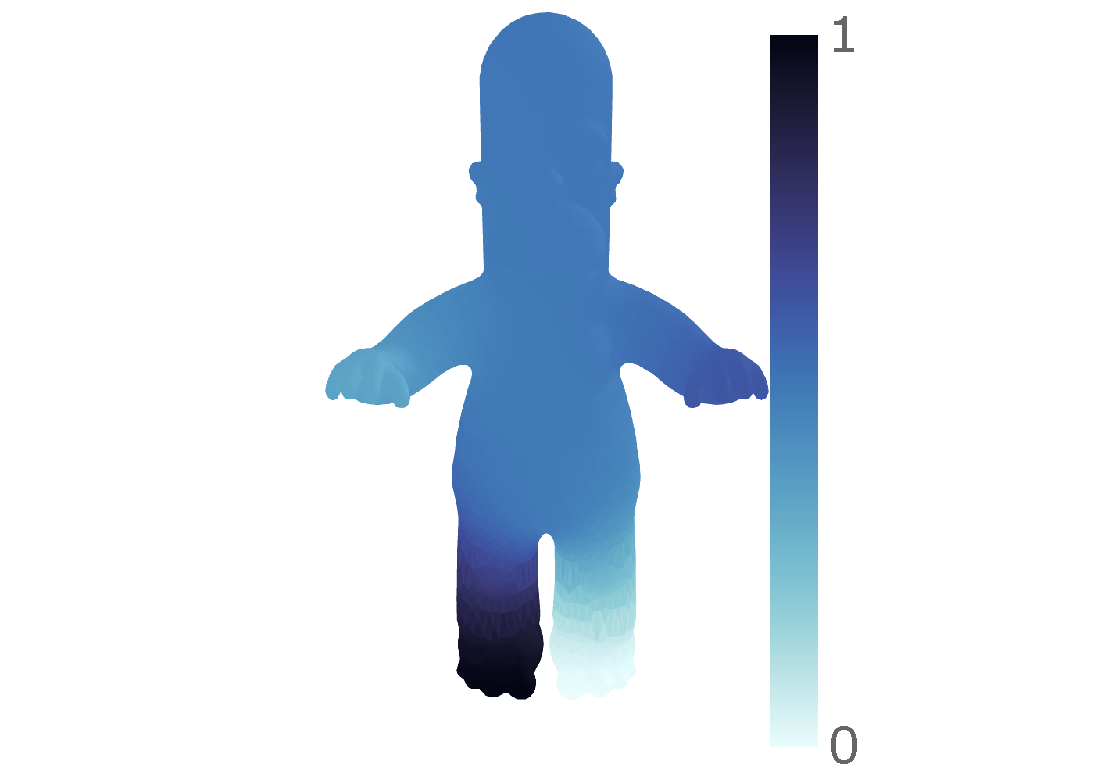
\includegraphics[trim={156 8 21 6},clip,width=.25\textwidth]{homer_rank4_lam2-706937e-03_norm.pdf}} % chktex 8
	\hfill
	\subfloat[\(\mesh{\phi_{6}}\)]
	{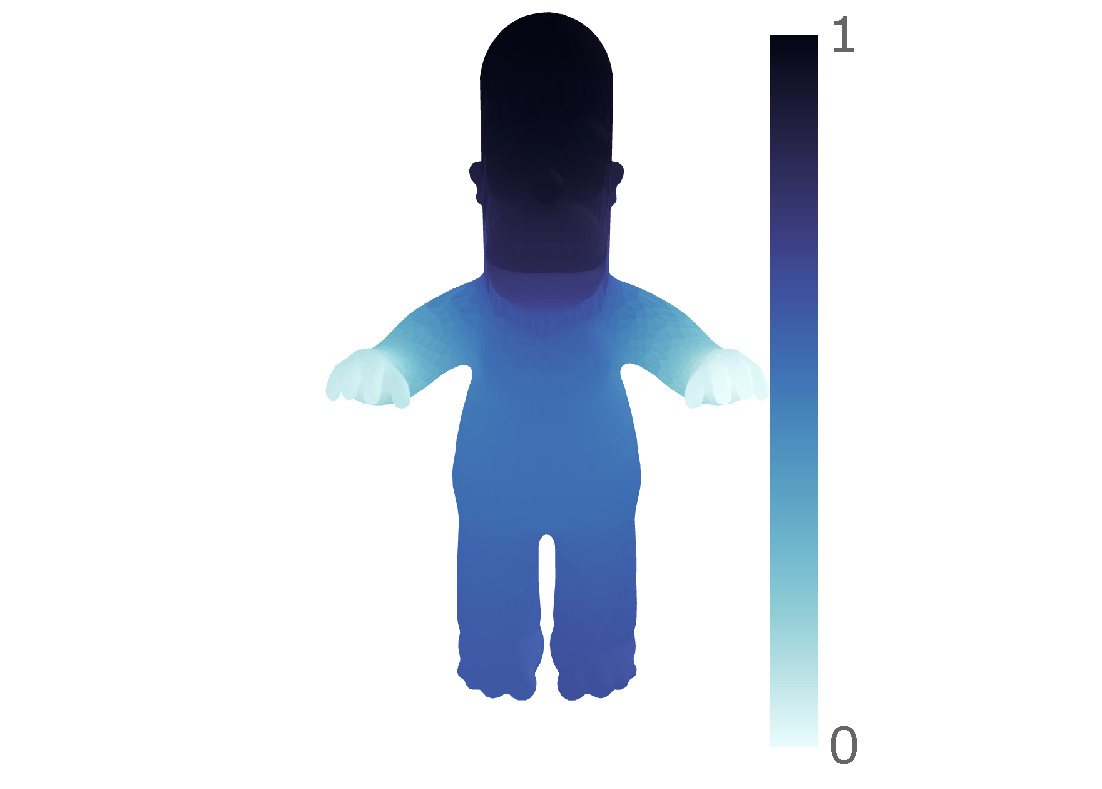
\includegraphics[trim={156 8 21 6},clip,width=.25\textwidth]{homer_rank5_lam2-851096e-03_norm.pdf}} % chktex 8
	\newline
	\subfloat[\(\mesh{\phi_{7}}\)]
	{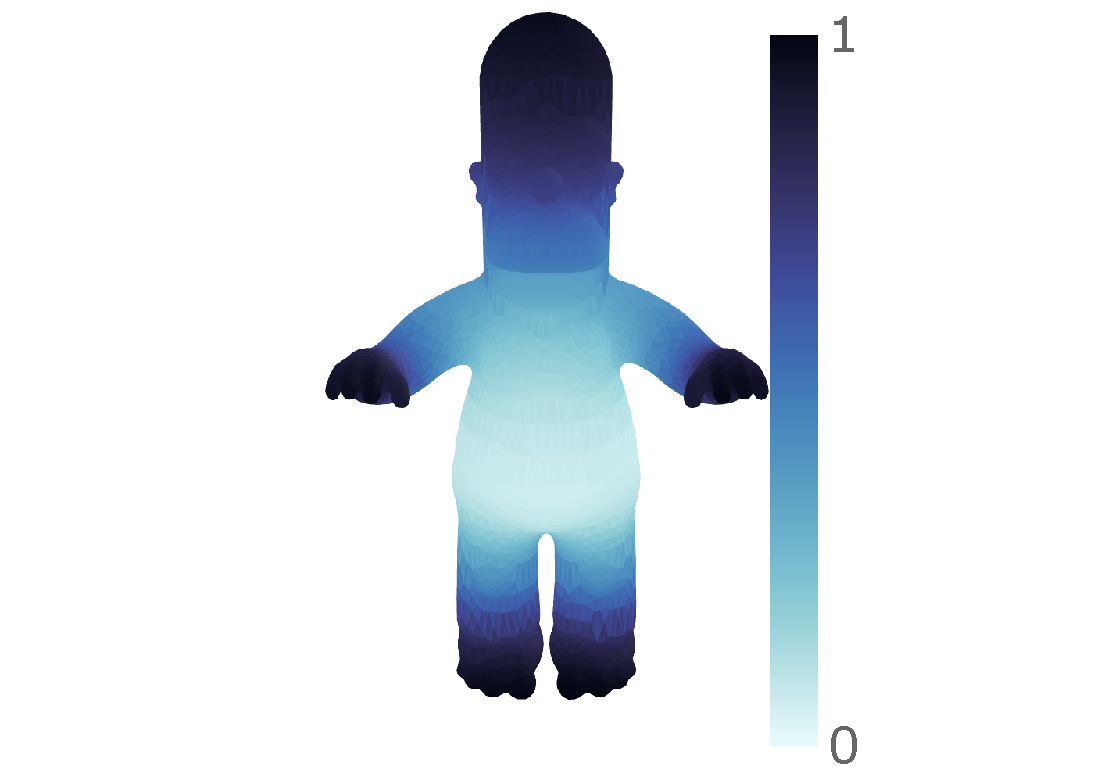
\includegraphics[trim={156 8 21 6},clip,width=.25\textwidth]{homer_rank6_lam7-806422e-03_norm.pdf}} % chktex 8
	\hfill
	\subfloat[\(\mesh{\phi_{8}}\)]
	{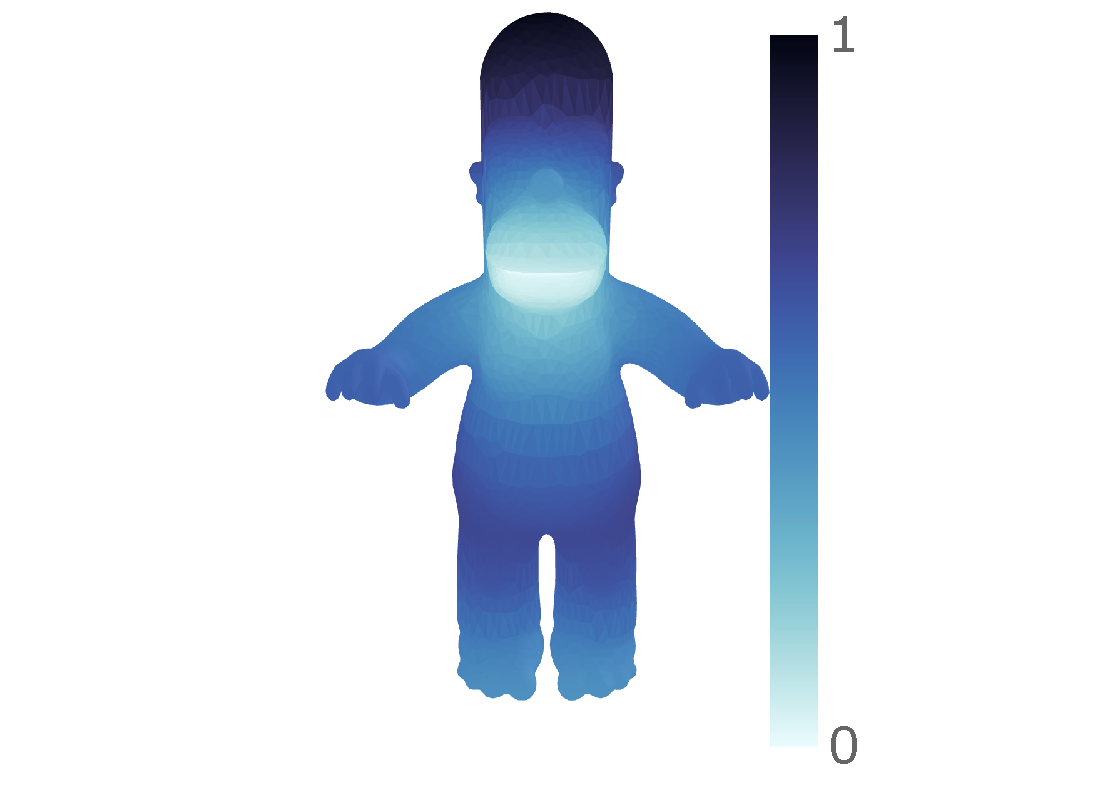
\includegraphics[trim={156 8 21 6},clip,width=.25\textwidth]{homer_rank7_lam1-164387e-02_norm.pdf}} % chktex 8
	\subfloat[\(\mesh{\phi_{9}}\)]
	{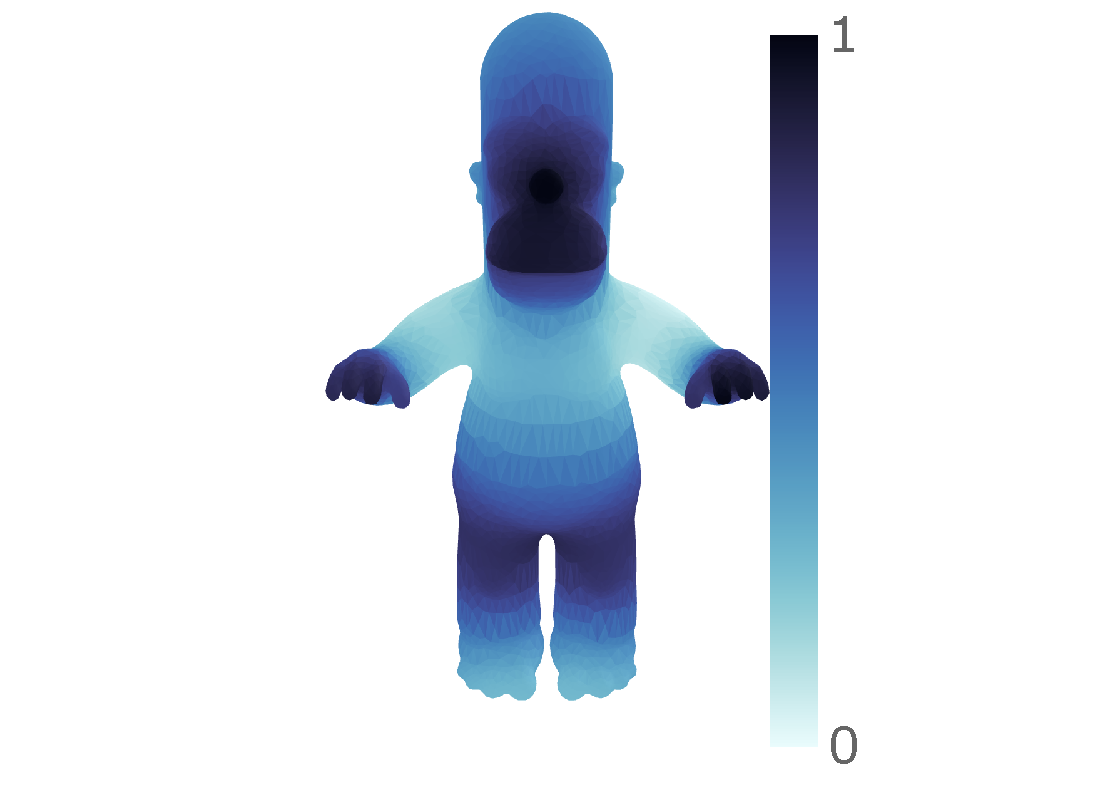
\includegraphics[trim={156 8 21 6},clip,width=.25\textwidth]{homer_rank8_lam1-738974e-02_norm.pdf}} % chktex 8
	\hfill
	\subfloat[\(\mesh{\phi_{10}}\)]
	{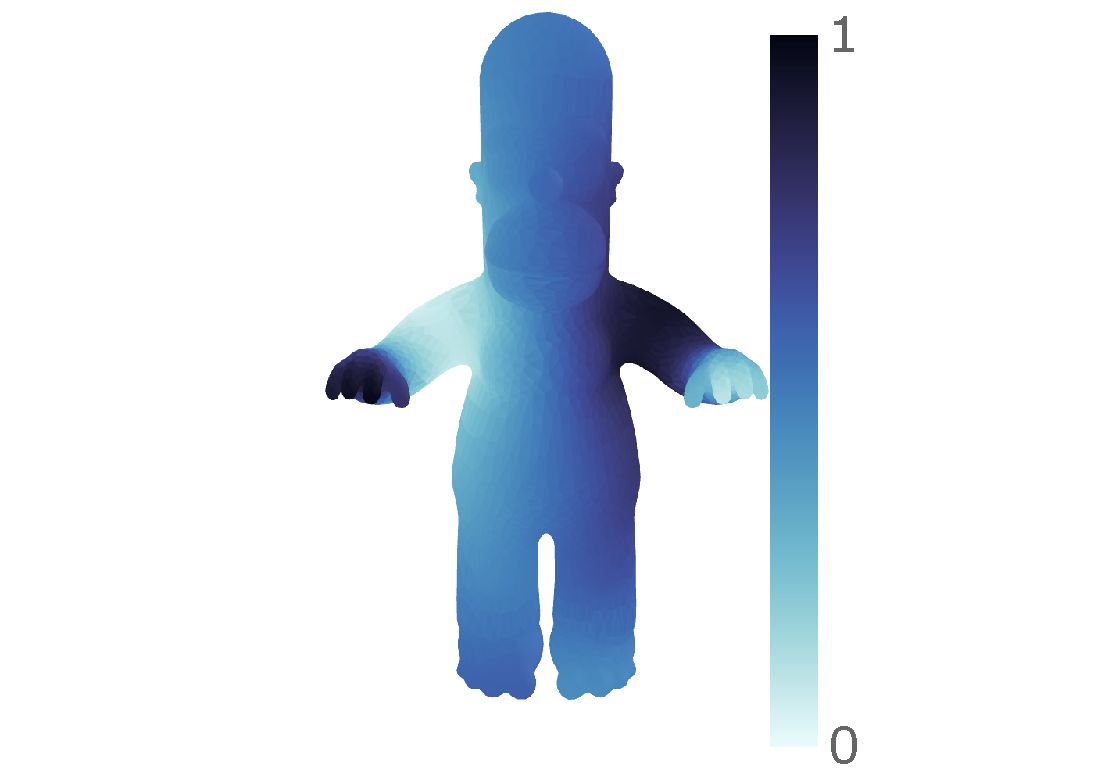
\includegraphics[trim={156 8 21 6},clip,width=.25\textwidth]{homer_rank9_lam1-827015e-02_norm.pdf}} % chktex 8
	\caption{
		The third to tenth eigenvectors of the mesh Laplacian of a Homer Simpson mesh ordered by increasing eigenvalue (frequency).
		In total \(\num{1275}\) basis functions of the \(\num{5103}\) vertex mesh were computed.
		Whilst the eigenvectors are defined on the vertices, the values have been averaged onto the faces for the plot.
	}\label{fig:chapter4_eigenhomers}
\end{figure}


\subsection{Problem Formulation}\label{sec:chapter4_problem_formulation}

This work generalises Slepian scale-discretised wavelets on the sphere~\cite{Roddy2021a} to arbitrary manifolds.
Here, the basis functions of the Slepian concentration problem are built from the eigenvectors of the Laplace-Beltrami operator of the manifold, as opposed to the spherical harmonics.
In the aforesaid work, the wavelets are constructed through a tiling of the Slepian line (akin to the harmonic line) in an analogous manner to~\cite{Wiaux2008,McEwen2018}.
The sifting convolution~\cite{Roddy2021} allows one to perform convolutions where both inputs are directional, whilst the output remains on the sphere.
By leveraging this convolution, the wavelet transforms in the Slepian domain are built on a region of the sphere (\cf{} manifold) to ensure exact reconstruction.
Convolutions are typically not well-defined on manifolds.
The sifting convolution, however, is a product in harmonic space and as such can be applied effectively to manifolds.

In \cref{sec:chapter4_working_with_manifolds}, the Slepian spatial-spectral concentration problem is presented in the manifold setting --- in particular, the spatial concentration of a bandlimited function.
The sifting convolution~\cite{Roddy2021} is then defined similarly, allowing for wavelet transforms on the manifold to be constructed.

\section{Working with Manifolds}\label{sec:chapter4_working_with_manifolds}

In this section a review of the Slepian spatial-spectral concentration problem adapted to manifolds is presented in \cref{sec:chapter4_slepian_concentration_problem_manifolds}.
A review of the sifting convolution follows in \cref{sec:chapter4_sifting_convolution_manifolds} which allows one to perform convolutions on manifolds.

\subsection{Slepian Concentration Problem on Manifolds}\label{sec:chapter4_slepian_concentration_problem_manifolds}

The problem of spatial concentration of bandlimited signals (likewise spectral concentration of spacelimited signals) was first studied by Slepian, Landau and Pollak in the 1960s~\cite{Slepian1961,Landau1961,Landau1962}.
Initially for time domain signals, it has since been extended to other domains such as signals on the sphere~\cite{Simons2006,Roddy2021a,Xu1983,Wieczorek2005}.
This work considers optimally concentrated functions within a region \(R\) of a manifold \(\manifold{}\), an example of which is shown in \cref{fig:chapter4_region}.

% Inspired by Fionn Fitzmaurice's differential geometry notes
% https://gist.github.com/fionn/f27ddeadba97f3dabbf97527b05b33e5
\begin{figure}[htp]
	\centering
	\resizebox{0.75\textwidth}{!}{%
		\begin{tikzpicture}
			\begin{scope}
				\draw [postaction={stipple={amplitude=0.5cm}},
					postaction={stipple={amplitude=0.25cm}}]
				(0, 0) .. controls ++(65:-1.5) and ++(95:1) .. (-1.5, -4)
				(-1.5, -4) .. controls ++(195:-1.3) and ++(195:1) .. (3, -4)
				(3, -4) .. controls ++(95:2) and ++(95:-1) .. (4, 0)
				node[below right] {$\mathcal{M}$}
				(4, 0) .. controls ++(195:1) and ++(195:-1) .. (0, 0);
			\end{scope}
			\draw [use Hobby shortcut, % .. syntax
				closed=true, % connects region outline
				pattern=north east lines] % direction of lines
			(0.7,-2.3) .. (1.2,-2.6) .. (2.3,-2.2) .. (2,-1.8) .. (1.2,-1.3) .. (0.7,-1.4) .. (0.8,-1.9);
			\node at (1.8,-1.3) {\(R\)};
		\end{tikzpicture}%
	}
	\caption{
		In various domains, data are observed on a partial region of a manifold \(\mathcal{M}\), such as \(R\).
	}\label{fig:chapter4_region}
\end{figure}


\subsubsection{Spatial Concentration of a Bandlimited Function}

To maximise the spatial energy concentration of a bandlimited signal \(f \in \hilbert{\manifold}\), the following ratio must be maximised:
%
\begin{equation}
	\mu
	%
	= \frac{\integrateRegion{\meshVolume} \abs{\mesh{f}}^{2}}{\integrateManifold{x} \abs{\mesh{f}}^{2}},
\end{equation}
%
where spatial concentration is measured by \(0 < \mu < 1\).
In harmonic space this can be simplified to a sum
%
\begin{equation}\label{eq:chapter4_spatial_concentration_ratio}
	\mu
	%
	= \frac{\sum\limits_{i} f_{i} \sum\limits_{j} D_{i,j} f_{j}}{\meshSum \abs{f_{i}}^{2}},
\end{equation}
%
where
%
\begin{equation}
	D_{i,j}
	%
	= \integrateRegion{\meshVolume \mesh{\phi_{i}} \mesh{\phi_{j}}}
\end{equation}
%
is a square matrix including all basis functions of the manifold.
Rewriting \cref{eq:chapter4_spatial_concentration_ratio} as a matrix variational problem
%
\begin{equation}
	\mu
	%
	= \frac{\transpose{\vb{f}} \vb{D} \vb{f}}{\transpose{\vb{f}} \vb{f}},
\end{equation}
%
where \(\vb{f}\) are the harmonic coefficients of \(\mesh{f}\), and are the solutions to the eigenproblem
%
\begin{equation}\label{eq:chapter4_eigenproblem}
	\vb{D}\vb{f}
	%
	= \mu \vb{f}.
\end{equation}
%
The eigenvalues \(\mu_{i}\) act as a measure of the relative spatial concentration
%
\begin{equation}
	1 > \mu_{1} \geq \mu_{2} \geq \ldots \geq \mu_{\imax} > 0, % chktex 11
\end{equation}
%
of the corresponding eigenvectors
%
\begin{equation}
	\vb{f}_{1},\ \vb{f}_{2},\ \ldots,\ \vb{f}_{\imax}.
\end{equation}
%
No bandlimited function can be restricted exactly within a region \(R\) and hence \(\mu_{1}<1\).
Due to the positive definiteness of \(\vb{D}\) the smallest eigenvalue \(\mu_{\imax}\) is strictly greater than zero.
A manifold analogue of the \emph{Shannon number} can be constructed by
%
\begin{equation}\label{eq:chapter4_shannon}
	N
	%
	= \frac{A_{R}}{A_{\manifold}} \imax,
\end{equation}
%
where \(A\) denotes the area of the region \(R\)/manifold \(\manifold{}\).
The Shannon number is a good estimate of the number of significant eigenvalues~\cite{Percival1993}.

\subsubsection{Slepian Decomposition}

The Slepian functions provide an alternative orthogonal basis of the manifold, decomposing a function \(f \in \hilbert{\manifold}\) into this basis
%
\begin{equation}
	\mesh{f}
	%
	= \sum\limits_{p=1}^{\imax} \slepian{f} \mesh{\slepian{S}},
\end{equation}
%
where the sum is over all basis functions of the manifold.
For a well-localised function in the region \(R\) (\ie{} \(f \in \hilbert{R}\)) the sum may be truncated at the Shannon number
%
\begin{equation}
	\mesh{f}
	%
	\approx \sum\limits_{p=1}^{N} \slepian{f} \mesh{\slepian{S}}
	%
	= \slepianSum \slepian{f} \mesh{\slepian{S}},
\end{equation}
%
where the last line introduces a shorthand notation.
The Slepian coefficients \(\slepian{f}\) are calculated through the usual projection on to the basis functions
%
\begin{equation}
	\slepian{f}
	%
	= \braket{f}{\slepian{S}}.
\end{equation}

The Slepian coefficients of a well-localised function may be computed with an integral over the region \(R\) rather than an integral over the whole manifold \(\manifold{}\):
%
\begin{equation}
	\slepian{f}
	%
	= \frac{1}{\slepian{\mu}} \integrateRegion{\meshVolume} \mesh{f} \mesh{\slepian{S}},
\end{equation}
%
as
%
\begin{align}
	\integrateRegion{\meshVolume} \mesh{f} \mesh{\slepian{S}}
	%
	 & = \slepianSum['] \slepian[']{f} \integrateRegion{\meshVolume} \mesh{\slepian[']{S}} \mesh{\slepian{S}} \nonumber \\
	%
	 & = \slepianSum['] \slepian[']{f} \transpose{\slepian{\vb{S}}} \vb{D} \slepian[']{\vb{S}} \nonumber                \\
	%
	 & = \slepian{f} \slepian{\mu},
\end{align}
%
where \(\vb{S}\) are the harmonic coefficients of \(\mesh{\slepian{S}}\).
Note the use of the orthogonality results
%
\begin{equation}\label{eq:chapter4_orthogonality_manifold}
	\integrateManifold{x} \mesh{\slepian{S}} \mesh{\slepian[']{S}}
	%
	= \transpose{\slepian[']{\vb{S}}} \slepian{\vb{S}}
	%
	= \delta_{pp'},
\end{equation}
%
and
%
\begin{equation}
	\integrateRegion{\meshVolume} \mesh{\slepian{S}} \mesh{\slepian[']{S}}
	%
	= \transpose{\slepian[']{\vb{S}}} \vb{D} \slepian{\vb{S}}
	%
	= \slepian{\mu} \transpose{\slepian[']{\vb{S}}} \slepian{\vb{S}}
	%
	= \slepian{\mu} \delta_{pp'}.
\end{equation}

To transform from Slepian coefficients to the basis functions of the manifold
%
\begin{equation}\label{eq:chapter4_slepian_to_harmonic}
	f_{i}
	%
	= \integrateManifold{x} \mesh{f} \mesh{\phi_{i}}
	%
	= \slepianSum \slepian{f} {(\slepian{S})}_{i},
\end{equation}
%
where \({(\slepian{S})}_{i}\) are the eigenvectors of the eigenproblem \cref{eq:chapter4_eigenproblem}:
%
\begin{equation}
	{(\slepian{S})}_{i}
	%
	= \integrateManifold{x} \mesh{\slepian{S}} \mesh{\phi_{i}}.
\end{equation}
%
The inverse operation of \cref{eq:chapter4_slepian_to_harmonic} is
%
\begin{equation}\label{eq:chapter4_harmonic_to_slepian}
	\slepian{f}
	%
	= \integrateManifold{x} \mesh{f} \mesh{\slepian{S}}
	%
	= \sum\limits_{i} f_{i} {(\slepian{S})}_{i}.
\end{equation}

\subsection{Sifting Convolution on Manifolds}\label{sec:chapter4_sifting_convolution_manifolds}

A central part of wavelet transforms is the convolution.
On \(\mathbb{R}^{d}\), the convolution of a signal \(f \in \hilbert{\mathbb{R}^{d}}\) with a filter \(g \in \hilbert{\mathbb{R}^{d}}\) is defined by translating \(g\) against \(f\); however, general manifolds do not have well-defined translations.
Recently developed by the authors of this work, the sifting convolution~\cite{Roddy2021} is built on a translation which simply involves a product of the basis functions.
Initially defined in the spherical setting, the sifting convolution can be arbitrarily extended to other domains.

The translation operator on the manifold is
%
\begin{equation}
	\mesh{(\translation{y}\phi_{i})}
	%
	\equiv \meshY{\phi_{i}} \mesh{\phi_{i}},
\end{equation}
%
where \(y\) is a point on the manifold.
An arbitrary function \(f \in \hilbert{\manifold}\) is translated thus
%
\begin{equation}
	\mesh{(\translation{y}f)}
	%
	= \sum\limits_{i} f_{i} \meshY{\phi_{i}} \mesh{\phi_{i}},
\end{equation}
%
implying
%
\begin{equation}
	{(\translation{y}f)}_{i}
	%
	= f_{i} \meshY{\phi_{i}}.
\end{equation}
%
The sifting convolution on the manifold of \(f,\ g \in \hilbert{\manifold}\) follows by the inner product
%
\begin{equation}
	\mesh{\convolution{f}{g}}
	%
	\equiv \integrateManifold{y} \meshY{(\translation{x}f)} \meshY{g},
\end{equation}
%
which is a product in harmonic space
%
\begin{equation}
	{\convolution{f}{g}}_{i}
	%
	= f_{i} g_{i}.
\end{equation}
%
This convolution can be used to define wavelets restricted to a region of the manifold using the basis functions introduced in \cref{sec:chapter4_slepian_concentration_problem_manifolds} in the translation.

\section{Slepian Wavelets}

Here, the Slepian wavelet theory is developed.
Initially, \cref{sec:chapter4_slepian_sifting_convolution} extends the sifting convolution~\cite{Roddy2021} to the Slepian domain.
With a convolution to hand, the Slepian wavelet transform is developed in \cref{sec:chapter4_slepian_scale_discretised_wavelets} --- where an appropriate admissibility condition must hold for exact reconstruction.
The generating functions that define the wavelets are presented in \cref{sec:chapter4_generating_functions}.
Lastly, some properties of the wavelets are discussed in \cref{sec:chapter4_properties}.

\subsection{Slepian Sifting Convolution}\label{sec:chapter4_slepian_sifting_convolution}

To construct wavelets in a region of the manifold a suitable convolution is required.
The sifting convolution on the manifold defined in \cref{sec:chapter4_slepian_concentration_problem_manifolds} and developed by the authors of the current article~\cite{Roddy2021}, can be extended to work with the Slepian functions as a basis.

Consider the sifting convolution of a region on a manifold with the Slepian functions as a localised basis.
The translation is defined as such
%
\begin{equation}
	\mesh{(\translation{y}\slepian{S})}
	%
	\equiv \meshY{\slepian{S}} \mesh{\slepian{S}},
\end{equation}
%
where \(y\) is a point on the manifold and \(\mesh{\slepian{S}}\) are the Slepian functions defined in \cref{sec:chapter4_slepian_concentration_problem_manifolds}.
Hence, the translation of an arbitrary function \(f \in \hilbert{R}\) is
%
\begin{equation}
	\mesh{(\translation{y}f)}
	%
	= \slepianSum \slepian{f} \meshY{\slepian{S}} \mesh{\slepian{S}},
\end{equation}
%
which is the following in Slepian space
%
\begin{equation}
	\slepian{(\translation{y}f)}
	%
	= \slepian{f} \mesh{\slepian{S}}.
\end{equation}
%
As before, the sifting convolution between two functions \(f,\ g \in \hilbert{R}\) is
%
\begin{equation}
	\mesh{\convolution{f}{g}}
	%
	\equiv \integrateManifold{y} \meshY{(\translation{x}f)} \meshY{g},
\end{equation}
%
which becomes a product in Slepian space
%
\begin{equation}
	\slepian{\convolution{f}{g}}
	%
	= \slepian{f} \slepian{g},
\end{equation}
%
and hence is efficient to compute.
Slepian wavelets may now be defined utilising this convolution in Slepian space.

\subsection{Slepian Scale-Discretised Wavelets}\label{sec:chapter4_slepian_scale_discretised_wavelets}

A Slepian wavelet transform can be constructed through a tiling of Slepian space, where \(p\) is restricted to \(N=\imax A_{R}/A_{\manifold}\) (or \(\imax{}\) for whole manifold).
Spatially localised, scale-dependent content of a signal may be probed through a scale-discretised wavelet transform.
The construction of these wavelets is in an analogous manner to~\cite{Wiaux2008,McEwen2018} but are computed in the Slepian basis rather than the basis functions of the sphere (\cf{} manifold).

For a signal of interest \(f \in \hilbert{R}\) concentrated within a region \(R\), the wavelet coefficients \(W^{\Psi^{j}} \in \hilbert{R}\) are defined through a sifting convolution of \(f\) with the wavelet \(\Psi^{j} \in \hilbert{R}\) for wavelet scale \(j\):
%
\begin{align}
	\mesh{W^{\Psi^{j}}}
	%
	 & = \mesh{\convolution{\Psi^{j}}{f}} \nonumber                         \\
	%
	 & = \integrateManifold{y} \meshY{(\translation{x}\Psi^{j})} \meshY{f}.
\end{align}
%
In Slepian space this becomes
%
\begin{equation}\label{eq:chapter4_slepian_wavelet_p}
	\slepian{W}^{\Psi^{j}}
	%
	= \slepian{\Psi}^{j} \slepian{f},
\end{equation}
%
where \(\slepian{\Psi}^{j}\) are the Slepian harmonic coefficients of the wavelet at scale \(j\).

Wavelets are typically paired with a scaling function, each capturing different underlying scales of the signal.
Scaling coefficients \(W^{\Phi} \in \hilbert{R}\) may be similarly defined by a sifting convolution between \(f\) and the scaling function \(\Phi \in \hilbert{R}\):
%
\begin{align}
	\mesh{W^{\Phi}}
	%
	 & = \mesh{\convolution{\Phi}{f}} \nonumber                         \\
	%
	 & = \integrateManifold{y} \meshY{(\translation{x}\Phi)} \meshY{f},
\end{align}
%
or in Slepian space
%
\begin{equation}\label{eq:chapter4_slepian_scaling_p}
	\slepian{W}^{\Phi}
	%
	= \slepian{\Phi} \slepian{f},
\end{equation}
%
where \(\slepian{\Phi}\) are the Slepian coefficients of the scaling function.

Supposing that the wavelets and scaling function satisfy an admissibility condition, a function \(f\) may be reconstructed from its wavelet and scaling coefficients by
%
\begin{equation}\label{eq:chapter4_synthesis}
	\mesh{f}
	%
	= \integrateManifold{y} \bigg(
	%
	\meshY{(\translation{x}\Phi)} \meshY{W^{\Phi}}
	%
	+ \waveletSum \meshY{(\translation{x}\Psi^{j})} \meshY{W^{\Psi^{j}}}
	%
	\bigg),
\end{equation}
%
or in Slepian space
%
\begin{equation}
	\slepian{f}
	%
	= \slepian{W}^{\Phi} \slepian{\Phi}
	%
	+ \waveletSum \slepian{W}^{\Psi^{j}} \slepian{\Psi}^{j}.
\end{equation}
%
The parameters \(J_{0}\) and \(J\) represent the lowest and highest scales \(j\) of the wavelet decomposition respectively --- to ensure exact reconstruction these parameters must be set consistently.
The admissibility condition required for synthesis \cref{eq:chapter4_synthesis} to hold is thus
%
\begin{equation}\label{eq:chapter4_admissibility}
	\abs{\slepian{\Phi}}^{2}
	%
	+ \waveletSum \abs{\slepian{\Psi}^{j}}^{2}
	%
	= 1,\ \forall p.
\end{equation}
%
Wavelets and a scaling function that satisfy this admissibility condition may now be defined.

\subsection{Generating Functions}\label{sec:chapter4_generating_functions}

Consider the smooth generating functions defined by~\cite{Wiaux2008} to tile the Slepian line.
Consider the \(C^{\infty}\) Schwartz function with compact support on \(\interval{-1}{1}\):
%
\begin{equation}
	s(t) \equiv
	%
	\begin{cases}
		\exp(1/(t^{2}-1)), & t \in \interval{-1}{1}    \\
		%
		0,                 & t \notin \interval{-1}{1}
	\end{cases}
\end{equation}
%
for \(t \in \mathbb{R}\).
The positive real parameter \(\lambda \in \realPosParam{}\) may then be introduced to map \(s(t)\) to
%
\begin{equation}
	s_{\lambda}(t)
	%
	\equiv s\bigg(\frac{2\lambda}{\lambda-1}(t-\lambda^{-1}) - 1\bigg),
\end{equation}
%
which has compact support in \(\interval{1/\lambda}{1}\).
One can define the smoothly decreasing function \(k_{\lambda}\) by
%
\begin{equation}
	k_{\lambda}(t)
	%
	\equiv \frac{\int_{t}^{1} \dd{t'} s^{2}_{\lambda}(t')/t'}
	%
	{\int_{1/\lambda}^{1} \dd{t'} s^{2}_{\lambda}(t')/t'},
\end{equation}
%
which is unity for \(t < 1/\lambda{}\), zero for \(t > 1\), and smoothly decreasing from unity to zero for \(t \in \interval{1/\lambda}{1}\).
The wavelet generating function is defined as
%
\begin{equation}
	\kappa_{\lambda}(t)
	%
	\equiv \sqrt{k_{\lambda}(t/\lambda) - k_{\lambda}(t)},
\end{equation}
%
and the scaling function generating function is
%
\begin{equation}
	\eta_{\lambda}(t)
	%
	\equiv \sqrt{k_{\lambda}(t)}.
\end{equation}

An instinctive approach is to define the wavelets \(\slepian{\Psi}^{j}\) from the generating functions \(\kappa_{\lambda}\) to have support on \(\interval{\lambda^{j-1}}{\lambda^{j+1}}\), yielding
%
\begin{equation}
	\slepian{\Psi}^{j}
	%
	\equiv \kappa_{\lambda}\bigg(\frac{p}{\lambda^{j}}\bigg).
\end{equation}
%
For \(p \geq \lambda^{J_{0}}\) the admissibility condition \cref{eq:chapter4_admissibility} is satisfied for these wavelets, where \(J_{0}\) is the lowest wavelet scale used in the decomposition.
Modes that cannot be probed by wavelets can be extracted through the construction of a scaling function \(\Phi{}\) (\ie{} modes with \(p < \lambda^{J_{0}}\)):
%
\begin{equation}
	\slepian{\Phi}
	%
	\equiv \eta_{\lambda}\bigg(\frac{p}{\lambda^{J_{0}}}\bigg).
\end{equation}
%
Exact reconstruction can be achieved by setting \(J\) appropriately
%
\begin{equation}
	J = \lceil{} \log_{\lambda}(N)\rceil{}.
\end{equation}
%
Assuming that \(0 \leq J_{0} < J\) is satisfied, the lowest wavelet scale \(J_{0}\) is arbitrary.
The Slepian wavelets are constructed by the tiling of the Slepian line as shown in \cref{fig:chapter4_tiling}.

\begin{figure}[htp]
	\centering
	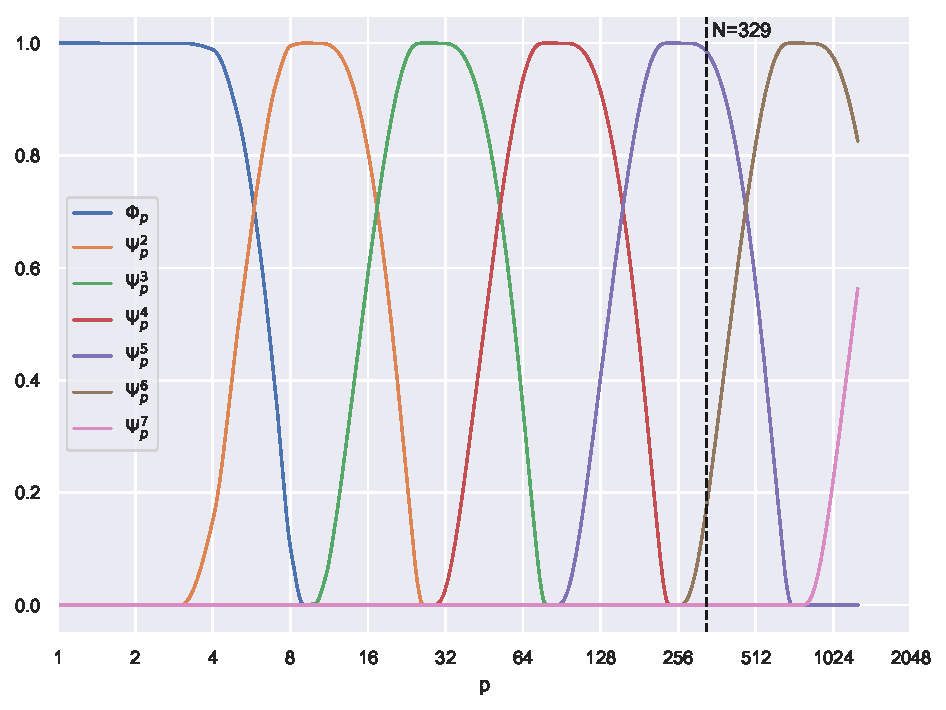
\includegraphics[width=\textwidth]{homer_slepian_tiling_b1275.pdf}
	\caption{
	}\label{fig:chapter4_tiling}
\end{figure}


\subsection{Properties}\label{sec:chapter4_properties}

The properties of Slepian wavelets on manifolds are reviewed here.
In comparison to standard scale-discretised wavelets, the properties are often similar, but not always.

\subsubsection{Localisation}\label{sec:chapter4_localisation}

A tiling of the harmonic line leads to the usual construction of scale-discretised wavelets.
Hence, the value of \(j\) in the wavelets \(\Psi^{j}\) corresponds to increasingly smaller scales (higher frequencies).
However, in the Slepian setting \(p\) is a measure of spatial concentration, where a lower \(p\) corresponds to better localisation of the Slepian function.
As Slepian wavelets are built on a tiling of the Slepian harmonic line, the localisation is captured in the wavelets and wavelet coefficients.

\subsubsection{Wavelet Energy}

The wavelet energy is
%
\begin{equation}
	\norm{\Psi^{j}}^{2}
	%
	= \integrateManifold{x} \abs{\mesh{\Psi^{j}}}^{2}
	%
	= \slepianSum \abs{\slepian{\Psi}^{j}}^{2}.
\end{equation}
%
Similarly, the scaling function energy is
%
\begin{equation}
	\norm{\Phi}^{2}
	%
	= \slepianSum \abs{\slepian{\Phi}}^{2}.
\end{equation}

\subsubsection{Parseval Frame}

A \emph{Parseval frame} is satisfied by Slepian scale-discretised wavelets on manifolds
%
\begin{equation}
	A\norm{f}^{2} \leq \integrateManifold{x} \bigg(
	%
	\abs{\braket{\translation{x}\Phi}{f}}^{2}
	%
	+ \waveletSum \abs{\braket{\translation{x}\Psi^{j}}{f}}^{2}
	%
	\bigg) \leq B\norm{f}^{2},
\end{equation}
%
where \(A,\ B \in \realPosParam{}\).
Proving this requires the definition in Slepian space of the scaling coefficients \cref{eq:chapter4_slepian_scaling_p} and the wavelet coefficients \cref{eq:chapter4_slepian_wavelet_p}, along with the orthogonality of the Slepian functions \cref{eq:chapter4_orthogonality_manifold}
%
\begin{equation}
	\slepianSum \abs{\slepian{\Phi}}^{2} \abs{\slepian{f}}^{2}
	%
	+ \waveletSum \abs{\slepian{\Psi}^{j}}^{2} \abs{\slepian{f}}^{2}
	%
	= \norm{f}^{2},
\end{equation}
%
where the admissibility condition \cref{eq:chapter4_admissibility} results in the final equality.
Therefore, a Parseval frame holds for scale-discretised wavelets with \(A = B = 1\), which implies that the energy of \(f\) is conserved in wavelet space.

\subsubsection{Wavelet Domain Variance}

For notational brevity define a quantity
%
\begin{equation}
	\varphi \in \set{\Phi,\Psi^{j}}
\end{equation}
%
to represent both the scaling function and the wavelets.
The variance of the wavelet/scaling coefficients is given by
%
\begin{equation}
	\variance{\mesh{W^{\varphi}}}
	%
	= \expval{\abs{\mesh{W^{\varphi}}}^{2}}
	%
	-\abs{\expval{\mesh{W^{\varphi}}}}^{2},
\end{equation}
%
where the expected value of the wavelet/scaling coefficients is zero for the common case of zero-mean Gaussian noise.
Thus, the variance can be expanded to become
%
\begin{equation}\label{eq:chapter4_slepian_isotropic_noise}
	\variance{\mesh{W^{\varphi}}}
	%
	= \slepianSum \slepianSum['] \slepian{\varphi} \slepian[']{\varphi} \mesh{\slepian{S}} \mesh{\slepian[']{S}} \expval{\slepian{f} \slepian[']{f}}.
\end{equation}

Consider homogenous and isotropic noise defined by its power spectrum
%
\begin{equation}
	\expval{f_{i} f_{j}}
	%
	= C_{i} \delta_{i j},
\end{equation}
%
where \(C_{i} = \sigma^{2}\) for white noise.
The power expression in Slepian space can be found by
%
\begin{align}
	\expval{\slepian{f} \slepian[']{f}}
	%
	 & = \sum\limits_{i} \sum\limits_{j} \expval{f_{i} f_{j}} \empty{} {(\slepian{S})}_{i} {(\slepian[']{S})}_{j} \nonumber \\
	%
	 & = \sigma^{2} \delta_{pp'},
\end{align}
%
where the first line follows from \cref{eq:chapter4_harmonic_to_slepian}, and the last line follows from the orthogonality of the Slepian functions \cref{eq:chapter4_orthogonality_manifold}.
Hence, the final expression for the wavelet domain variance is
%
\begin{equation}
	\variance{\mesh{W^{\varphi}}}
	%
	= \sigma^{2} \slepianSum \abs{\slepian{\varphi}}^{2} \abs{\mesh{\slepian{S}}}^{2},
\end{equation}
%
and as such the variance depends on the position on the manifold.

\section{Numerical Illustration}

In this section the construction and application of Slepian wavelets for an example region on a mesh (\cf{} manifold) is demonstrated.
The Slepian functions and eigenvalues of a region of a Homer Simpson mesh are presented in \cref{sec:chapter4_homer_region}.
A field is constructed on the region of the mesh in \cref{sec:chapter4_wavelet_transform}, and the resulting wavelets and wavelet coefficients are computed.
A possible use of Slepian wavelets is shown in \cref{sec:chapter4_wavelet_denoising} through a straightforward denoising procedure.
All computations are performed with the \texttt{S2LET}\footnote{\url{http://astro-informatics.github.io/s2let/}}~\cite{Leistedt2013} code, which enables the construction of the wavelet generating functions discussed in \cref{sec:chapter4_generating_functions}.

\subsection{Homer Region}\label{sec:chapter4_homer_region}

A region of a manifold is created on a mesh of Homer Simpson, \cref{fig:chapter4_homer_region} presents the masked region of Homer's head.
The Slepian functions of this region are computed by solving the eigenproblem \cref{eq:chapter4_eigenproblem}, and then performing an inverse harmonic transform.
The resulting Shannon number \cref{eq:chapter4_shannon} of the region \(R\) is \(N=329\).
A set of Slepian functions of the mesh are shown in \cref{fig:chapter4_slepian_functions} for \(p \in \set{1, 10, 25, 50, 100, 200}\).
Comparing panel (f) to panel (a) one can see that the latter Slepian functions are more spread out in the region, representing worse concentration.
The corresponding eigenvalues \(\slepian{\mu}\) are a measure of spatial concentration, which remain \(\almost{1}\) for many \(p\) values before rapidly decreasing towards zero around \(N\).
The first \(N\) eigenvalues of this Homer region are shown in \cref{fig:chapter4_slepian_eigenvalues}, were the plot to extend to all \(\imax{}\) Slepian eigenvalues then the rest of the eigenvalues would be \(\almost{0}\).

\begin{figure}[htp]
	\centering\capstart{}
	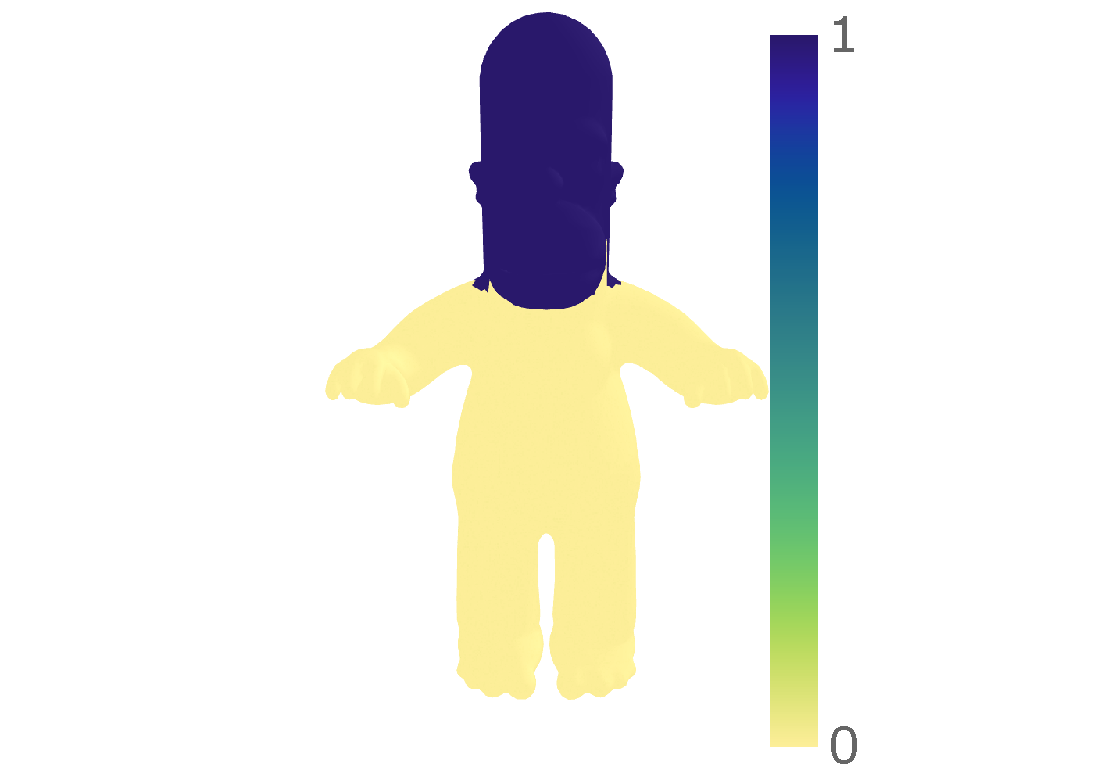
\includegraphics[trim={156 8 21 6},clip,width=.7\textwidth]{homer_region_norm.pdf}
	\caption[
		The head region of the Homer mesh
	]{
		The head region (in blue) chosen to compute the Slepian functions of the Homer mesh.
	}\label{fig:chapter4_homer_region}
\end{figure}


\begin{figure}[htp]
	\centering
	\subfloat[\(\mesh{S_{1}},\ \mu=1.00\)]
	{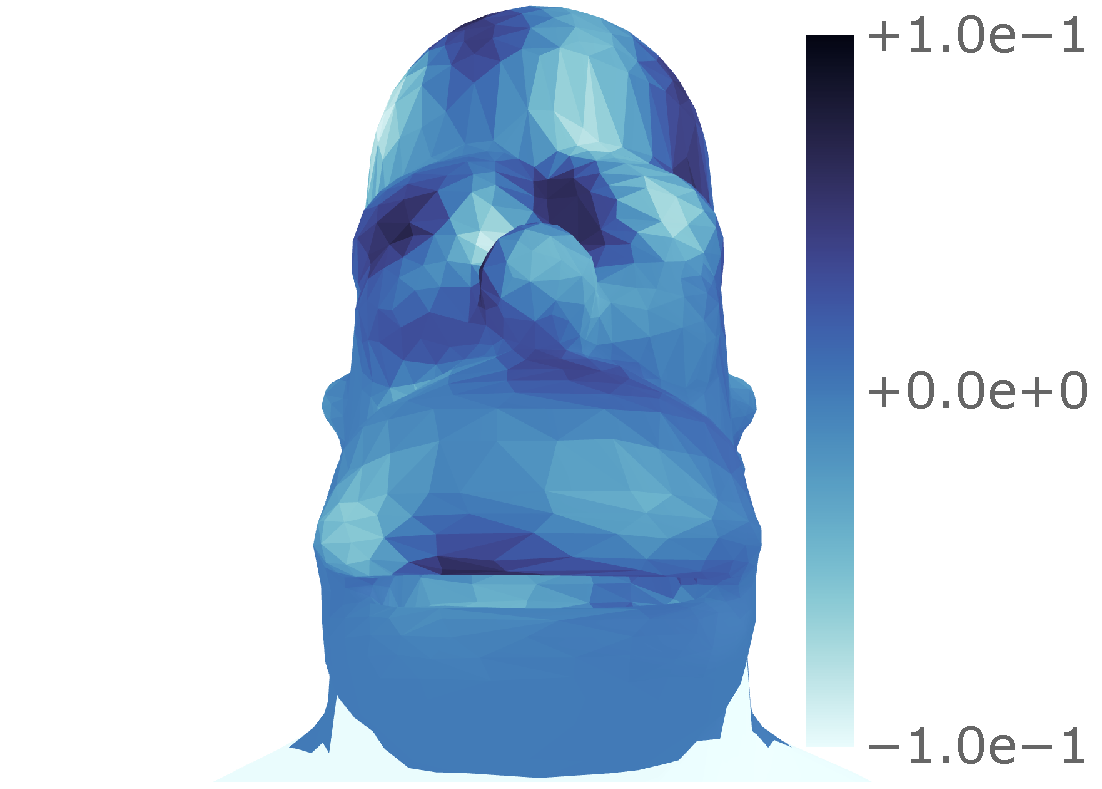
\includegraphics[trim={101 0 3 3},clip,width=.33\textwidth]{slepian_homer_rank0_lam1-000000e00_zoom.pdf}} % chktex 8
	\hfill
	\subfloat[\(\mesh{S_{10}},\ \mu=1.00\)]
	{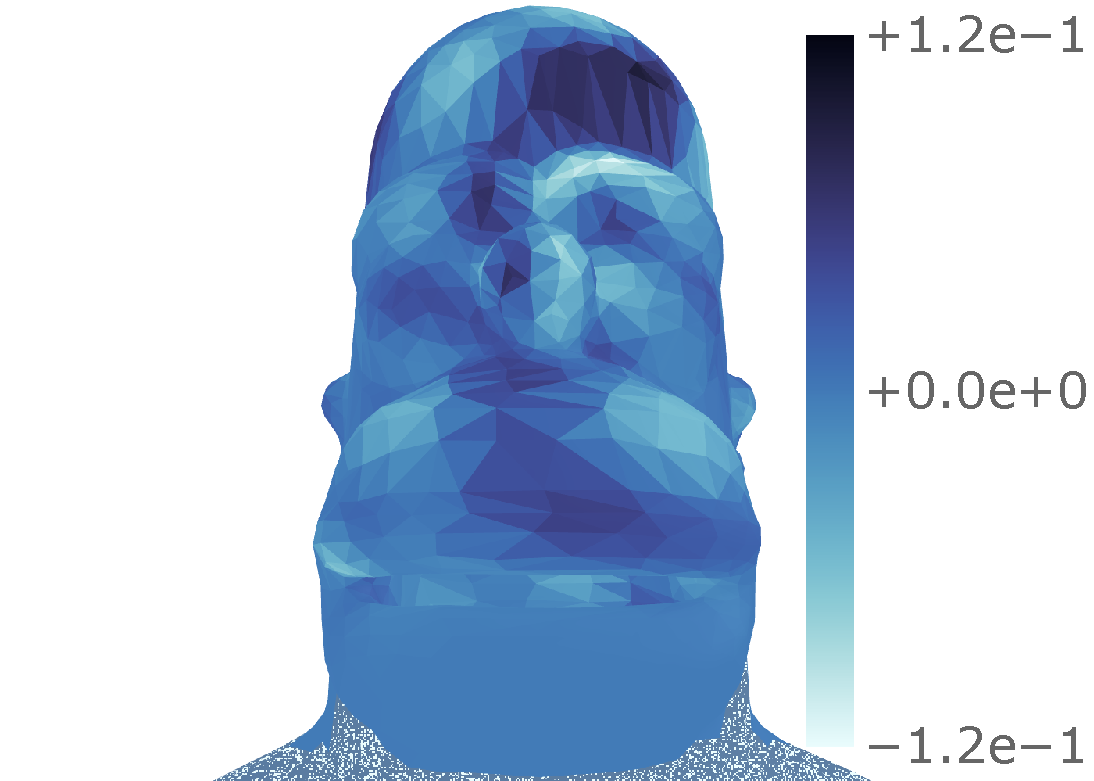
\includegraphics[trim={101 0 3 3},clip,width=.33\textwidth]{slepian_homer_rank9_lam1-000000e00_zoom.pdf}} % chktex 8
	\hfill
	\subfloat[\(\mesh{S_{25}},\ \mu=1.00\)]
	{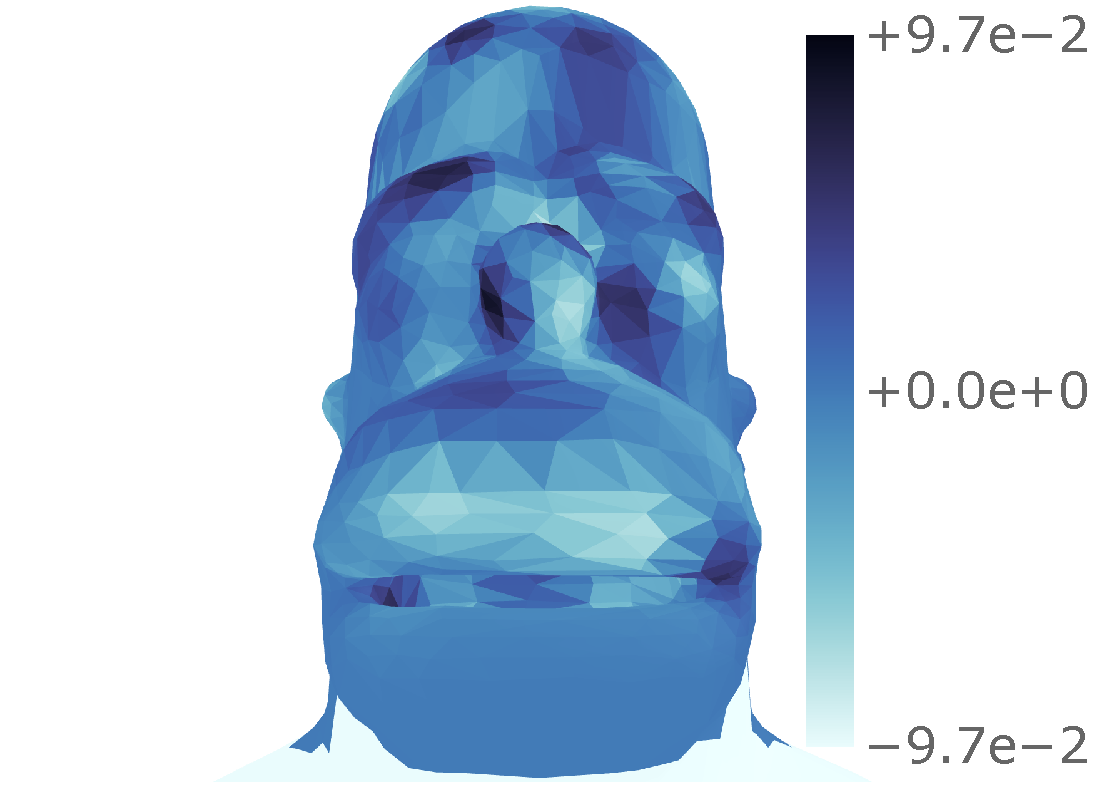
\includegraphics[trim={101 0 3 3},clip,width=.33\textwidth]{slepian_homer_rank24_lam1-000000e00_zoom.pdf}} % chktex 8
	\newline
	\subfloat[\(\mesh{S_{50}},\ \mu=1.00\)]
	{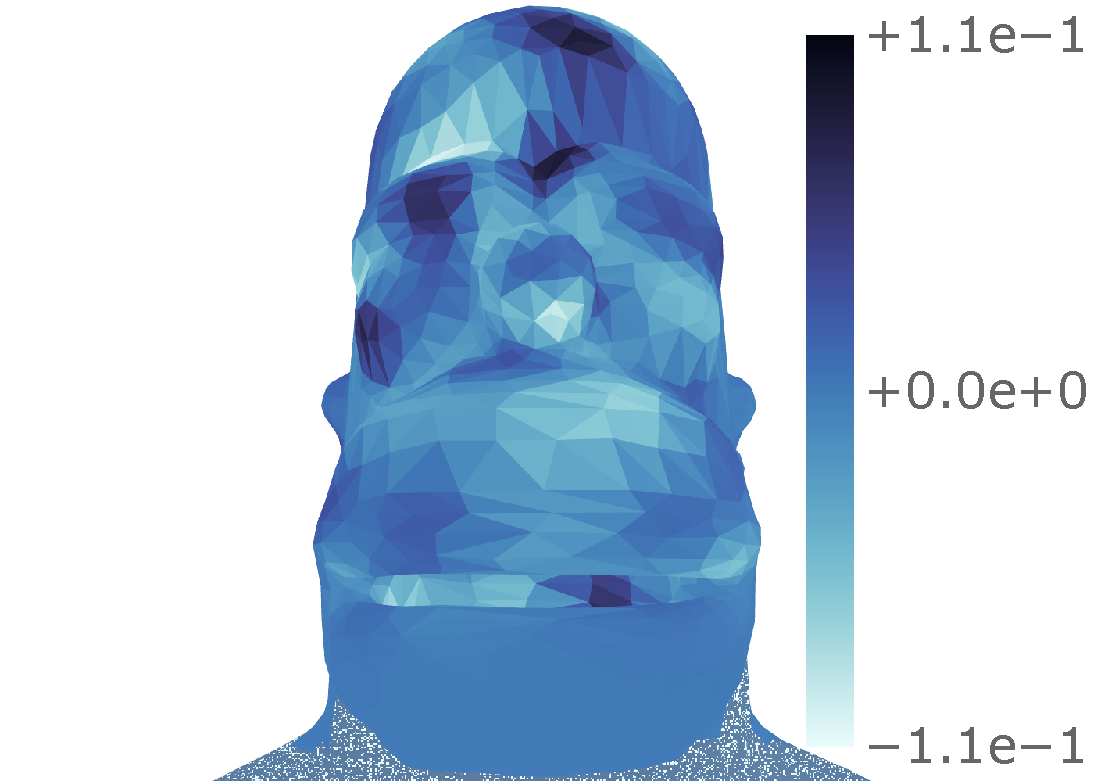
\includegraphics[trim={101 0 3 3},clip,width=.33\textwidth]{slepian_homer_rank49_lam1-000000e00_zoom.pdf}} % chktex 8
	\hfill
	\subfloat[\(\mesh{S_{100}},\ \mu=1.00\)]
	{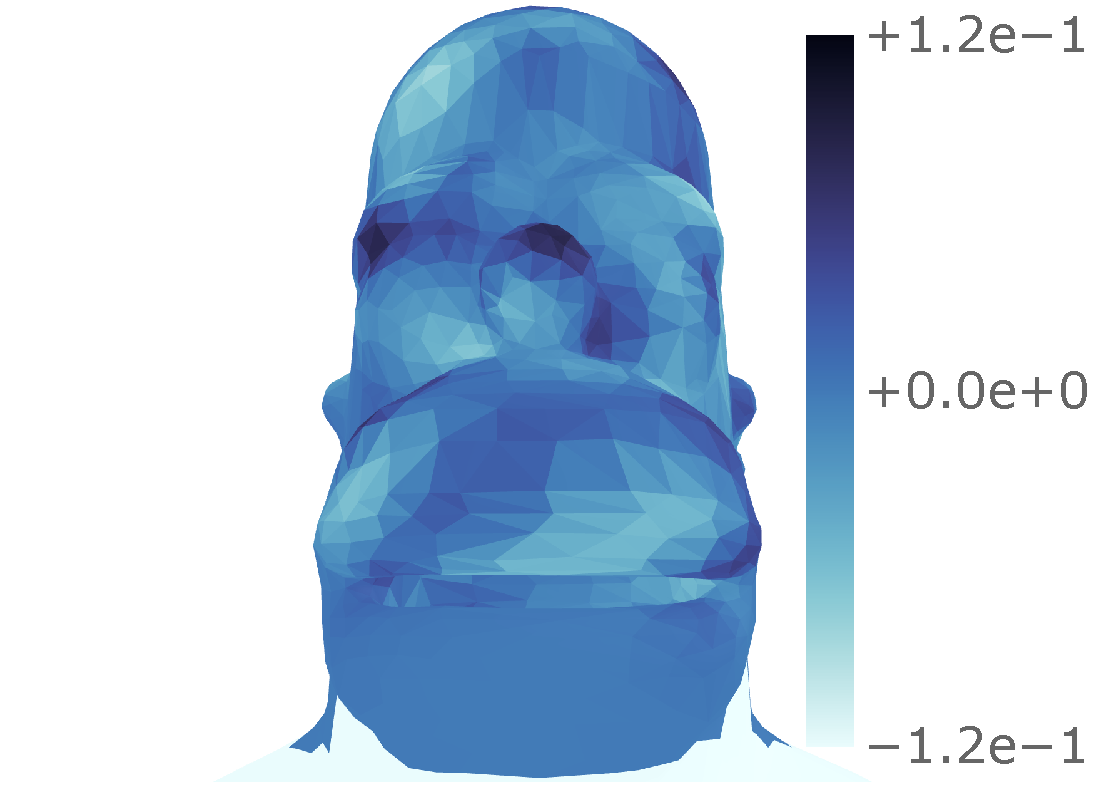
\includegraphics[trim={101 0 3 3},clip,width=.33\textwidth]{slepian_homer_rank99_lam1-000000e00_zoom.pdf}} % chktex 8
	\hfill
	\subfloat[\(\mesh{S_{200}},\ \mu=1.00\)]
	{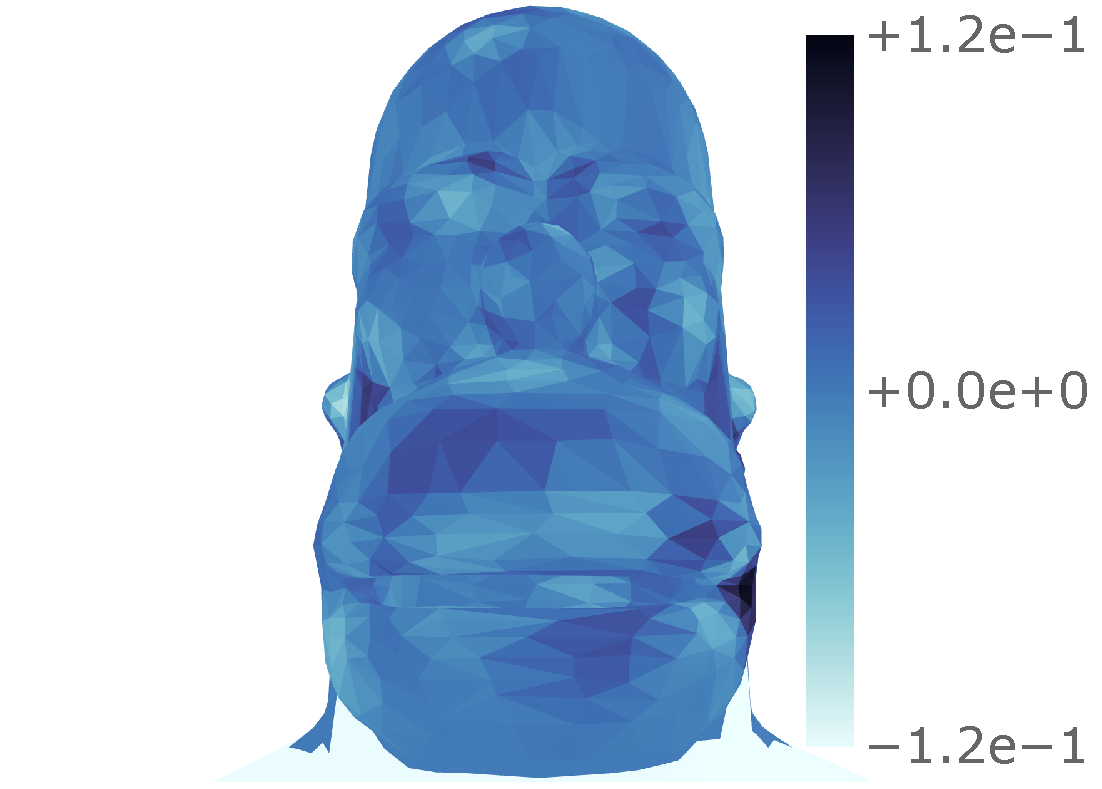
\includegraphics[trim={101 0 3 3},clip,width=.33\textwidth]{slepian_homer_rank199_lam1-000000e00_zoom.pdf}} % chktex 8
	\caption[
		Some Slepian functions of the Homer head region
	]{
		The Slepian functions of the Homer head region \(\mesh{\slepian{S}}\) for \(p \in \set{1, 10, 25, 50, 100, 200}\) shown left-to-right, top-to-bottom.
		The corresponding eigenvalue \(\slepian{\mu}\) is a measure of the concentration within the given region \(R\), which remains \(\almost{1}\) for many \(p\) values before decreasing towards zero.
		Whilst the Slepian functions are defined on the vertices, the values have been averaged onto the faces for the plot.
	}\label{fig:chapter4_slepian_functions}
\end{figure}


\begin{figure}[htp]
	\centering\capstart{}
	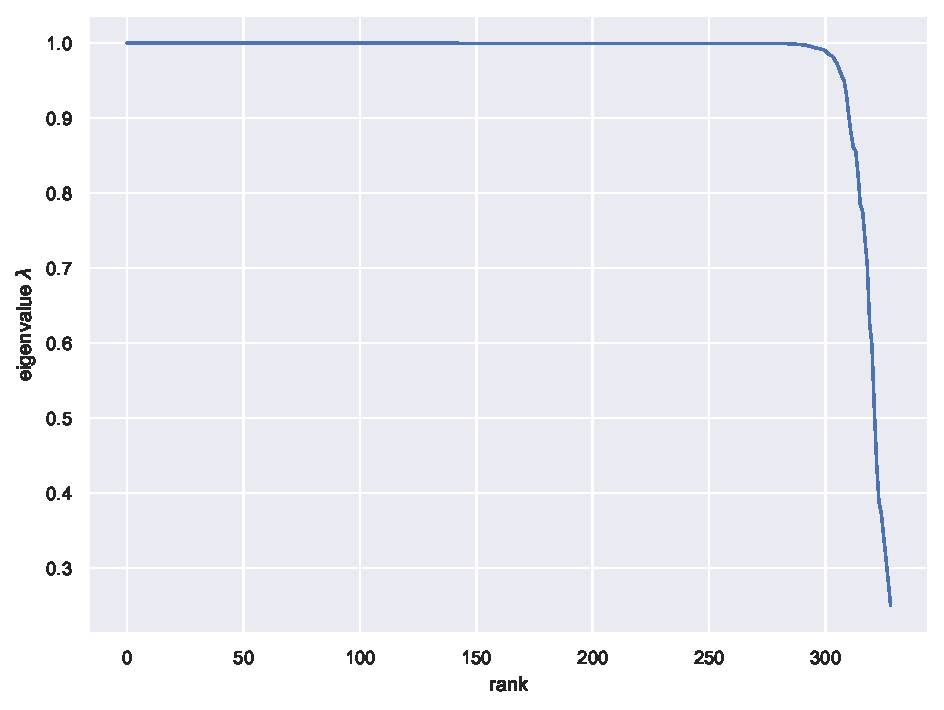
\includegraphics[width=\textwidth]{homer_slepian_eigenvalues_b1275.pdf}
	\caption[
		The Slepian eigenvalues of the Homer head region
	]{
		The eigenvalues of the Homer head region concentrated within the Shannon number \(N=329\).
		The majority of the eigenvalues are \(\almost{1}\) before decreasing rapidly towards zero around the Shannon number.
	}\label{fig:chapter4_slepian_eigenvalues}
\end{figure}


\subsection{Wavelet Transform}\label{sec:chapter4_wavelet_transform}

The Slepian scaling function and wavelets defined in \cref{sec:chapter4_slepian_scale_discretised_wavelets} are built on a tiling of the Slepian line with parameters \(\lambda=3\) and \(J_{0}=2\).
This tiling is shown in \cref{fig:chapter4_tiling} for \(\num{1275}\) basis functions of the Homer mesh, where the Shannon number \(N=329\) is highlighted.
Hence, for this region the scaling function and wavelets for scales \(j \in \set{2, 3, 4, 5, 6}\) are the only non-zero functions.
These wavelets are presented in \cref{fig:chapter4_wavelets}, which show a similar pattern to the Slepian functions where the scaling function is more concentrated in the region than the wavelet scale \(j=6\).
To perform a scale-discretised wavelet transform one requires a signal on the mesh.
\cref{fig:chapter4_homer_data} presents the such a signal, the \(z\)-component of the per vertex normals of the Homer mesh.
With some data to hand, the scaling and wavelet coefficients of the Homer head region are given in \cref{fig:chapter4_wavelet_coefficients}.

\begin{figure}[htp]
	\centering\capstart
	\subfloat[\(\mesh{\Phi}\)]
	{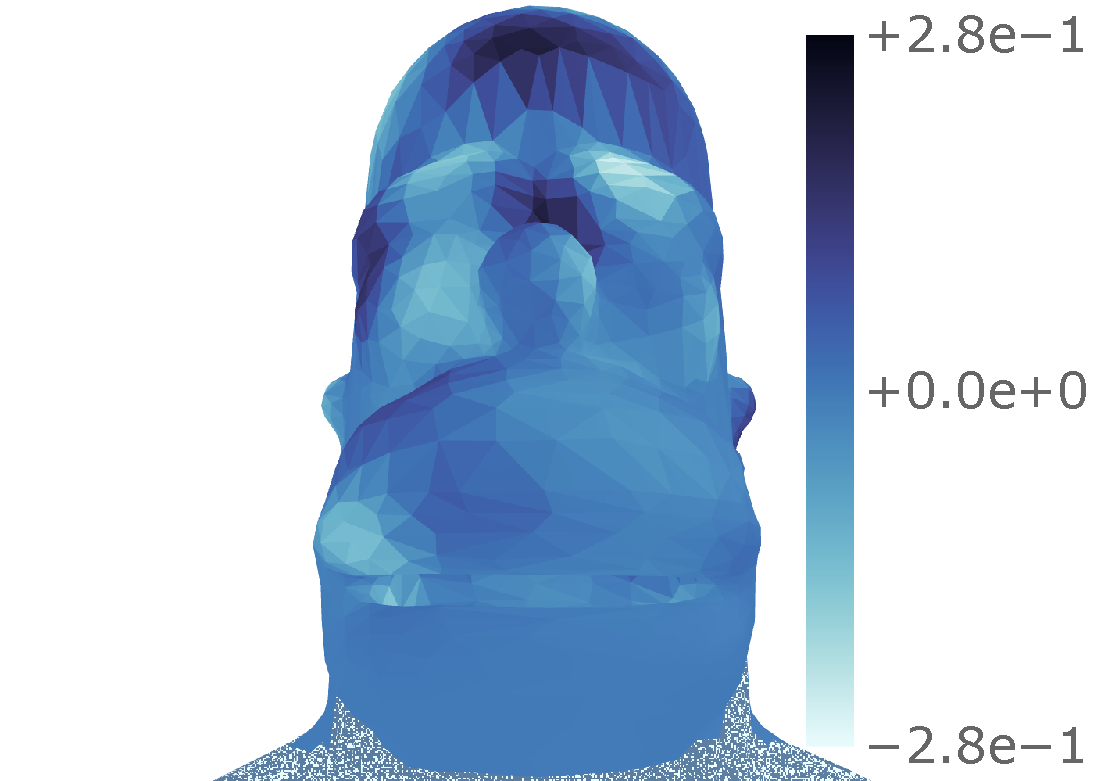
\includegraphics[trim={101 0 3 3},clip,width=.33\textwidth]{slepian_wavelets_homer_3B_2jmin_scaling_zoom.pdf}}
	\hfill
	\subfloat[\(\mesh{\Psi^{2j}}\)]
	{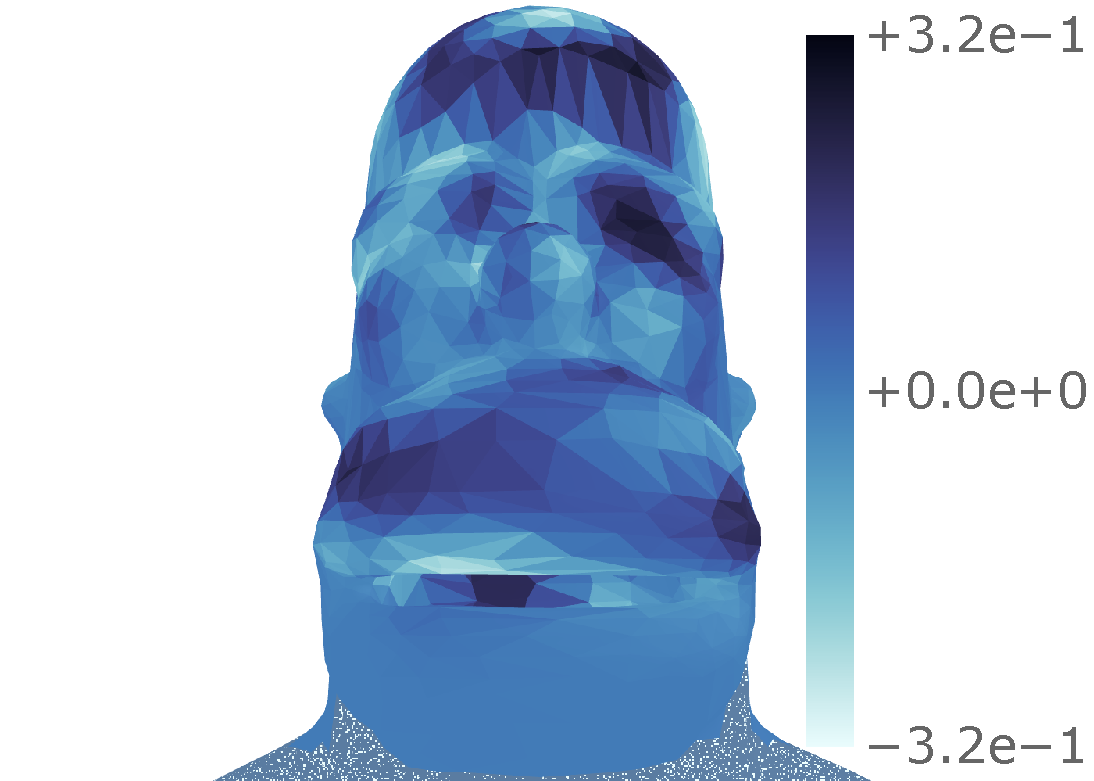
\includegraphics[trim={101 0 3 3},clip,width=.33\textwidth]{slepian_wavelets_homer_3B_2jmin_2j_zoom.pdf}}
	\hfill
	\subfloat[\(\mesh{\Psi^{3j}}\)]
	{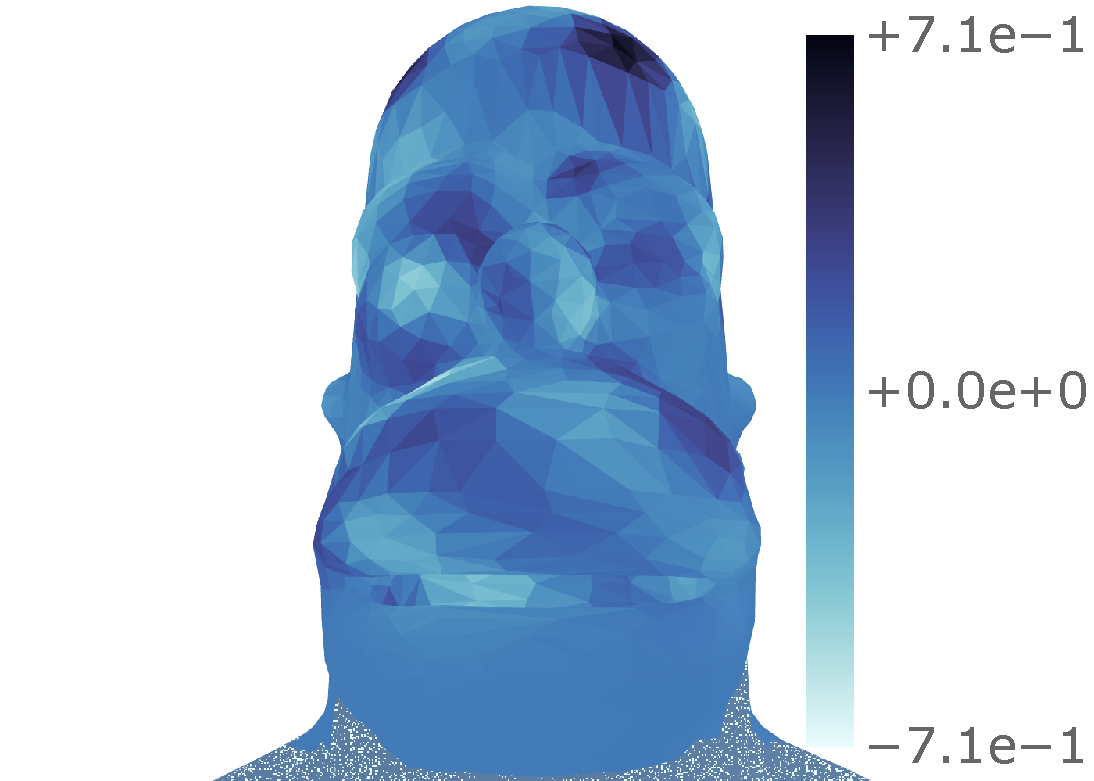
\includegraphics[trim={101 0 3 3},clip,width=.33\textwidth]{slepian_wavelets_homer_3B_2jmin_3j_zoom.pdf}}
	\newline
	\subfloat[\(\mesh{\Psi^{4j}}\)]
	{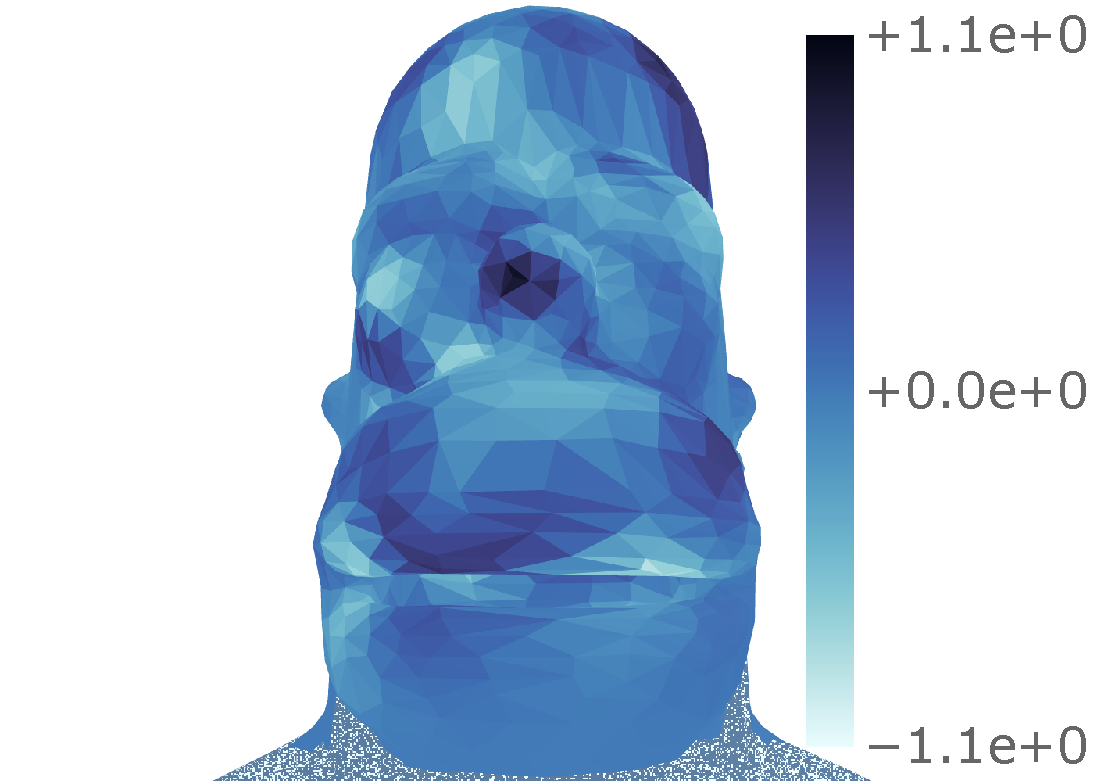
\includegraphics[trim={101 0 3 3},clip,width=.33\textwidth]{slepian_wavelets_homer_3B_2jmin_4j_zoom.pdf}}
	\hfill
	\subfloat[\(\mesh{\Psi^{5j}}\)]
	{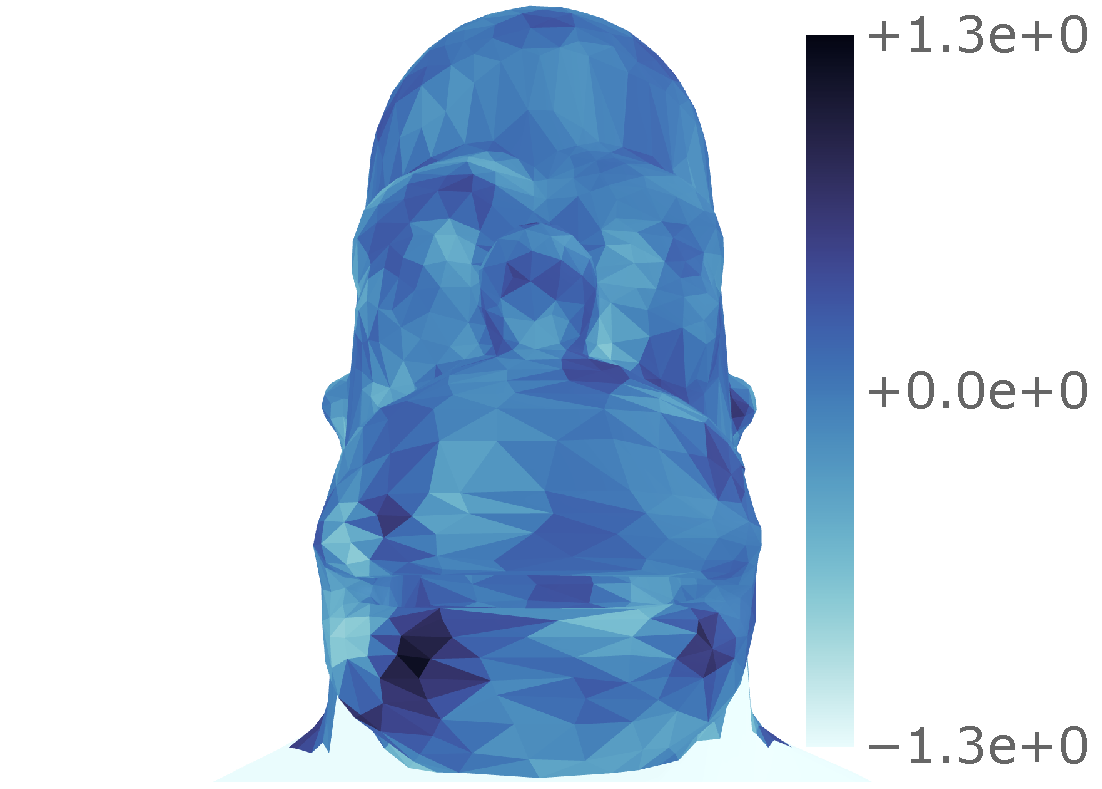
\includegraphics[trim={101 0 3 3},clip,width=.33\textwidth]{slepian_wavelets_homer_3B_2jmin_5j_zoom.pdf}}
	\hfill
	\subfloat[\(\mesh{\Psi^{6j}}\)]
	{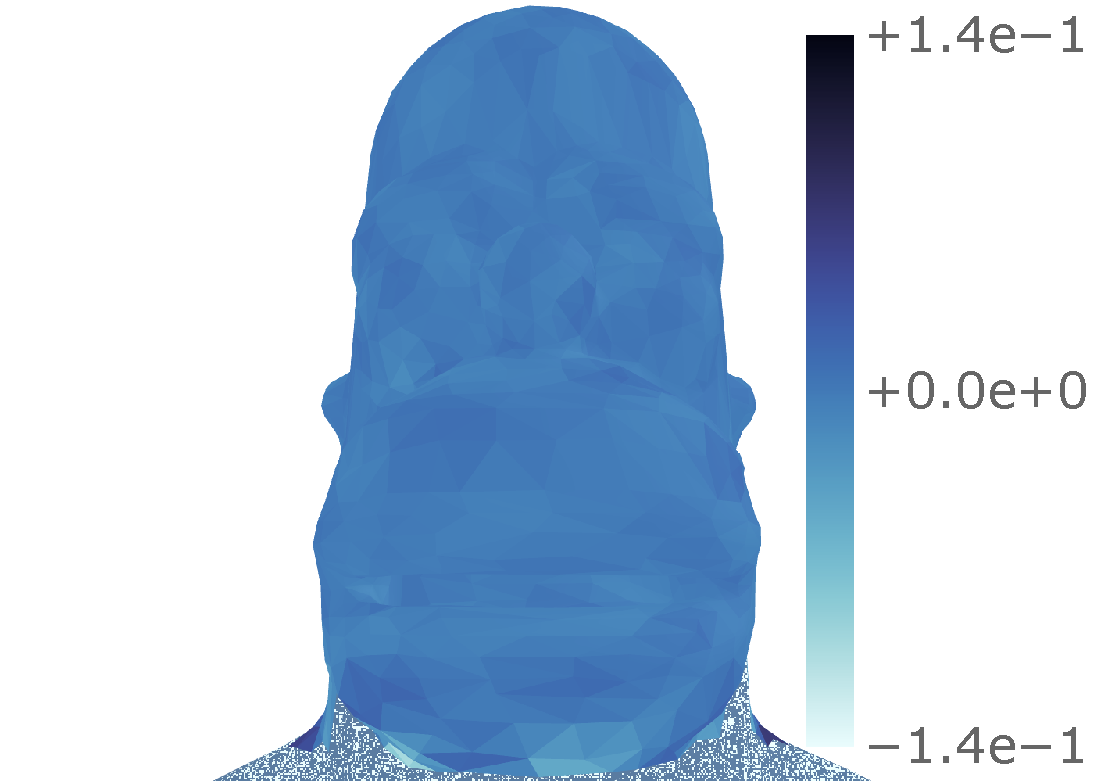
\includegraphics[trim={101 0 3 3},clip,width=.33\textwidth]{slepian_wavelets_homer_3B_2jmin_6j_zoom.pdf}}
	\caption[
		The Slepian wavelets of the Homer head region
	]{
		The scaling function and the wavelets for scales \(j \in \set{2, 3, 4, 5, 6}\) for the Homer head region shown left-to-right, top-to-bottom.
		The wavelets are constructed through a tiling of the Slepian line using scale-discretised functions, with parameters \(\lambda=3\), \(J_{0}=2\), and \(\imax=\num{1275}\) basis functions.
		Whilst the wavelets are defined on the vertices, the values have been averaged onto the faces for the plot.
	}\label{fig:chapter4_wavelets}
\end{figure}


\begin{figure}[htpb]
	\centering\capstart{}
	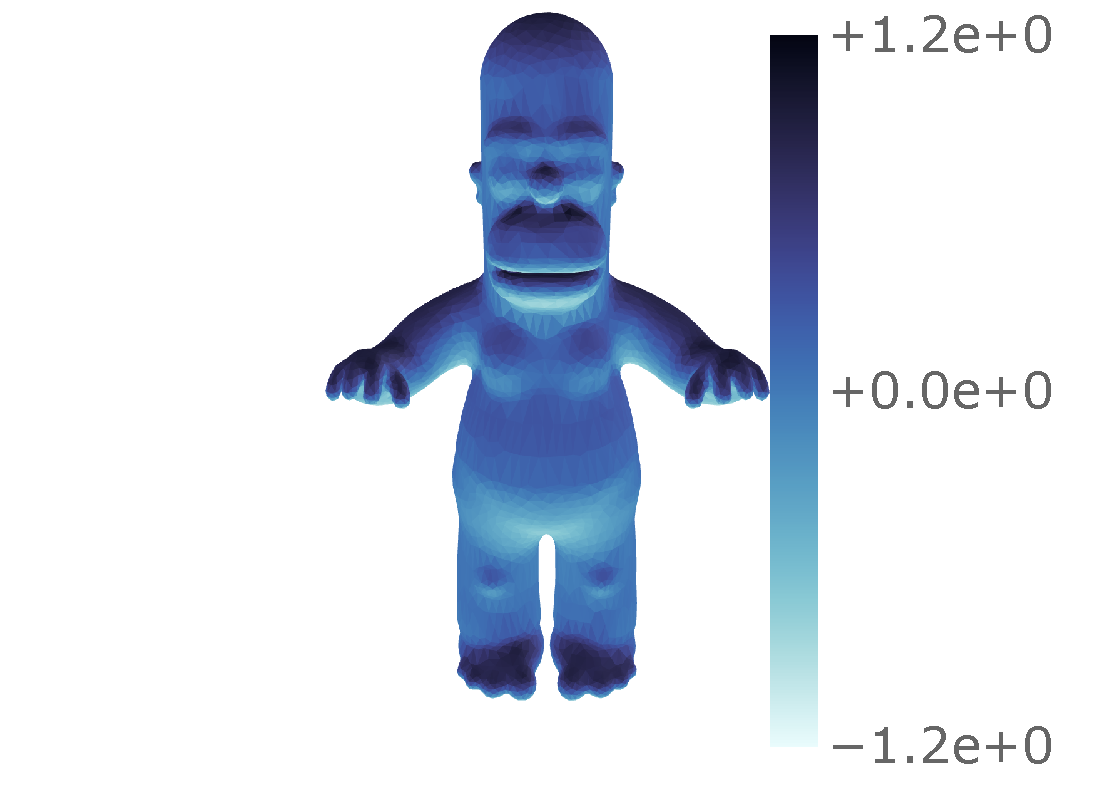
\includegraphics[trim={156 8 21 6},clip,width=.7\textwidth]{homer_field.pdf}
	\caption[
		An example field on the Homer mesh
	]{
		The \(z\)-component of the per vertex normals of the Homer mesh.
		Whilst the field is defined on the vertices, the values have been averaged onto the faces for the plot.
	}\label{fig:chapter4_homer_data}
\end{figure}


\begin{figure}[htp]
	\centering
	\subfloat[\(\mesh{W^{\Phi}}\)]
	{\includegraphics[trim={101 0 3 3},clip,width=.33\textwidth]{slepian_wavelet_coefficients_homer_3B_2jmin_scaling_zoom.pdf}}
	\hfill
	\subfloat[\(\mesh{W^{\Psi^{2j}}}\)]
	{\includegraphics[trim={101 0 3 3},clip,width=.33\textwidth]{slepian_wavelet_coefficients_homer_3B_2jmin_2j_zoom.pdf}}
	\hfill
	\subfloat[\(\mesh{W^{\Psi^{3j}}}\)]
	{\includegraphics[trim={101 0 3 3},clip,width=.33\textwidth]{slepian_wavelet_coefficients_homer_3B_2jmin_3j_zoom.pdf}}
	\newline
	\subfloat[\(\mesh{W^{\Psi^{4j}}}\)]
	{\includegraphics[trim={101 0 3 3},clip,width=.33\textwidth]{slepian_wavelet_coefficients_homer_3B_2jmin_4j_zoom.pdf}}
	\hfill
	\subfloat[\(\mesh{W^{\Psi^{5j}}}\)]
	{\includegraphics[trim={101 0 3 3},clip,width=.33\textwidth]{slepian_wavelet_coefficients_homer_3B_2jmin_5j_zoom.pdf}}
	\hfill
	\subfloat[\(\mesh{W^{\Psi^{6j}}}\)]
	{\includegraphics[trim={101 0 3 3},clip,width=.33\textwidth]{slepian_wavelet_coefficients_homer_3B_2jmin_6j_zoom.pdf}}
	\caption{
	}\label{fig:chapter4_wavelet_coefficients}
\end{figure}


\subsection{Wavelet Denoising}\label{sec:chapter4_wavelet_denoising}

Wavelets are used in a variety of contexts in signal processing, one common use case is for denoising a signal.
Localised features in the data can be extracted to different wavelet scales, and hence the desired parts of the signal can be preserved whilst isolating the noise.
To showcase Slepian wavelets, white noise is added to the signal in the right panel of \cref{fig:chapter4_homer_data}.
A straightforward hard-thresholding denoising procedure follows.

Consider a signal localised in the region \(R\) in the presence of noise
%
\begin{equation}\label{eq:chapter4_noised_signal}
	\mesh{z}
	%
	= \mesh{s} + \mesh{n},
\end{equation}
%
where the signal and noise are represented by \(\mesh{s}\) and \(\mesh{n}\) respectively.
The power spectrum of noise in Slepian space is as before
%
\begin{equation}
	\expval{\slepian{n} \slepian[']{n}}
	%
	= \sigma^{2} \delta_{pp'}.
\end{equation}
%
To assess the recovery of the initial data, a signal-to-noise ratio for the region is defined
%
\begin{equation}
	\snr{z}
	%
	\equiv 10 \log_{10} \frac{\norm{s}^{2}}{\norm{z - s}^{2}}.
\end{equation}
%
A denoised version of \(z\) is desired, denoted by \(d \in \hilbert{R}\), with a large \(\snr{d}\) such that \(d\) extracts the informative signal \(s\).
Often the scaling coefficients are \emph{not} used in hard-thresholding; however, in the Slepian setting the scaling function and wavelets are treated equivalently.
The scaling function in the Slepian setting is not a low-frequency representation of the signal due to the localisation of the Slepian functions (see \cref{sec:chapter4_localisation}).

Since the wavelet transform is linear, the individual elements sum to give the wavelet/scaling coefficients of \cref{eq:chapter4_noised_signal}
%
\begin{equation}
	\mesh{Z^{\varphi}}
	%
	= \mesh{S^{\varphi}} + \mesh{N^{\varphi}},
\end{equation}
%
where the wavelet coefficients are denoted by capital letters, \ie{}
%
\begin{equation}
	\mesh{Z^{\varphi}} = \mesh{\convolution{\varphi}{z}}.
\end{equation}
%
In wavelet space the noise is
%
%
\begin{equation}
	\variance{\mesh{N^{\varphi}}}
	%
	= \sigma^{2} \slepianSum \abs{\slepian{\varphi}}^{2} \abs{\mesh{\slepian{S}}}^{2}
	%
	\equiv {\mesh{\sigma^{\varphi}}}^{2},
\end{equation}
%
where \(\sigma^{\varphi}\) represents the standard deviation of the noise in wavelet space.
To denoise the signal one may hard-threshold the scaling/wavelet coefficients with a threshold \(T\) proportional to the standard deviation of the noise.
Hence, the denoised wavelet coefficients \(\mesh{D^{\varphi}} = \mesh{\convolution{\varphi}{d}}\) are
%
\begin{equation}
	\mesh{D^{\varphi}} =
	%
	\begin{cases}
		0,
		%
		 & \mesh{Z^{\varphi}} < \mesh{T^{\varphi}},    \\
		%
		\mesh{Z^{\varphi}},
		%
		 & \mesh{X^{\varphi}} \geq \mesh{T^{\varphi}},
	\end{cases}
\end{equation}
%
where
%
\begin{equation}
	\mesh{T^{\varphi}}
	%
	= N_{\sigma}\mesh{\sigma^{\varphi}},
\end{equation}
%
with \(N_{\sigma} \in \realPosParam{}\).
Reconstruction of the signal \(d\) follows by an inverse wavelet transform with these thresholded wavelet coefficients.
This procedure merely demonstrates a practical use case of Slepian wavelets, more sophisticated denoising formalisms can be developed.

To perform the denoising, Gaussian white noise is added to the data in the right panel of \cref{fig:chapter4_homer_data}.
The noised signal is shown in panel (a) of \cref{fig:chapter4_denoising} with an initial signal-to-noise ratio of \(\SI{0.32}{\dB}\).
Panels (b-c) show the results of the denoising procedure describe above for \(N_{\sigma} \in \set{1,2}\), with signal-to-noise ratios of \(\SI{2.29}{\dB}\) and \(\SI{0.98}{\dB}\) respectively.
At \(N_{\sigma}=1\) an initial boost in signal-to-noise ratio is observed; however, as more signal is removed the hard-thresholding scheme experiences diminishing returns.

The same denoising procedure was conducted for a series of other meshes, the Slepian regions of which are shown in \cref{fig:chapter4_other_meshes}.
These meshes are comparable in size to the \(\num{5103}\) vertex Homer mesh, and an appropriate region \(R\) has been highlighted in black for each.
\cref{tab:chapter4_denoising} presents the Shannon number, the number of non-zero wavelets, and the denoising results for each mesh for the same wavelet parameters as before --- \(\lambda=3\) and \(J_{0}=2\).
In general, the hard-thresholding scheme boosts the signal-to-noise ratio of the signal on the mesh, in particular for higher Shannon numbers (more wavelets).
Fine-tuning the wavelet parameters \(\lambda{}\) and \(J_{0}\) would result in a larger signal-to-noise boost for each mesh.

\begin{figure}[htp]
	\centering\capstart{}
	\subfloat[Initial Data]
	{\includegraphics[trim={101 0 3 3},clip,width=.33\textwidth]{slepian_homer_field_zoom.pdf}}
	\hfill
	\subfloat[Noisy Data \newline
		\(\snr{z} = \SI{0.32}{\dB}\)]
	{\includegraphics[trim={101 0 3 3},clip,width=.33\textwidth]{slepian_homer_field_-5noise_zoom.pdf}}
	\hfill
	\subfloat[Denoised \(N_{\sigma}=1\) \newline
		\(\snr{d} = \SI{2.29}{\dB}\)]
	{\includegraphics[trim={101 0 3 3},clip,width=.33\textwidth]{homer_-5snr_1n_denoised.pdf}}
	\caption[
		A denoising demonstration for a field on the Homer mesh
	]{
		Panel (a) shows the data in the region \(R\) constructed from the Slepian coefficients of the per vertex normals (\cf{} \cref{fig:chapter4_homer_data}) --- where the field value outside the region is set to negative infinity for illustrative purposes.
		Gaussian white noise is added to the signal in the Homer head region with a signal-to-noise ratio of \(\SI{0.32}{\dB}\), shown in panel (b).
		The scaling and wavelet coefficients of the noisy signal are calculated and are then hard-thresholded with \(N_{\sigma}=1\).
		The corresponding denoised plot is shown in panel (c), where the signal-to-noise ratio is boosted by \(\SI{1.97}{\dB}\) to \(\SI{2.29}{\dB}\).
		Whilst the signal values are defined on the vertices, they have been averaged onto the faces for the plot.
	}\label{fig:chapter4_denoising}
\end{figure}


\begin{figure}[htp]
	\centering
	\subfloat[Bird]
	{\includegraphics[trim={7 8 3 7},clip,width=.38\textwidth]{bird_region_norm.pdf}}
	\hfill
	\subfloat[Cheetah]
	{\includegraphics[trim={137 1 3 7},clip,width=.28\textwidth]{cheetah_region_norm.pdf}}
	\hfill
	\subfloat[Cube]
	{\includegraphics[trim={62 1 3 7},clip,width=.33\textwidth]{cube_region_norm.pdf}}
	\newline
	\subfloat[Dragon]
	{\includegraphics[trim={75 8 3 7},clip,width=.33\textwidth]{dragon_region_norm.pdf}}
	%
	\subfloat[Teapot]
	{\includegraphics[trim={3 8 3 7},clip,width=.38\textwidth]{teapot_region_norm.pdf}}
	\caption{
		The Slepian regions (in black) of some other meshes.
		The same denoising procedure as in \cref{fig:chapter4_denoising} was performed for these alternative meshes, the results are shown in \cref{tab:chapter4_denoising}.
	}\label{fig:chapter4_other_meshes}
\end{figure}


\begin{table}
	\centering
	\caption{
		Denoising of other meshes.
	}\label{tab:chapter4_denoising}
	\begin{tabular}{@{}rcccc@{}}
		\toprule
		        & Shannon       & Wavelets    & Initial SNR         & \(N_{\sigma}=1\) SNR \\
		\midrule
		Cheetah & \(\num{72}\)  & \(\num{4}\) & \(\SI{3.96}{\dB}\)  & \(\SI{3.58}{\dB}\)   \\
		%
		Dragon  & \(\num{169}\) & \(\num{5}\) & \(\SI{3.44}{\dB}\)  & \(\SI{2.69}{\dB}\)   \\
		%
		Bird    & \(\num{194}\) & \(\num{5}\) & \(\SI{0.49}{\dB}\)  & \(\SI{1.59}{\dB}\)   \\
		%
		Teapot  & \(\num{256}\) & \(\num{6}\) & \(\SI{-1.57}{\dB}\) & \(\SI{-0.08}{\dB}\)  \\
		%
		Cube    & \(\num{272}\) & \(\num{6}\) & \(\SI{2.65}{\dB}\)  & \(\SI{3.85}{\dB}\)   \\
		%
		Homer   & \(\num{329}\) & \(\num{6}\) & \(\SI{0.32}{\dB}\)  & \(\SI{2.29}{\dB}\)   \\
		\bottomrule
	\end{tabular}
\end{table}


\section{Conclusions}\label{sec:chapter4_conclusions}

\chapter{Slepian Scale-Discretised Wavelets on Manifolds}\label{sec:chapter5}

Inspired by recent interest in geometric deep learning, this chapter generalises the recently developed Slepian scale-discretised wavelets on the sphere to Riemannian manifolds.
Through the sifting convolution, one may define translations and, thus, convolutions on manifolds --- which are otherwise not well-defined in general.
Slepian wavelets are constructed on a region of a manifold, and are therefore suited to problems where data only exists in a particular region.
The Slepian functions, on which Slepian wavelets are built, are the basis functions of the Slepian spatial-spectral concentration problem on the manifold.
A tiling of the Slepian harmonic line with smoothly decreasing generating functions defines the scale-discretised wavelets; allowing one to probe spatially localised, scale-dependent features of a signal.
By discretising manifolds as graphs, the Slepian functions and wavelets of a triangular mesh are presented.
Through a wavelet transform, the wavelet coefficients of a field defined on the mesh are found and used in a straightforward thresholding denoising scheme.

\section{Introduction}

Many fields measure data which are intrinsically non-Euclidean in structure and are better modelled by manifolds or graphs.
One manifold, in particular, which is in commonplace in science and engineering is the sphere; such as in: cosmology~\cite{Bennett1996}, geophysics~\cite{Simons2006}, planetary science~\cite{Turcotte1981}, computer graphics~\cite{Ramamoorthi2004}, and signal processing~\cite{Roddy2021a}.
Often data are not observed in some region of the manifold, and hence methods which work over the whole manifold may not be appropriate.
One such example, in the spherical setting, is in cosmic microwave background analyses where foreground microwave emissions dominate the region around the  Galactic plane and are often removed~\cite{Mortlock2002}.
Wavelets are a typical approach to deal with problems of this form, which allow the probing of spatially localised, scale-dependent features of the signal.
Contamination of the wavelet coefficients at the boundaries of the region, however, still presents a problem.
In \cref{sec:chapter4}, Slepian wavelets are constructed within a region of the sphere.
Here, in this chapter, Slepian wavelets are generalised to the manifold setting following an analogous construction.

In data analyses, one often desires to extract non-trivial patterns in the data.
By projecting the data onto an appropriate basis, patterns which were not considered before may present themselves.
If one seeks to find oscillatory features, then a Fourier basis is often most appropriate, \ie{} the spherical harmonics in the spherical setting.
Wavelets, however, simultaneously extract contributions of scale-dependent features in both space and scale.
Wavelets on the sphere (\cf{} manifold) have been applied in fields such as: astrophysics and cosmology~\cite{Pen1999,Barreiro2001,Rocha2004,McEwen2004}, planetary science~\cite{Audet2011,Audet2014}, and geophysics~\cite{Loris2010,Simons2011,Simons2011b}.
Scale-discretised wavelets (on the sphere)~\cite{Wiaux2008,McEwen2018,Leistedt2013,McEwen2013,McEwen2015} lean on a tiling of the harmonic line to produce an exact wavelet transform in both the continuous and discrete settings.

A new research direction, \emph{geometric deep learning}, has evolved from an increasing interest in non-Euclidean data geometries; where convolutional networks are generalised to graph and manifold structured data (\eg{}~\cite{Bronstein2017,Perlmutter2020}).
In general, geometric learning problems are split into two categories: characterising the structure of the data, and analysing functions defined on a non-Euclidean domain.
Manifold learning models (\eg{}~\cite{Tenenbaum2000,Coifman2006b,VanDerMaaten2008}) are a set of unsupervised algorithms which capture the intrinsic structure in the data through data-driven geometries.
Moreover, signals on manifolds are increasingly prevalent in areas such as shape matching and computer graphics.
Thus, many works are emerging to generalise spectral and signal processing methods to manifolds~\cite{Coifman2006} and graphs~\cite{Shuman2013}.
In these settings, functions are supported on the manifold/the vertices of the graph, and the Fourier harmonics are the eigenfunctions of the \emph{Laplace-Beltrami operator}/eigenvectors of the \emph{graph Laplacian}.

Graphs are a fundamental data structure, which are useful in describing geometric structures of data in domains such as: social~\cite{Nettleton2013}, transportation~\cite{Mohan2014}, sensor~\cite{Kenniche2010}, and neuronal~\cite{Tang2012} networks.
Each edge in a graph is associated with a weight, which is often a measure of the similarity between two connected vertices in a graph.
The physics of the problem or the data at hand dictate which vertices are connected and their respective weights, \ie{} the weight may not necessarily be the physical distance between two vertices.
A \emph{graph signal} is a finite collection of samples with some value at each vertex at a graph.
In computer graphics, working with intrinsically geometric shapes is commonplace.
In this field, three-dimensional shapes are often modelled as Riemannian manifolds and discretised as triangular meshes.

It is well-known that functions cannot have finite support in the spatial and spectral domains simultaneously~\cite{Slepian1961,Slepian1983}.
In the 1960s, Slepian, Landau and Pollak solved the fundamental problem of finding and representing signals which are optimally concentrated in both domains~\cite{Slepian1961,Landau1961,Landau1962}.
The \emph{Slepian spatial-spectral concentration problem} (or the \emph{Slepian concentration problem} for short) results in the families of functions which are optimally concentrated in the spatial (spectral) domain, and exactly limited in the spectral (spatial) domain.
The Slepian concentration problem was initially formed in the Euclidean domain; however, it has since been generalised to other geometries, such as: the sphere~\cite{Simons2006,Wieczorek2005,Albertella1999,Cohen1989,Meaney1984,Daubechies1988}, and graphs~\cite{VanDeVille2017,VanDeVille2017a,Bolton2018}.
The so-called \emph{Slepian functions} arise in many fields within science and engineering, such as: medical imaging~\cite{Jackson1991}, signal processing~\cite{Mathews1985,Thomson1982}, and geophysics~\cite{Thomson1976,Simons2006a,Simons2011}.
Notably, these functions have been used in interpolation~\cite{Moore2004,Shkolnisky2006}, extrapolation~\cite{Xu1983}, inverse problems~\cite{Villiers2001,Abdelmoula2015}, and solving partial differential equations~\cite{Boyd2003,Chen2005}.

Due to recent interest in geometric deep learning, many fields are extending existing methods developed in the Euclidean domain to manifolds or graphs, \ie{}~\cite{Perlmutter2020}.
This chapter generalises Slepian scale-discretised wavelets on the sphere~\cite{Roddy2021a} to Riemannian manifolds.
These wavelets constitute a basis designed for incomplete data on manifolds or graphs.
Here, the scale-discretised wavelet construction on the sphere~\cite{Wiaux2008,McEwen2018,Leistedt2013,McEwen2013,McEwen2015} is extended to the Slepian domain; however, the Slepian functions are now constructed on a region of a general manifold (rather than strictly the sphere).
As before, scale-discretised wavelets exhibit an explicit inversion formula, constitute a tight frame, and have excellent localisation properties in both spectral and spatial domains.
The wavelets themselves are constructed through a tiling of the Slepian harmonic line --- built from the eigenfunctions of the Slepian concentration problem on the manifold.
The wavelet transform follows through a generalisation of the \emph{sifting convolution}~\cite{Roddy2021}, discussed in \cref{sec:chapter3}, which allows one to perform convolutions on (incomplete) manifolds.
The wavelet construction is analogous to the spherical case, but with the eigenfunctions of the Laplace-Beltrami operator/eigenvectors of the graph Laplacian, rather than the spherical harmonics.

In \cref{sec:chapter4}, Slepian scale-discretised wavelets on the sphere~\cite{Roddy2021a} were introduced.
This chapter generalises these wavelets to Riemannian manifolds; however, Slepian wavelets have been considered before.
Multiresolution analyses have been performed with prolate spheroidal wave functions~\cite{Walter2004} in the Euclidean setting.
In spherical settings, spatially localised spherical harmonic transforms are sometimes used (\eg{}~\cite{Simons1997,Wieczorek2005,Khalid2013,Khalid2013a}).
Other times, the Slepian functions on the sphere are used directly~\cite{Simons2009}.
A variety of other approaches include: established regularisation techniques based on a known singular value decomposition~\cite{Michel2017}, and wavelet-like representations without explicit inverse transforms~\cite{Simons2011}.
Extending wavelets and wavelet techniques to manifold and graph domains has been extensively reviewed (\eg{}~\cite{Dahmen1999,Coifman2006a}).

The remainder of this chapter is as follows.
\cref{sec:chapter5_mathematical_background_problem_formulation} presents some mathematical preliminaries of Riemannian manifolds, their representations as graphs, and triangular meshes.
The Laplace-Beltrami operator and the graph/mesh Laplacian are also introduced.
A brief review of Slepian scale-discretised wavelets on the sphere~\cite{Roddy2021a} follows, which this works builds upon.
In \cref{sec:chapter5_working_with_manifolds} the Slepian concentration problem is adapted to the manifold setting, which results in the basis functions of a region of the manifold, \ie{} the Slepian functions.
A review of the sifting convolution~\cite{Roddy2021} follows, which allows one to perform convolutions on the (incomplete) manifold --- which are typically not well-defined.
The Slepian wavelet theory is developed in \cref{sec:chapter5_slepian_wavelets}.
Initially, the sifting convolution is expressed in the Slepian domain, which is a product in the Slepian harmonic space.
The scale-discretised framework is then introduced, followed by the generating functions which define the wavelets themselves.
The section concludes with some properties of the wavelets.
A numerical illustration is presented in \cref{sec:chapter5_numerical_illustration}, in which the Slepian functions of the head region of a triangular mesh of Homer Simpson are computed.
A field is then placed on the mesh, and the resulting wavelets and wavelet coefficients are found through a wavelet transform.
A straightforward hard-thresholding denoising scheme is developed and performed on the Homer mesh, along with some other meshes.
A boost in signal-to-noise ratio is observed, showcasing a possible use of these wavelets.
Lastly, some concluding remarks are given in \cref{sec:chapter5_conclusions}.

\section{Mathematical Background and Problem Formulation}\label{sec:chapter5_mathematical_background_problem_formulation}

Some mathematical preliminaries are introduced in \cref{sec:chapter5_mathematical_preliminaries} with a recap of Riemannian manifolds, their representation as graphs, and triangular meshes (a popular choice of graph).
This includes a review of the Laplace-Beltrami operator (on manifolds) and the graph/mesh Laplacian.
This chapter extends Slepian scale-discretised wavelets on the sphere to manifolds, a brief review of which is given in \cref{sec:chapter5_problem_formulation}.

\subsection{Mathematical Preliminaries}\label{sec:chapter5_mathematical_preliminaries}

\subsubsection{Riemannian Manifolds}

In short, a manifold is a space that is locally Euclidean.
For example, at a point on the surface of the Earth (\ie{} \(\twoSphere{}\)) the Earth's surface appears planar --- leading to the so-called \emph{Flat Earth} theory.
More formally, a \(d\)-dimensional manifold \(\manifold{}\) is a topological space, where each point \(x\) exists in a neighbourhood that is topologically homeomorphic to a \(d\)-dimensional Euclidean space --- called the \emph{tangent space}.
Let \(\manifold{}\) denote a compact, smooth, connected \(d\)-dimensional Riemannian manifold without boundary contained in \(\mathbb{R}^{n}\).
The Hilbert space \(\hilbert{\manifold}\) is formed by the set of functions \(f : \manifold \to \mathbb{R}\) that are square-integrable with respect to the Riemannian volume \(\meshVolume{}\).
The geodesic distance between two points is denoted \(r(x,y)\), and the Laplace-Beltrami operator on \(\manifold{}\) is denoted \(\laplace{M}\).

Let \(f \in \hilbert{\manifold}\) be a real-valued function defined on a Riemannian manifold \(\manifold{}\).
The \emph{Laplace-Beltrami} operator is
%
\begin{equation}
	\laplace{M} f
	%
	= \div(\grad{f}),
\end{equation}
%
where \(\div{}\) and \(\grad{}\) are the divergence and gradient operators on the manifold \(\manifold{}\) respectively.
The Laplacian eigenproblem is defined as
%
\begin{equation}
	\laplace{M} f
	%
	= -\mu f,
\end{equation}
%
which admits an orthogonal eigensystem due to the semi-positive definiteness of the Laplace-Beltrami operator.
This eigensystem forms the square-integrable basis of the manifold \(\manifold{}\), with real eigenvalues
%
\begin{equation}
	0 \leq \mu_{1} \leq \mu_{2} \leq \ldots < \mu_{\imax} < \infty, % chktex 11
\end{equation}
%
and eigenfunctions \(\psi_{i}\).
A function \(f \in \hilbert{\manifold}\) can therefore be decomposed into this basis by
%
\begin{equation}
	\mesh{f}
	%
	= \sum\limits_{i=1}^{\imax} f_{i} \mesh{\psi_{i}},
\end{equation}
%
where \(f_{i}\) are the Fourier coefficients given by the usual projection onto the basis functions
%
\begin{equation}
	f_{i}
	%
	= \integrateManifold{x} \mesh{f} \mesh{\conj{\psi_{i}}}.
\end{equation}
%
In practice, one may discretise the manifolds and represent them as graphs.
A review of graphs is presented in \cref{sec:chapter5_graphs}.

\subsubsection{Graphs}\label{sec:chapter5_graphs}

For simplicity, consider a weighted undirected graph \(\graph = (\vertices, \edges)\), consisting of a set of \(n\) vertices \(\vertices \in \set{1,2,\ldots,n}\), and the set of edges \(\edges \subseteq \vertices \times \vertices{}\).
A weight \(a_{i} > 0\) is associated with each vertex \(i \in \vertices{}\), and a weight \(w_{i j} \geq 0\) with each edge \((i,j) \in \edges{}\).
The Hilbert spaces \(\hilbert{\vertices}\) and \(\hilbert{\edges}\) are formed by the sets of functions \(f: \vertices \to \mathbb{R}\) and \(F: \edges \to \mathbb{R}\) respectively.
The graph gradient operator \(\grad{}: \hilbert{\vertices} \to \hilbert{\edges}\) maps functions defined on the vertices to edges
%
\begin{equation}\label{eq:chapter5_graph_grad}
	{(\grad{f})}_{i j}
	%
	= f_{i} - f_{j}.
\end{equation}
%
The graph divergence operator \(\div: \hilbert{\edges} \to \hilbert{\vertices}\) reverses this mapping
%
\begin{equation}\label{eq:chapter5_graph_div}
	{(\div F)}_{i}
	%
	= \frac{1}{a_{i}} \sum\limits_{j : (i,j) \in \edges} w_{i j} F_{i j}.
\end{equation}
%
The graph Laplacian is an operator \(\laplace{G} : \hilbert{\vertices} \to \hilbert{\vertices}\) defined as
%
\begin{equation}\label{eq:chapter5_graph_laplace}
	\laplace{G} f
	%
	= \div(\grad{f}),
\end{equation}
%
which converges to the Laplace-Beltrami operator as the number of samples goes to infinity~\cite{Belkin2007}.

By substituting the definitions of the gradient \cref{eq:chapter5_graph_grad} and divergence operators \cref{eq:chapter5_graph_div} on the graph into \cref{eq:chapter5_graph_laplace}, one finds
%
\begin{equation}\label{eq:chapter5_graph_laplace_indices}
	{(\laplace{G} f)}_{i}
	%
	= \frac{1}{a_{i}} \sum\limits_{(i,j) \in \edges} w_{i j} (f_{i} - f_{j}).
\end{equation}
%
Intuitively, this captures the geometric interpretation of the Laplacian --- as the difference between the local average of a function around a point and the value of the function itself at that point.
\cref{eq:chapter5_graph_laplace_indices} can be rewritten in matrix form as
%
\begin{equation}\label{eq:chapter5_graph_laplace_matrix}
	\vb*{\Delta} \vb*{f}
	%
	= \vb*{A}^{-1} (\vb*{K} - \vb*{W}) \vb*{f},
\end{equation}
%
where \(\vb*{W} = (w_{i j})\) are the edge weights, \(\vb*{A} = \diag{a_{1},a_{2},\ldots,a_{n}}\) are the vertex weights, \(\vb*{K} = \diag{\sum_{j: j \neq i} w_{i j}}\) is the degree matrix, and the function \(f \in \hilbert{\vertices}\) is written as a column vector \(\vb*{f}\).
The \emph{non-normalised graph Laplacian} refers to setting \(\vb*{A} = \vb*{I}\) in \cref{eq:chapter5_graph_laplace_matrix}; other choices exist, such as the random walk Laplacian which occurs when \(\vb*{A} = \vb*{K}\)~\cite{VonLuxburg2007}.

\subsubsection{Triangular Meshes}

In computer graphics applications, three-dimensional shapes are often modelled by locally two-dimensional manifolds.
A manifold is sampled at a set of \(n\) points, and a graph is then constructed on these points (vertices) where the edges represent the local connectivity of the manifold.
A set of edge weights are then computed, for example Gaussian weights
%
\begin{equation}
	w_{i j}
	%
	= \exp(-\Bigg(\frac{\norm{\vb*{x}_{i} - \vb*{x}_{j}}^{2}}{2\sigma^{2}}\Bigg)).
\end{equation}
%
However, this discretisation does not fully capture the geometry of continuous underlying manifold; hence, the graph Laplacian would typically not converge to the Laplace-Beltrami operator at the limit of many of samples~\cite{Wardetzky2007}.
By introducing another structure of faces \(\faces \in \vertices \times \vertices \times \vertices{}\), one can construct as geometrically consistent discretisation as possible.
The continuous manifold is represented by the polyhedral surface of connected triangles.

For triangular meshes, the most straightforward discretisation of the Riemannian metric is performed by assigning each edge a length \(\ell_{i j}>0\).
The mesh Laplacian is then found by first substituting the edge weights into \cref{eq:chapter5_graph_laplace_indices}
%
\begin{equation}\label{eq:chapter5_mesh_laplace_weights}
	w_{i j}
	%
	= \frac{-\ell_{i j}^{2} + \ell_{j k}^{2} + \ell_{i k}^{2}}{8 a_{i j k}}
	%
	+ \frac{-\ell_{i j}^{2} + \ell_{j h}^{2} + \ell_{i h}^{2}}{8 a_{i j h}},
\end{equation}
%
where \(a_{i j k}\) represents the area of the triangular face connecting the \(i\), \(j\) and \(k\) vertices.
Through Heron's formula, the area of the triangle \(a_{i j k}\) is
%
\begin{equation}\label{eq:chapter5_triangle_area}
	a_{i j k}
	%
	= \sqrt{s_{i j k}(s_{i j k}-\ell_{i j})(s_{i j k}-\ell_{j k})(s_{i j k}-\ell_{i k})},
\end{equation}
%
where the semi-perimeter \(s_{i j k}\) is given by
%
\begin{equation}
	s_{i j k}
	%
	= \frac{1}{2}(\ell_{i j} + \ell_{j k} + \ell_{k i}).
\end{equation}
%
The corresponding vertex weights of the mesh Laplacian are
%
\begin{equation}\label{eq:chapter5_vertex_weight}
	a_{i}
	%
	= \frac{1}{3} \sum\limits_{j k : (i,j,k) \in \faces} a_{i j k},
\end{equation}
%
which results in the hexagonal region in \cref{fig:chapter5_mesh_laplace}.
Such a construction can be shown to converge to the continuous Laplacian of the underlying manifold under some specific conditions~\cite{Wardetzky2008}.

A discrete metric
%
\begin{equation}
	\ell_{i j}
	%
	= \norm{\vb*{x}_{i} - \vb*{x}_{j}}
\end{equation}
%
is induced by an embedding of the mesh, which changes \cref{eq:chapter5_mesh_laplace_weights} to
%
\begin{equation}\label{eq:chapter5_cotangent_laplace}
	w_{i j}
	%
	= \frac{1}{2}(\cot{\alpha_{i j}} + \cot{\beta_{i j}}),
\end{equation}
%
where \(\alpha_{i j}\) and \(\beta_{i j}\) are the internal angles opposite to the corresponding edge \(\ell_{i j}\) (\cf{} \cref{fig:chapter5_mesh_laplace}).
This \emph{cotangent Laplacian} is used extensively in computer graphics~\cite{Pinkall1993}, and in the rest of this chapter.
A set of mesh Laplacian eigenvectors for a given mesh are presented in \cref{fig:chapter5_eigenhomers}.

\begin{figure}[htpb]
	\centering\capstart{}
	\begin{overpic}
		[width=0.47\textwidth]{mesh_laplacian.pdf}
		\small
		\put(101,53){\(h\)}
		\put(48,32){\(i\)}
		\put(69,83.5){\(j\)}
		\put(28,72.5){\(k\)}
		\put(38,69){\(\alpha_{i j}\)}
		\put(85,56){\(\beta_{i j}\)}
		\put(35.5,44.5){\color{red}\(a_{i}\)}
		\put(50,67){\color{red}\(a_{i j k}\)}
		\put(65,60){\(\ell_{i j}\)}
	\end{overpic}
	\caption[
		The triangular mesh discretisation of a two-dimensional manifold
	]{
		The triangular mesh discretisation of a two-dimensional manifold.
		The red triangle \(a_{i j k}\) connects the \(i\), \(j\) and \(k\) vertices.
	}\label{fig:chapter5_mesh_laplace}
\end{figure}


\begin{figure}[htpb]
	\centering\capstart{}
	\subfloat[\(\mesh{\psi_{3}}\)]
	{\includegraphics[trim={156 8 21 6},clip,width=.25\textwidth]{homer_rank2_lam1-325328e-03_norm.pdf}} % chktex 8
	\hfill
	\subfloat[\(\mesh{\psi_{4}}\)]
	{\includegraphics[trim={156 8 21 6},clip,width=.25\textwidth]{homer_rank3_lam2-425344e-03_norm.pdf}} % chktex 8
	\hfill
	\subfloat[\(\mesh{\psi_{5}}\)]
	{\includegraphics[trim={156 8 21 6},clip,width=.25\textwidth]{homer_rank4_lam2-706937e-03_norm.pdf}} % chktex 8
	\hfill
	\subfloat[\(\mesh{\psi_{6}}\)]
	{\includegraphics[trim={156 8 21 6},clip,width=.25\textwidth]{homer_rank5_lam2-851096e-03_norm.pdf}} % chktex 8
	\newline
	\subfloat[\(\mesh{\psi_{7}}\)]
	{\includegraphics[trim={156 8 21 6},clip,width=.25\textwidth]{homer_rank6_lam7-806422e-03_norm.pdf}} % chktex 8
	\hfill
	\subfloat[\(\mesh{\psi_{8}}\)]
	{\includegraphics[trim={156 8 21 6},clip,width=.25\textwidth]{homer_rank7_lam1-164387e-02_norm.pdf}} % chktex 8
	\subfloat[\(\mesh{\psi_{9}}\)]
	{\includegraphics[trim={156 8 21 6},clip,width=.25\textwidth]{homer_rank8_lam1-738974e-02_norm.pdf}} % chktex 8
	\hfill
	\subfloat[\(\mesh{\psi_{10}}\)]
	{\includegraphics[trim={156 8 21 6},clip,width=.25\textwidth]{homer_rank9_lam1-827015e-02_norm.pdf}} % chktex 8
	\caption[
		Some eigenvectors of the mesh Laplacian of an example mesh
	]{
		The third to tenth eigenvectors of the mesh Laplacian of a Homer Simpson mesh ordered by increasing eigenvalue (frequency).
		In total \(\imax=\num{1275}\) basis functions of the \(\num{5103}\) vertex mesh were computed.
		Whilst the eigenvectors are defined on the vertices, the values have been averaged onto the faces for the plot.
	}\label{fig:chapter5_eigenhomers}
\end{figure}


\subsection{Problem Formulation}\label{sec:chapter5_problem_formulation}

This chapter generalises Slepian scale-discretised wavelets on the sphere~\cite{Roddy2021a} to arbitrary manifolds.
Here, the basis functions of the Slepian concentration problem are built from the eigenfunctions of the Laplace-Beltrami operator/eigenvectors of the graph Laplacian, as opposed to the spherical harmonics.
In the aforesaid work, the wavelets are constructed through a tiling of the Slepian line (akin to the harmonic line) in an analogous manner to~\cite{Wiaux2008,McEwen2018}.
The sifting convolution~\cite{Roddy2021} allows one to perform convolutions where both inputs are directional, whilst the output remains on the sphere.
By leveraging this convolution, the wavelet transforms in the Slepian domain are built on a region of the sphere (\cf{} manifold) to ensure exact reconstruction.
Convolutions are typically not well-defined on manifolds.
The sifting convolution, however, is a product in Fourier space and as such can be applied effectively to manifolds.
In \cref{sec:chapter5_working_with_manifolds}, the Slepian spatial-spectral concentration problem is presented in the manifold setting --- in particular, the spatial concentration of a bandlimited function.
The sifting convolution~\cite{Roddy2021} is then defined similarly, allowing for wavelet transforms on the manifold to be constructed.
Whilst all formulae are given explicitly in the manifold setting (through continuous integrals), they can be trivially extended to graphs through summations.
Moreover, the eigenvectors of the graph Laplacian are real, and hence the complex conjugate operators are superfluous.

\section{Working with Manifolds}\label{sec:chapter5_working_with_manifolds}

In this section a review of the Slepian spatial-spectral concentration problem adapted to manifolds is presented in \cref{sec:chapter5_slepian_concentration_problem_manifolds}.
A review of the sifting convolution follows in \cref{sec:chapter5_sifting_convolution_manifolds} which allows one to perform convolutions on manifolds.

\subsection{Slepian Concentration Problem on Manifolds}\label{sec:chapter5_slepian_concentration_problem_manifolds}

The problem of spatial concentration of bandlimited signals (likewise spectral concentration of spacelimited signals) was first studied by Slepian, Landau and Pollak in the 1960s~\cite{Slepian1961,Landau1961,Landau1962}.
Initially considered for time domain signals, it has since been extended to other domains such as signals on the sphere~\cite{Simons2006,Roddy2021a,Xu1983,Wieczorek2005}.
This chapter considers optimally concentrated functions within a region \(R\) of a manifold \(\manifold{}\), an example of which is shown in \cref{fig:chapter5_region}.

% Inspired by Fionn Fitzmaurice's differential geometry notes
% https://gist.github.com/fionn/f27ddeadba97f3dabbf97527b05b33e5
\begin{figure}[htpb]
    \centering\capstart{}
    \resizebox{0.75\textwidth}{!}{%
        \begin{tikzpicture}
            \begin{scope}
                \draw [postaction={stipple={amplitude=0.5cm}},
                    postaction={stipple={amplitude=0.25cm}}]
                (0, 0) .. controls ++(65:-1.5) and ++(95:1) .. (-1.5, -4)
                (-1.5, -4) .. controls ++(195:-1.3) and ++(195:1) .. (3, -4)
                (3, -4) .. controls ++(95:2) and ++(95:-1) .. (4, 0)
                node[below right] {$\mathcal{M}$}
                (4, 0) .. controls ++(195:1) and ++(195:-1) .. (0, 0);
            \end{scope}
            \draw [use Hobby shortcut, % .. syntax
                closed=true, % connects region outline
                pattern=north east lines] % direction of lines
            (0.7,-2.3) .. (1.2,-2.6) .. (2.3,-2.2) .. (2,-1.8) .. (1.2,-1.3) .. (0.7,-1.4) .. (0.8,-1.9);
            \node at (1.8,-1.3) {\(R\)};
        \end{tikzpicture}%
    }
    \caption[
        An example region of a manifold
    ]{
        In various domains, data are observed on a partial region of a manifold \(\mathcal{M}\), such as \(R\).
    }\label{fig:chapter5_region}
\end{figure}


\subsubsection{Spatial Concentration of a Bandlimited Function}

To maximise the spatial energy concentration of a bandlimited signal \(f \in \hilbert{\manifold}\), the following ratio must be maximised:
%
\begin{equation}
	\mu
	%
	= \frac{\integrateRegion{\meshVolume} \abs{\mesh{f}}^{2}}{\integrateManifold{x} \abs{\mesh{f}}^{2}},
\end{equation}
%
where spatial concentration is measured by \(0 < \mu < 1\).
In Fourier space this can be simplified to a sum
%
\begin{equation}\label{eq:chapter5_spatial_concentration_ratio}
	\mu
	%
	= \frac{\meshSum f_{i} \meshYSum D_{i,j} \conj{f_{j}}}{\meshSum \abs{f_{i}}^{2}},
\end{equation}
%
where
%
\begin{equation}
	D_{i,j}
	%
	= \integrateRegion{\meshVolume \mesh{\psi_{i}} \mesh{\conj{\psi_{j}}}}
\end{equation}
%
is a square matrix including all basis functions of the manifold.
\cref{eq:chapter5_spatial_concentration_ratio} can be rewritten as a matrix variational problem
%
\begin{equation}
	\mu
	%
	= \frac{\hermitian{\vb*{f}} \vb*{D} \vb*{f}}{\hermitian{\vb*{f}} \vb*{f}},
\end{equation}
%
where \(\vb*{f}\) are the Fourier coefficients of \(\mesh{f}\), and are the solutions to the eigenproblem
%
\begin{equation}\label{eq:chapter5_eigenproblem}
	\vb*{D}\vb*{f}
	%
	= \mu \vb*{f}.
\end{equation}
%
The eigenvalues \(\mu_{p}\) act as a measure of the relative spatial concentration
%
\begin{equation}
	1 > \mu_{1} \geq \mu_{2} \geq \ldots \geq \mu_{\imax} > 0, % chktex 11
\end{equation}
%
of the corresponding eigenvectors
%
\begin{equation}
	\vb*{f}_{1},\ \vb*{f}_{2},\ \ldots,\ \vb*{f}_{\imax}.
\end{equation}
%
No bandlimited function can be restricted exactly within a region \(R\) and hence \(\mu_{1}<1\).
Due to the positive definiteness of \(\vb*{D}\), the smallest eigenvalue \(\mu_{\imax}\) is strictly greater than zero.
A manifold analogue of the \emph{Shannon number} can be constructed by
%
\begin{equation}\label{eq:chapter5_shannon}
	N
	%
	= \frac{A_{R}}{A_{\manifold}} \imax,
\end{equation}
%
where \(A\) denotes the area of the region \(R\)/manifold \(\manifold{}\).
The Shannon number is a good estimate of the number of significant eigenvalues~\cite{Percival1993}.

\subsubsection{Slepian Decomposition}

The Slepian functions provide an alternative orthogonal basis of the manifold, decomposing a function \(f \in \hilbert{\manifold}\) into this basis
%
\begin{equation}
	\mesh{f}
	%
	= \sum\limits_{p=1}^{\imax} \slepian{f} \mesh{\slepian{S}},
\end{equation}
%
where the sum is over all basis functions of the manifold.
For a well-localised function in the region \(R\) (\ie{} \(f \in \hilbert{R}\)) the sum may be truncated at the Shannon number
%
\begin{equation}
	\mesh{f}
	%
	\approx \sum\limits_{p=1}^{N} \slepian{f} \mesh{\slepian{S}}
	%
	= \slepianSum \slepian{f} \mesh{\slepian{S}},
\end{equation}
%
where the last line introduces a shorthand notation.
The Slepian coefficients \(\slepian{f}\) are calculated through the usual projection on to the basis functions
%
\begin{equation}
	\slepian{f}
	%
	= \integrateManifold{x} \mesh{f} \mesh{\conj{\slepian{S}}}.
\end{equation}
%
The Slepian coefficients of a well-localised function may be computed with an integral over the region \(R\) rather than an integral over the whole manifold \(\manifold{}\):
%
\begin{equation}
	\slepian{f}
	%
	= \frac{1}{\slepian{\mu}} \integrateRegion{\meshVolume} \mesh{f} \mesh{\conj{\slepian{S}}},
\end{equation}
%
where \(\vb*{S}\) are the Fourier coefficients of \(\mesh{\slepian{S}}\) (see \cref{eq:chapter4_integrate_region_proof} for proof).
To transform from Slepian coefficients to the basis functions of the manifold
%
\begin{equation}\label{eq:chapter5_slepian_to_harmonic}
	f_{i}
	%
	= \integrateManifold{x} \mesh{f} \mesh{\conj{\psi_{i}}}
	%
	= \slepianSum \slepian{f} {(\slepian{S})}_{i},
\end{equation}
%
where \({(\slepian{S})}_{i}\) are the eigenvectors of the eigenproblem \cref{eq:chapter5_eigenproblem}:
%
\begin{equation}
	{(\slepian{S})}_{i}
	%
	= \integrateManifold{x} \mesh{\slepian{S}} \mesh{\conj{\psi_{i}}}.
\end{equation}
%
The inverse operation of \cref{eq:chapter5_slepian_to_harmonic} is
%
\begin{equation}
	\slepian{f}
	%
	= \integrateManifold{x} \mesh{f} \mesh{\conj{\slepian{S}}}
	%
	= \meshSum f_{i} \conj{(\slepian{S})}_{i}.
\end{equation}

\subsection{Sifting Convolution on Manifolds}\label{sec:chapter5_sifting_convolution_manifolds}

A central part of wavelet transforms is the convolution.
On \(\mathbb{R}^{d}\), the convolution of a signal \(f \in \hilbert{\mathbb{R}^{d}}\) with a filter \(g \in \hilbert{\mathbb{R}^{d}}\) is defined by translating \(g\) against \(f\); however, general manifolds do not have well-defined translations.
Defined in \cref{sec:chapter3}, the sifting convolution~\cite{Roddy2021} is built on a translation which simply involves a product of the basis functions in Fourier space.
Initially defined in the spherical setting, the sifting convolution can be arbitrarily extended to other domains, including manifolds.

The complex exponentials (\eg{} \cref{eq:chapter3_complex_exponentials}) form the standard orthonormal basis in the Euclidean setting.
A translation is defined through a shift of coordinates, which results in a product of basis functions following the standard rule of exponents, \ie{} \cref{eq:chapter3_exponentials_shift}.
In an analogous manner, a translation operator on the manifold may be defined
%
\begin{equation}
	\mesh{(\translation{y}\psi_{i})}
	%
	\equiv \meshY{\psi_{i}} \mesh{\psi_{i}},
\end{equation}
%
where \(y\) is a point on the manifold.
A natural way to define the translation of an arbitrary function \(f \in \hilbert{\manifold}\) is thus
%
\begin{equation}\label{eq:chapter5_translation_mesh}
	\mesh{(\translation{y}f)}
	%
	= \meshSum f_{i} \meshY{\psi_{i}} \mesh{\psi_{i}},
\end{equation}
%
which implies
%
\begin{equation}
	{(\translation{y}f)}_{i}
	%
	= f_{i} \meshY{\psi_{i}}.
\end{equation}

The sifting convolution on the manifold of \(f,\ g \in \hilbert{\manifold}\) follows in the usual manner by the inner product
%
\begin{equation}
	\mesh{\convolution{f}{g}}
	%
	\equiv \braket*{\translation{x}f}{g},
\end{equation}
%
which is a product in Fourier space
%
\begin{equation}\label{eq:chapter5_harmonic_convolution}
	{\convolution{f}{g}}_{i}
	%
	= f_{i} \conj{g_{i}},
\end{equation}
%
as
%
\begin{align}
	\mesh{\convolution{f}{g}}
	%
	 & = \braket*{\translation{x}f}{g} \nonumber{}                                                                                        \\
	%
	 & = \integrateManifold{y} \meshY{(\translation{x}f)} \meshY{\conj{g}} \nonumber{}                                                    \\
	%
	 & = \integrateManifold{y} \meshSum f_{i} \mesh{\psi_{i}} \meshY{\psi_{i}} \meshYSum \conj{g_{j}} \meshY{\conj{\psi_{j}}} \nonumber{} \\
	%
	 & = \meshSum f_{i} \conj{g_{i}} \mesh{\psi_{i}}.
\end{align}
%
Note that the Fourier representation of the convolution is a product and, hence, is efficient to compute.
It can be shown that the translation operator is a sifting convolution of a function with the shifted Dirac delta function:
%
\begin{align}
	\mesh{\convolution{f}{\delta_{y}}}
	%
	 & = \meshSum f_{i} \conj{{(\delta_{y})}_{i}} \mesh{\psi_{i}} \nonumber{} \\
	%
	 & = \meshSum f_{i} \meshY{\psi_{i}} \mesh{\psi_{i}} \nonumber{}          \\
	%
	 & = \mesh{(\translation{y}f)},
\end{align}
%
where the first and last lines follow by \cref{eq:chapter5_harmonic_convolution} and \cref{eq:chapter5_translation_mesh} respectively.
The sifting convolution and translation of the manifold are therefore natural analogues of their respective Euclidean operators.

This convolution can be used to define wavelets restricted to a region of the manifold using the basis functions introduced in \cref{sec:chapter5_slepian_concentration_problem_manifolds} in the translation.

\section{Slepian Wavelets}\label{sec:chapter5_slepian_wavelets}

Here, the Slepian wavelet theory on manifolds is developed.
Initially, \cref{sec:chapter5_slepian_sifting_convolution} extends the sifting convolution~\cite{Roddy2021} to the Slepian domain.
With a convolution to hand, the Slepian wavelet transform is developed in \cref{sec:chapter5_slepian_scale_discretised_wavelets} --- where an appropriate admissibility condition must hold for exact reconstruction.
The generating functions that define the wavelets are presented in \cref{sec:chapter5_generating_functions}.
Lastly, some properties of the wavelets are discussed in \cref{sec:chapter5_properties}.
The construction here is the same as before in \cref{sec:chapter4_slepian_wavelets}, where now the integrals are over the manifold (graph) rather than strictly the sphere.
For brevity, the formulae will be presented just in real space and not also Fourier space.

\subsection{Slepian Sifting Convolution}\label{sec:chapter5_slepian_sifting_convolution}

To construct wavelets in a region of the manifold a suitable convolution is required.
The sifting convolution~\cite{Roddy2021} on the manifold, defined in \cref{sec:chapter5_sifting_convolution_manifolds} and adapted from \cref{sec:chapter3}, can be extended to work with the Slepian functions as a basis.
The construction of the Slepian sifting convolution on manifolds is analogous to before in \cref{sec:chapter4_slepian_sifting_convolution}, but with the Slepian functions of the manifold defined in \cref{sec:chapter5_slepian_concentration_problem_manifolds}.
Slepian wavelets may now be defined utilising this convolution in Slepian space.

\subsection{Slepian Scale-Discretised Wavelets}\label{sec:chapter5_slepian_scale_discretised_wavelets}

A Slepian wavelet transform can be constructed through a tiling of Slepian space, where \(p\) is restricted to \(N=\imax A_{R}/A_{\manifold}\) (or \(\imax{}\) for whole manifold).
Spatially localised, scale-dependent content of a signal may be probed through a scale-discretised wavelet transform.
The construction of these wavelets is in an analogous manner to~\cite{Wiaux2008,McEwen2018} but are computed in the Slepian basis rather than the basis functions of the sphere (\cf{} manifold).

For a signal of interest \(f \in \hilbert{R}\) concentrated within a region \(R\), the wavelet coefficients \(W^{\Psi^{j}} \in \hilbert{R}\) are defined through a sifting convolution of \(f\) with the wavelet \(\Psi^{j} \in \hilbert{R}\) for wavelet scale \(j\):
%
\begin{align}
	\mesh{W^{\Psi^{j}}}
	%
	 & = \mesh{\convolution{\Psi^{j}}{f}} \nonumber                                \\
	%
	 & = \integrateManifold{y} \meshY{(\translation{x}\Psi^{j})} \meshY{\conj{f}}.
\end{align}
%
Wavelets are typically paired with a scaling function, each capturing different underlying scales of the signal.
Scaling coefficients \(W^{\Phi} \in \hilbert{R}\) may be similarly defined by a sifting convolution between \(f\) and the scaling function \(\Phi \in \hilbert{R}\):
%
\begin{align}
	\mesh{W^{\Phi}}
	%
	 & = \mesh{\convolution{\Phi}{f}} \nonumber                                \\
	%
	 & = \integrateManifold{y} \meshY{(\translation{x}\Phi)} \meshY{\conj{f}}.
\end{align}
%
Supposing that the wavelets and scaling function satisfy an admissibility condition, a function \(f\) may be reconstructed from its wavelet and scaling coefficients by
%
\begin{equation}\label{eq:chapter5_synthesis}
	\mesh{f}
	%
	= \integrateManifold{y}
	%
	\meshY{(\translation{x}\Phi)} \meshY{W^{\Phi\ast}}
	%
	+ \waveletSum \meshY{(\translation{x}\Psi^{j})} \meshY{W^{\Psi^{j}\ast}}.
\end{equation}
%
The parameters \(J_{0}\) and \(J\) here represent the lowest and highest scales \(j\) of the wavelet decomposition respectively --- to ensure exact reconstruction these parameters must be set consistently.
The admissibility condition required for synthesis \cref{eq:chapter5_synthesis} to hold is thus
%
\begin{equation}\label{eq:chapter5_admissibility}
	\abs{\slepian{\Phi}}^{2}
	%
	+ \waveletSum \abs{\slepian{\Psi}^{j}}^{2}
	%
	= 1,\ \forall p.
\end{equation}
%
Wavelets and a scaling function that satisfy this admissibility condition may now be defined.

\subsection{Generating Functions}\label{sec:chapter5_generating_functions}

In \cref{sec:chapter4_generating_functions}, the smooth generating functions which tile the Slepian line to define the wavelets were defined (\cf{}~\cite{Wiaux2008}).
Recall the smoothly decreasing function \(k_{\lambda}\) \cref{eq:chapter4_k_lambda} which is unity for \(t < 1/\lambda{}\), zero for \(t > 1\), and smoothly decreasing otherwise.
The wavelet generating function is defined as
%
\begin{equation}
	\kappa_{\lambda}(t)
	%
	\equiv \sqrt{k_{\lambda}(t/\lambda) - k_{\lambda}(t)},
\end{equation}
%
and the scaling function generating function is
%
\begin{equation}
	\eta_{\lambda}(t)
	%
	\equiv \sqrt{k_{\lambda}(t)}.
\end{equation}
%
An instinctive approach is to define the wavelets \(\slepian{\Psi}^{j}\) from the generating functions \(\kappa_{\lambda}\) to have support on \(\interval{\lambda^{j-1}}{\lambda^{j+1}}\), yielding
%
\begin{equation}
	\slepian{\Psi}^{j}
	%
	\equiv \kappa_{\lambda}\bigg(\frac{p}{\lambda^{j}}\bigg).
\end{equation}
%
For \(p \geq \lambda^{J_{0}}\) the admissibility condition \cref{eq:chapter5_admissibility} is satisfied for these wavelets, where \(J_{0}\) is the lowest wavelet scale used in the decomposition.
Modes that cannot be probed by wavelets can be extracted through the construction of a scaling function \(\Phi{}\) (\ie{} modes with \(p < \lambda^{J_{0}}\)):
%
\begin{equation}
	\slepian{\Phi}
	%
	\equiv \eta_{\lambda}\bigg(\frac{p}{\lambda^{J_{0}}}\bigg).
\end{equation}
%
Exact reconstruction can be achieved by setting \(J\) appropriately
%
\begin{equation}
	J = \lceil{} \log_{\lambda}(N)\rceil{}.
\end{equation}
%
Assuming that \(0 \leq J_{0} < J\) is satisfied, the lowest wavelet scale \(J_{0}\) is arbitrary.
The Slepian wavelets are constructed by the tiling of the Slepian line as shown in \cref{fig:chapter5_tiling}.

\begin{figure}[htpb]
	\centering\capstart{}
	\includegraphics[width=\textwidth]{homer_slepian_tiling_b1275.pdf}
	\caption[
		The tiling of the Slepian line for the Homer head region
	]{
		The tiling of the Slepian line with parameters \(\lambda=3\) and \(J_{0}=2\) with \(\imax=\num{1275}\) basis functions.
		The black dashed line marks the Shannon number for the Homer head region \(N=329\).
		It is clear that the scaling function and the first five wavelets are non-zero, as the coefficients are within the Shannon number.
	}\label{fig:chapter5_tiling}
\end{figure}


\subsection{Properties}\label{sec:chapter5_properties}

The properties of Slepian wavelets on manifolds are reviewed here.
These properties are the same as the spherical case, and are extensively discussed in \cref{sec:chapter4_properties}.
In comparison to standard scale-discretised wavelets, the properties are often similar, but not always.

\subsubsection{Localisation}\label{sec:chapter5_localisation}

Standard scale-discretised wavelet constructions are built on a tiling of the harmonic line, and hence a higher value of \(j\) in the wavelets \(\Psi^{j}\) corresponds to smaller scales.
In contrast, Slepian wavelets are built on the Slepian harmonic line, and thus \(j\) is a measure of localisation rather than scale.

\subsubsection{Wavelet Energy}

The wavelet energy is
%
\begin{equation}
	\norm{\Psi^{j}}^{2}
	%
	= \slepianSum \abs{\slepian{\Psi}^{j}}^{2}.
\end{equation}
%
A similar expression exists for the scaling function energy.

\subsubsection{Parseval Frame}

A \emph{Parseval frame} is satisfied by Slepian scale-discretised wavelets on manifolds
%
\begin{equation}
	A\norm{f}^{2} \leq \integrateManifold{x}
	%
	\abs{\braket*{\translation{x}\Phi}{f}}^{2}
	%
	+ \waveletSum \abs{\braket*{\translation{x}\Psi^{j}}{f}}^{2}
	%
	\leq B\norm{f}^{2},
\end{equation}
%
where \(A,\ B \in \realPosParam{}\).
It can be shown that this holds true for \(A = B = 1\), implying that the energy of \(f\) is conserved in wavelet space.

\subsubsection{Wavelet Domain Variance}

For notational brevity define a quantity
%
\begin{equation}
	\varphi \in \set{\Phi,\Psi^{j}}
\end{equation}
%
to represent both the scaling function and the wavelets.
Consider homogenous and isotropic noise defined by its power spectrum
%
\begin{equation}
	\expval*{f_{i} \conj{f_{j}}}
	%
	= C_{i} \delta_{i j},
\end{equation}
%
where \(C_{i} = \sigma^{2}\) for white noise.
The corresponding power spectrum in Slepian space is
%
\begin{equation}
	\expval*{\slepian{f} \conj{\slepian[']{f}}}
	%
	= \sigma^{2} \delta_{pp'}.
\end{equation}
%
For the common case of zero-mean Gaussian noise the expected value of the wavelet/scaling coefficients is zero, and hence the wavelet domain variance is
%
\begin{equation}
	\variance{\mesh{W^{\varphi}}}
	%
	= \sigma^{2} \slepianSum \abs{\slepian{\varphi}}^{2} \abs{\mesh{\slepian{S}}}^{2},
\end{equation}
%
and as such the variance depends on the position on the manifold.

\section{Numerical Illustration}\label{sec:chapter5_numerical_illustration}

In this section the construction and application of Slepian wavelets for an example region on a mesh (\cf{} manifold) is demonstrated, as before in \cref{sec:chapter4_numerical_illustration}.
The Slepian functions and eigenvalues of a region of a Homer Simpson mesh are presented in \cref{sec:chapter5_homer_region}.
A field is constructed on the region of the mesh in \cref{sec:chapter5_wavelet_transform}, and the resulting wavelets and wavelet coefficients are computed.
A possible use of Slepian wavelets is shown in \cref{sec:chapter5_wavelet_denoising} through a straightforward denoising procedure.
The wavelet generating functions, discussed in \cref{sec:chapter4_generating_functions}, are constructed through the \texttt{S2LET}\footnote{\url{http://astro-informatics.github.io/s2let/}}~\cite{Leistedt2013} code.

\subsection{Homer Region}\label{sec:chapter5_homer_region}

A region of a manifold is created on a mesh of Homer Simpson; \cref{fig:chapter5_homer_region} presents the masked region of Homer's head.
The Slepian functions of this region are computed by solving the eigenproblem \cref{eq:chapter5_eigenproblem}, and then performing an inverse Fourier transform on the mesh.
The resulting Shannon number \cref{eq:chapter5_shannon} of the region \(R\) is \(N=329\).
A set of Slepian functions of the mesh are shown in \cref{fig:chapter5_slepian_functions} for \(p \in \set{1, 10, 25, 50, 100, 200}\).
Comparing panel (f) to the earlier panels, one can see that the Slepian functions become more spread out in the region, representing worse concentration.
The corresponding eigenvalues \(\slepian{\mu}\) are a measure of spatial concentration, which remain \(\almost{1}\) for many \(p\) values before rapidly decreasing towards zero around \(N\).
The first \(N\) eigenvalues of this Homer region are shown in \cref{fig:chapter5_slepian_eigenvalues}; were the plot to extend to all \(\imax{}\) Slepian eigenvalues then the rest of the eigenvalues would be \(\almost{0}\).

\begin{figure}[htpb]
	\hspace{35mm}\capstart{}
	\includegraphics[trim={156 8 21 6},clip,width=.7\textwidth]{homer_region_norm.pdf}
	\caption[
		The head region of the Homer mesh
	]{
		The head region (in blue) chosen to compute the Slepian functions of the Homer mesh.
	}\label{fig:chapter5_homer_region}
\end{figure}


\begin{figure}[htpb]
	\centering\capstart{}
	\subfloat[\(\mesh{S_{1}},\ \mu_{1}=1.00\)]
	{\includegraphics[trim={101 0 3 3},clip,width=.33\textwidth]{slepian_homer_rank0_lam1-000000e00_zoom.pdf}} % chktex 8
	\hfill
	\subfloat[\(\mesh{S_{10}},\ \mu_{10}=1.00\)]
	{\includegraphics[trim={101 0 3 3},clip,width=.33\textwidth]{slepian_homer_rank9_lam1-000000e00_zoom.pdf}} % chktex 8
	\hfill
	\subfloat[\(\mesh{S_{25}},\ \mu_{25}=1.00\)]
	{\includegraphics[trim={101 0 3 3},clip,width=.33\textwidth]{slepian_homer_rank24_lam1-000000e00_zoom.pdf}} % chktex 8
	\newline
	\subfloat[\(\mesh{S_{50}},\ \mu_{50}=1.00\)]
	{\includegraphics[trim={101 0 3 3},clip,width=.33\textwidth]{slepian_homer_rank49_lam1-000000e00_zoom.pdf}} % chktex 8
	\hfill
	\subfloat[\(\mesh{S_{100}},\ \mu_{100}=1.00\)]
	{\includegraphics[trim={101 0 3 3},clip,width=.33\textwidth]{slepian_homer_rank99_lam1-000000e00_zoom.pdf}} % chktex 8
	\hfill
	\subfloat[\(\mesh{S_{200}},\ \mu_{200}=1.00\)]
	{\includegraphics[trim={101 0 3 3},clip,width=.33\textwidth]{slepian_homer_rank199_lam1-000000e00_zoom.pdf}} % chktex 8
	\caption[
		Some Slepian functions of the Homer head region
	]{
		The Slepian functions of the Homer head region \(\mesh{\slepian{S}}\) for \(p \in \set{1, 10, 25, 50, 100, 200}\) shown left-to-right, top-to-bottom.
		The corresponding eigenvalue \(\slepian{\mu}\) is a measure of the concentration within the given region \(R\), that remains \(\almost{\num{1}}\) for many \(p\) values before decreasing towards zero.
		Whilst the Slepian functions are defined on the vertices, the values have been averaged onto the faces for the plot.
	}\label{fig:chapter5_slepian_functions}
\end{figure}


\begin{figure}[htpb]
	\centering\capstart{}
	\includegraphics[width=\textwidth]{homer_slepian_eigenvalues_b1275.pdf}
	\caption[
		The Slepian eigenvalues of the Homer head region
	]{
		The ordered eigenvalues of the Homer head region.
		The majority of the eigenvalues are \(\almost{1}\) before decreasing rapidly towards zero around the Shannon number \(N=329\).
	}\label{fig:chapter5_slepian_eigenvalues}
\end{figure}


\subsection{Wavelet Transform}\label{sec:chapter5_wavelet_transform}

The Slepian scaling function and wavelets defined in \cref{sec:chapter5_slepian_scale_discretised_wavelets} are built on a tiling of the Slepian line with parameters \(\lambda=3\) and \(J_{0}=2\).
This tiling is shown in \cref{fig:chapter5_tiling} for \(\imax=\num{1275}\) basis functions of the Homer mesh, where the Shannon number \(N=329\) is highlighted.
Hence, for this region the scaling function and wavelets for scales \(j \in \set{2, 3, 4, 5, 6}\) are the only non-zero functions.
These wavelets are presented in \cref{fig:chapter5_wavelets}, which show a similar pattern to the Slepian functions where the scaling function is more concentrated in the region than the wavelet scale \(j=6\).
To perform a scale-discretised wavelet transform, one requires a signal on the mesh.
\cref{fig:chapter5_homer_data} presents such a signal, the \(z\)-component of the per vertex normals of the Homer mesh.
With some data to hand, the scaling and wavelet coefficients of the Homer head region are given in \cref{fig:chapter5_wavelet_coefficients}.

\begin{figure}[htpb]
	\centering\capstart{}
	\subfloat[\(\mesh{\Phi}\)]
	{\includegraphics[trim={101 0 3 3},clip,width=.33\textwidth]{slepian_wavelets_homer_3B_2jmin_scaling_zoom.pdf}}
	\hfill
	\subfloat[\(\mesh{\Psi^{2j}}\)]
	{\includegraphics[trim={101 0 3 3},clip,width=.33\textwidth]{slepian_wavelets_homer_3B_2jmin_2j_zoom.pdf}}
	\hfill
	\subfloat[\(\mesh{\Psi^{3j}}\)]
	{\includegraphics[trim={101 0 3 3},clip,width=.33\textwidth]{slepian_wavelets_homer_3B_2jmin_3j_zoom.pdf}}
	\newline
	\subfloat[\(\mesh{\Psi^{4j}}\)]
	{\includegraphics[trim={101 0 3 3},clip,width=.33\textwidth]{slepian_wavelets_homer_3B_2jmin_4j_zoom.pdf}}
	\hfill
	\subfloat[\(\mesh{\Psi^{5j}}\)]
	{\includegraphics[trim={101 0 3 3},clip,width=.33\textwidth]{slepian_wavelets_homer_3B_2jmin_5j_zoom.pdf}}
	\hfill
	\subfloat[\(\mesh{\Psi^{6j}}\)]
	{\includegraphics[trim={101 0 3 3},clip,width=.33\textwidth]{slepian_wavelets_homer_3B_2jmin_6j_zoom.pdf}}
	\caption[
		The Slepian wavelets of the Homer head region
	]{
		The scaling function and the wavelets for scales \(j \in \set{2, 3, 4, 5, 6}\) for the Homer head region shown left-to-right, top-to-bottom.
		The wavelets are constructed through a tiling of the Slepian line using scale-discretised functions, with parameters \(\lambda=3\), \(J_{0}=2\), and \(\imax=\num{1275}\) basis functions.
		Whilst the wavelets are defined on the vertices, the values have been averaged onto the faces for the plot.
	}\label{fig:chapter5_wavelets}
\end{figure}


\begin{figure}[htpb]
	\hspace{35mm}\capstart{}
	\includegraphics[trim={156 8 21 6},clip,width=.7\textwidth]{homer_field.pdf}
	\caption[
		An example field on the Homer mesh
	]{
		The \(z\)-component of the per vertex normals of the Homer mesh.
		Whilst the field is defined on the vertices, the values have been averaged onto the faces for the plot.
	}\label{fig:chapter5_homer_data}
\end{figure}


\begin{figure}[htpb]
	\centering\capstart{}
	\subfloat[\(\mesh{W^{\Phi}}\)]
	{\includegraphics[trim={101 0 3 3},clip,width=.33\textwidth]{slepian_wavelet_coefficients_homer_3B_2jmin_scaling_zoom.pdf}}
	\hfill
	\subfloat[\(\mesh{W^{\Psi^{2j}}}\)]
	{\includegraphics[trim={101 0 3 3},clip,width=.33\textwidth]{slepian_wavelet_coefficients_homer_3B_2jmin_2j_zoom.pdf}}
	\hfill
	\subfloat[\(\mesh{W^{\Psi^{3j}}}\)]
	{\includegraphics[trim={101 0 3 3},clip,width=.33\textwidth]{slepian_wavelet_coefficients_homer_3B_2jmin_3j_zoom.pdf}}
	\newline
	\subfloat[\(\mesh{W^{\Psi^{4j}}}\)]
	{\includegraphics[trim={101 0 3 3},clip,width=.33\textwidth]{slepian_wavelet_coefficients_homer_3B_2jmin_4j_zoom.pdf}}
	\hfill
	\subfloat[\(\mesh{W^{\Psi^{5j}}}\)]
	{\includegraphics[trim={101 0 3 3},clip,width=.33\textwidth]{slepian_wavelet_coefficients_homer_3B_2jmin_5j_zoom.pdf}}
	\hfill
	\subfloat[\(\mesh{W^{\Psi^{6j}}}\)]
	{\includegraphics[trim={101 0 3 3},clip,width=.33\textwidth]{slepian_wavelet_coefficients_homer_3B_2jmin_6j_zoom.pdf}}
	\caption[
		The Slepian wavelet coefficients of a field on the Homer's head
	]{
		The scale-discretised wavelet transform of the per vertex normals of the Homer head region for parameters \(\lambda=3\), \(J_{0}=2\), and \(\imax=\num{1275}\) basis functions; \ie{} with the wavelets shown in \cref{fig:chapter5_wavelets}.
		Spatially localised, scale-dependent features of the bandlimited signal may be extracted by the wavelet coefficients given by the wavelet transform.
		The scaling coefficients are given in the top left plot, while the wavelet coefficients at scales \(j \in \set{2, 3, 4, 5, 6}\) are shown left-to-right, top-to-bottom.
		Whilst the wavelet coefficients are defined on the vertices, the values have been averaged onto the faces for the plot.
	}\label{fig:chapter5_wavelet_coefficients}
\end{figure}


\subsection{Wavelet Denoising}\label{sec:chapter5_wavelet_denoising}

Wavelets are used in a variety of contexts in signal processing, one common use case is for denoising a signal.
Localised features in the data can be extracted to different wavelet scales, and hence the desired parts of the signal can be preserved whilst isolating the noise.
To showcase Slepian wavelets, white noise is added to the signal in \cref{fig:chapter5_homer_data}.
A straightforward hard-thresholding denoising procedure follows.

Consider a signal localised in the region \(R\) in the presence of noise
%
\begin{equation}\label{eq:chapter5_noised_signal}
	\mesh{z}
	%
	= \mesh{s} + \mesh{n},
\end{equation}
%
where the signal and noise are represented by \(\mesh{s}\) and \(\mesh{n}\) respectively.
The power spectrum of noise in Slepian space is as before
%
\begin{equation}
	\expval*{\slepian{n} \conj{\slepian[']{n}}}
	%
	= \sigma^{2} \delta_{pp'}.
\end{equation}
%
A denoised version of \(z\) is desired, denoted by \(d \in \hilbert{R}\), with a large \(\snr{d}\) (defined in \cref{eq:chapter4_signal_to_noise}) such that \(d\) extracts the informative signal \(s\).
As before, the scaling function and wavelets are treated equivalently in the Slepian setting.
The scaling function in the Slepian setting is not a low-frequency representation of the signal due to the localisation of the Slepian functions (see \cref{sec:chapter4_localisation}).

Since the wavelet transform is linear, the individual elements sum to give the wavelet/scaling coefficients of \cref{eq:chapter5_noised_signal}
%
\begin{equation}
	\mesh{Z^{\varphi}}
	%
	= \mesh{S^{\varphi}} + \mesh{N^{\varphi}},
\end{equation}
%
where the wavelet coefficients are denoted by capital letters.
In wavelet space the noise is
%
\begin{equation}
	\variance{\mesh{N^{\varphi}}}
	%
	= \sigma^{2} \slepianSum \abs{\slepian{\varphi}}^{2} \abs{\mesh{\slepian{S}}}^{2}
	%
	\equiv {\mesh{\sigma^{\varphi}}}^{2},
\end{equation}
%
where \(\sigma^{\varphi}\) represents the standard deviation of the noise in wavelet space.
To denoise the signal one may hard-threshold the scaling/wavelet coefficients with a threshold \(T\) proportional to the standard deviation of the noise.
Hence, the denoised wavelet coefficients \(\mesh{D^{\varphi}}\) are
%
\begin{equation}
	\mesh{D^{\varphi}} =
	%
	\begin{cases}
		0,
		%
		 & \mesh{Z^{\varphi}} < \mesh{T^{\varphi}},    \\
		%
		\mesh{Z^{\varphi}},
		%
		 & \mesh{Z^{\varphi}} \geq \mesh{T^{\varphi}},
	\end{cases}
\end{equation}
%
where
%
\begin{equation}
	\mesh{T^{\varphi}}
	%
	= N_{\sigma}\mesh{\sigma^{\varphi}},
\end{equation}
%
with \(N_{\sigma} \in \realPosParam{}\).
Reconstruction of the signal \(d\) follows by an inverse wavelet transform with these thresholded wavelet coefficients.
This procedure merely demonstrates a practical use case of Slepian wavelets, more sophisticated denoising formalisms can be developed.

To perform the denoising, Gaussian white noise is added to the data in panel (a) of \cref{fig:chapter5_denoising}.
Panel (b) presents this noised signal with an initial signal-to-noise ratio of \(\SI{0.32}{\dB}\).
The result of the denoising procedure describe above for \(N_{\sigma}=1\) is shown in panel (c), where a signal-to-noise ratio of \(\SI{2.29}{\dB}\) represents a boost of \(\SI{1.97}{\dB}\).
The same denoising procedure was conducted for a series of other meshes, the Slepian regions of which are shown in \cref{fig:chapter5_other_meshes}.
These meshes are comparable in size to the \(\num{5103}\) vertex Homer mesh, and an appropriate region \(R\) has been highlighted for each.
\cref{tab:chapter5_denoising} presents the Shannon number, the number of non-zero wavelets, and the denoising results for each mesh for the same wavelet parameters as before --- \(\lambda=3\) and \(J_{0}=2\).
This straightforward hard-thresholding scheme boosts the signal-to-noise ratio of all signals on the meshes.
The wavelet parameters \(\lambda{}\) and \(J_{0}\) have not been optimised for this denoising procedure.

\begin{figure}[htpb]
    \centering\capstart{}
    \subfloat[Initial Data]
    {\includegraphics[trim={101 0 3 3},clip,width=.33\textwidth]{slepian_homer_field_zoom.pdf}}
    \hfill
    \subfloat[Noisy Data \newline
        \(\snr{z} = \SI{0.32}{\dB}\)]
    {\includegraphics[trim={101 0 3 3},clip,width=.33\textwidth]{slepian_homer_field_-5noise_zoom.pdf}}
    \hfill
    \subfloat[Denoised \(N_{\sigma}=2\) \newline
        \(\snr{d} = \SI{2.25}{\dB}\)]
    {\includegraphics[trim={101 0 3 3},clip,width=.33\textwidth]{homer_-5snr_2n_denoised.pdf}}
    \caption[
        A denoising demonstration for a field on the Homer mesh
    ]{
        Panel (a) shows the data in the region \(R\) constructed from the Slepian coefficients of the per-vertex normals (\cf{} \cref{fig:chapter5_homer_data}) --- where the field value outside the region is set to negative infinity for illustrative purposes.
        Gaussian white noise is added to the signal in the Homer head region with a signal-to-noise ratio of \(\SI{0.32}{\dB}\), shown in panel (b).
        The scaling and wavelet coefficients of the noisy signal are calculated and are then hard-thresholded with \(N_{\sigma}=2\).
        The corresponding denoised plot is shown in panel (c), where the signal-to-noise ratio is boosted by \(\SI{1.93}{\dB}\) to \(\SI{2.25}{\dB}\).
        Whilst the signal values are defined on the vertices, they have been averaged onto the faces for the plot.
    }\label{fig:chapter5_denoising}
\end{figure}


\begin{figure}[htpb]
	\centering\capstart{}
	\subfloat[Cheetah
		(\(\num{2002}\, \mathcal{V}\))]
	{\includegraphics[trim={137 1 3 7},clip,width=.28\textwidth]{cheetah_region_norm.pdf}}
	\hfill
	\subfloat[Dragon
		(\(\num{1166}\, \mathcal{V}\))]
	{\includegraphics[trim={75 8 3 7},clip,width=.33\textwidth]{dragon_region_norm.pdf}}
	\hfill
	\subfloat[Bird
		(\(\num{699}\, \mathcal{V}\))]
	{\includegraphics[trim={7 8 3 7},clip,width=.38\textwidth]{bird_region_norm.pdf}}
	\newline
	\subfloat[Teapot
		(\(\num{726}\, \mathcal{V}\))]
	{\includegraphics[trim={3 8 3 7},clip,width=.37\textwidth]{teapot_region_norm.pdf}}
	%
	\subfloat[Cube
		(\(\num{6146}\, \mathcal{V}\))]
	{\includegraphics[trim={62 1 3 7},clip,width=.33\textwidth]{cube_region_norm.pdf}}
	\caption[
		The Slepian regions of some other meshes used in denoising
	]{
		The Slepian regions (in blue) and the corresponding number of vertices \(\vertices{}\) of some other meshes.
		The same denoising procedure as in \cref{fig:chapter5_denoising} was performed for these alternative meshes, the results of which are shown in \cref{tab:chapter5_denoising}.
	}\label{fig:chapter5_other_meshes}
\end{figure}


\begin{table}
	\centering
	\caption[
		Denoising of other meshes
	]{
		Denoising of other meshes.
	}\label{tab:chapter5_denoising}
	\begin{tabular}{@{}rcccc@{}}
		\toprule
		        & Shannon       & Wavelets    & Initial \(\snr{z}\) & \(N_{\sigma}=2\ \snr{d}\) \\
		\midrule
		Cheetah & \(\num{72}\)  & \(\num{4}\) & \(\SI{0.32}{\dB}\)  & \(\SI{2.20}{\dB}\)        \\
		%
		Dragon  & \(\num{169}\) & \(\num{5}\) & \(\SI{0.32}{\dB}\)  & \(\SI{1.44}{\dB}\)        \\
		%
		Bird    & \(\num{194}\) & \(\num{5}\) & \(\SI{0.32}{\dB}\)  & \(\SI{1.41}{\dB}\)        \\
		%
		Teapot  & \(\num{256}\) & \(\num{6}\) & \(\SI{0.32}{\dB}\)  & \(\SI{1.46}{\dB}\)        \\
		%
		Cube    & \(\num{272}\) & \(\num{6}\) & \(\SI{0.32}{\dB}\)  & \(\SI{2.54}{\dB}\)        \\
		%
		Homer   & \(\num{329}\) & \(\num{6}\) & \(\SI{0.32}{\dB}\)  & \(\SI{2.25}{\dB}\)        \\
		\bottomrule
	\end{tabular}
\end{table}


\section{Conclusions}\label{sec:chapter5_conclusions}

Due to recent interest in geometric deep learning, many fields are extending existing methods in the Euclidean domain to the manifolds or graphs settings.
This chapter generalises the recently developed \emph{Slepian scale-discretised wavelets on the sphere}~\cite{Roddy2021a} to Riemannian manifolds, whereby the wavelets themselves are restricted to a region of the manifold.
Slepian wavelets have many possible use cases in various fields of science and engineering, where data only exists in a particular region.
A typical approach to problems of this kind is to analyse the signal with wavelets defined over the whole manifold, where spatially localised, scale-dependent features of the signal may be extracted.
Contamination of the wavelet coefficients at the boundaries of the region, however, still presents a problem.
Slepian scale-discretised wavelets (on manifolds) offer a potential solution to this obstacle.

The wavelets are built on the eigenfunctions of the Slepian spatial-spectral concentration problem (on the manifold), which are the basis functions of the region.
A tiling of the Slepian harmonic line allows one to construct scale-discretised wavelets, which: exhibit an explicit inversion formula, constitute a tight frame, and have excellent localisation properties in both spectral and spatial domains.
The wavelet transform is built on the sifting convolution~\cite{Roddy2021} which allows one to perform convolutions on (incomplete) manifolds --- which, in general, are not well-defined.
The wavelet construction here is analogous to the spherical setting, but where the basis functions are the eigenfunctions of the Laplace-Beltrami operator/eigenvectors of the graph Laplacian, rather than the spherical harmonics.

In computer graphics applications, three-dimensional shapes are often modelled as two-dimensional manifolds, which are then discretised as meshes.
A region is constructed on a mesh of Homer Simpson and the resulting Slepian functions are found.
A field is then placed on this mesh, and through a wavelet transform, the wavelets and corresponding wavelet coefficients of the field are presented.
The signal on the mesh is distorted with Gaussian white noise, and a straightforward denoising procedure is developed --- a common wavelet technique.
The wavelet coefficients are hard-thresholded with \(N_{\sigma}=1\), in which a boost in signal-to-noise ratio is observed.
This same denoising formalism is performed on a series of other meshes, resulting in a signal boost in all.
As before, Slepian wavelets on manifolds can be used for many standard wavelet applications; for example, solving inverse problems via sparse regularisation~\cite{McEwen2013a,Wallis2017,Price2021}.

\chapter{Conclusions}\label{sec:chapter6}

Many branches of science and engineering measure data on non-Euclidean manifolds.
Arguably the most well studied manifold is the sphere which occurs in fields such as astrophysics and cosmology.
Whilst many signal processing methods were initially developed in the one-dimensional Euclidean setting, it is of increasing important that these methods are generalised to geometries such as the sphere.
Due to recent interest in geometric deep learning, many methods may be generalised further to handle manifold and graph data.
Sometimes data are not observed over the whole manifold and as such whole manifold methods may not be appropriate for accurate analysis.
In this thesis, a new wavelet basis has been developed which is built on the eigenfunctions of the Slepian concentration problem.
These eigenfunctions and indeed subsequent wavelets, are optimally concentrated within a given region.
The so-called Slepian wavelets developed here may find use in many applications such as in analyses of the cosmic microwave background, in which foreground emissions dominate the central region of the spherical data.

% The \appendix command resets the chapter counter, and changes the chapter numbering scheme to capital letters.
\appendix

\chapter{Colophon}\label{sec:appendix}

This document was set in the Helvetica typeface using \LaTeX{} and Bib\LaTeX{}, composed with a text editor.
The typesetting software used was the Lua\TeX{} distribution and the bibliography backend used was \texttt{biber}.
This work was built on a template created by Russel Winder, maintained and distributed by Ian Kirker\footnote{\url{https://github.com/UCL/ucl-latex-thesis-templates}}.

\cref{fig:chapter4_region,fig:chapter5_region} have been plotted with \texttt{PGF} and \texttt{Ti\emph{k}Z}.
\cref{fig:chapter2_dirac_fourier,fig:chapter2_ricker_wavelets,fig:chapter2_tiling,fig:chapter2_slepian_colatitude,fig:chapter2_polar_cap_eigenvalues,fig:chapter4_tiling,fig:chapter4_eigenvalues,fig:chapter5_tiling,fig:chapter5_slepian_eigenvalues} have been created with \texttt{Matplotlib} and \texttt{seaborn}.
The majority of the remaining figures were produced with \texttt{plotly}, \ie{} \cref{fig:chapter2_spherical_harmonics,fig:chapter2_axisymmetric_wavelets,fig:chapter2_slepian_polar_cap,fig:chapter3_gaussian,fig:chapter3_squashed_gaussian,fig:chapter3_elongated_gaussian,fig:chapter3_harmonic_gaussian,fig:chapter3_earth,fig:chapter3_convolved,fig:chapter4_south_america_region,fig:chapter4_eigenfunctions,fig:chapter4_slepian_wavelets,fig:chapter4_slepian_wavelet_coefficients,fig:chapter4_denoising,fig:chapter5_eigenhomers,fig:chapter5_homer_region,fig:chapter5_slepian_functions,fig:chapter5_wavelets,fig:chapter5_homer_data,fig:chapter5_wavelet_coefficients,fig:chapter5_denoising,fig:chapter5_other_meshes}.
The \texttt{SSHT}\cref{fn:ssht}~\cite{McEwen2011} and \texttt{S2LET}\cref{fn:s2let}~\cite{Leistedt2013} codes have been used to compute the spherical harmonic transforms and the wavelet tiling, respectively.
To construct the meshes and compute the respective mesh Laplacians in \cref{sec:chapter5}, the \texttt{libigl}~\cite{Libigl2018} code has been leveraged.

% description of document, e.g. type faces, TeX used, TeXmaker, packages and things used for figures. Like a computational details section.
% e.g. http://tex.stackexchange.com/questions/63468/what-is-best-way-to-mention-that-a-document-has-been-typeset-with-tex#63503

% Side note:
%http://tex.stackexchange.com/questions/1319/showcase-of-beautiful-typography-done-in-tex-friends

% You could separate these out into different files if you have
%  large appendices.

% Actually generates your bibliography. The last thing before this is
% \include which ensures that it is on a clear page.
\printbibliography[heading=bibintoc]

% All done. \o/
\end{document}
